\chapter{Analysis strategy and background estimation}\label{chap:analysis}
\minitoc
Processes producing SUSY particles have significantly smaller cross sections than most of the SM processes. Therefore, a sophisticated understanding of the relevant production and decay scenarios is needed in order to separate the potential interesting events from the huge amount of SM background. Since this search is targeting SUSY scenarios with bino and wino like NLSPs, final states with photons and Z bosons are expected. In combination with the dileptonic decay of the Z boson, there are not many SM background processes leading to the investigated final state. Especially the requirement of a photon and missing transverse momentum $\ptmiss$ in the events reduces most of the background, such that \eg the QCD background becomes negligible. Leftover are processes producing two same flavor - opposite charge (SFOC) leptons, one photon and missing transverse momentum. The most important ones are $\ttbar(\PGg)$ production, Drell-Yan/$\PZ(\PGg)$, $\PZ\PZ$, and $\PW\PZ$ diboson production. This will be discussed in more detail in \refSec{sec:BKG}.\\
The key strategy of this analysis is to impose as few as requirements as necessary, to obtain a inclusive event selection, so that many model scenarios can be investigated. Hence, only the existence of all expected final state particles is required, where the Z boson is reconstructed from the two selected leptons. Therefore, the event selection can be rather loose, including also loose requirements on the lepton and photon energies. Not many additional requirements are needed in the following to obtain a sensitive signal region selection.\\
In the end, in the final selection a counting experiment is performed, where predicted and observed yields are compared, and the result will be interpreted in different signal models.

\section{Event Selection}
In this first section the event selection will be discussed, including region definitions important for the background prediction, which is based on MC simulation. In those control regions, each enriched with a specific type of background events and suppressed signal contribution, the simulation is tuned to match the measured data. In an additional validation region, the background prediction will be examined, and finally a two bin counting experiment will be performed in the signal region. But first, the preselection will be introduced.
\subsection{Preselection}
The preselection acts as a first rough definition of the phase space that is of interest, and rejects inefficient parts of the used triggers. The preselection imposed on the dilepton triggered events is defined as follows:
\begin{itemize}
 \item exactly one SFOC lepton pair ($\Pe\Pe$ or $\PGm\PGm$) as defined in \refSec{sec:reco},
 \item at least one photon,
 \item $\Delta R(\ell_1,\PGg)>0.3$ and $\Delta R(\ell_2,\PGg)>0.3$,
 \item $81\GeV<m_{\ell\ell}<101\GeV$.
\end{itemize}
The first two conditions imply the existence of the final state particles, including the definition of the physics objects and lepton pair selection explained above. The third requirement reduces contributions of final state radiation photons, that are radiated off by the leptons in electromagnetic showers. The invariant dilepton mass requirement ensures that both leptons originate from an onshell Z boson decay, and reduces different contributions of SM backgrounds that produce dileptons with an invariant mass not in agreement with a Z boson.
\subsection{Signal region}\label{sec:SRSelection}
The signal region (SR) selection is optimized to maintain high sensitivity for various SUSY scenarios both with electroweak and strong production. In the considered models, see \refSec{sec:SMS}, the NLSP ($\neutralinoOne$) can decay to a Z boson or a photon in combination with gravitinos $\gravitino$, which are undetectable and lead to missing transverse momentum in the event. Therefore, the requirement of missing transverse momentum $\ptmiss$ larger than present in most of the SM background processes, enables a good separation between SM background and SUSY signal. The $\ptmiss$ threshold is not supposed to be to high, in order to maintain sensitivity to low neutralino masses as well.
Additional high separation power is given by the stransverse mass $\mtTwo$, because it yields a good estimate of the NLSP mass. Also, there is no known SM particle which can decay intoto photons or a Z boson accompanied with neutrinos creating an momentum imbalance in the detector. Therefore, $\mtTwo$ on average is much larger for SUSY processes than for SM processes. Both the $\mtTwo$ and $\ptmiss$ distributions of events fulfilling the preselection are shown in \refFig{fig:SRvariables} for the total background and signal points of each model.
\begin{figure}[tbp]
 \centering
 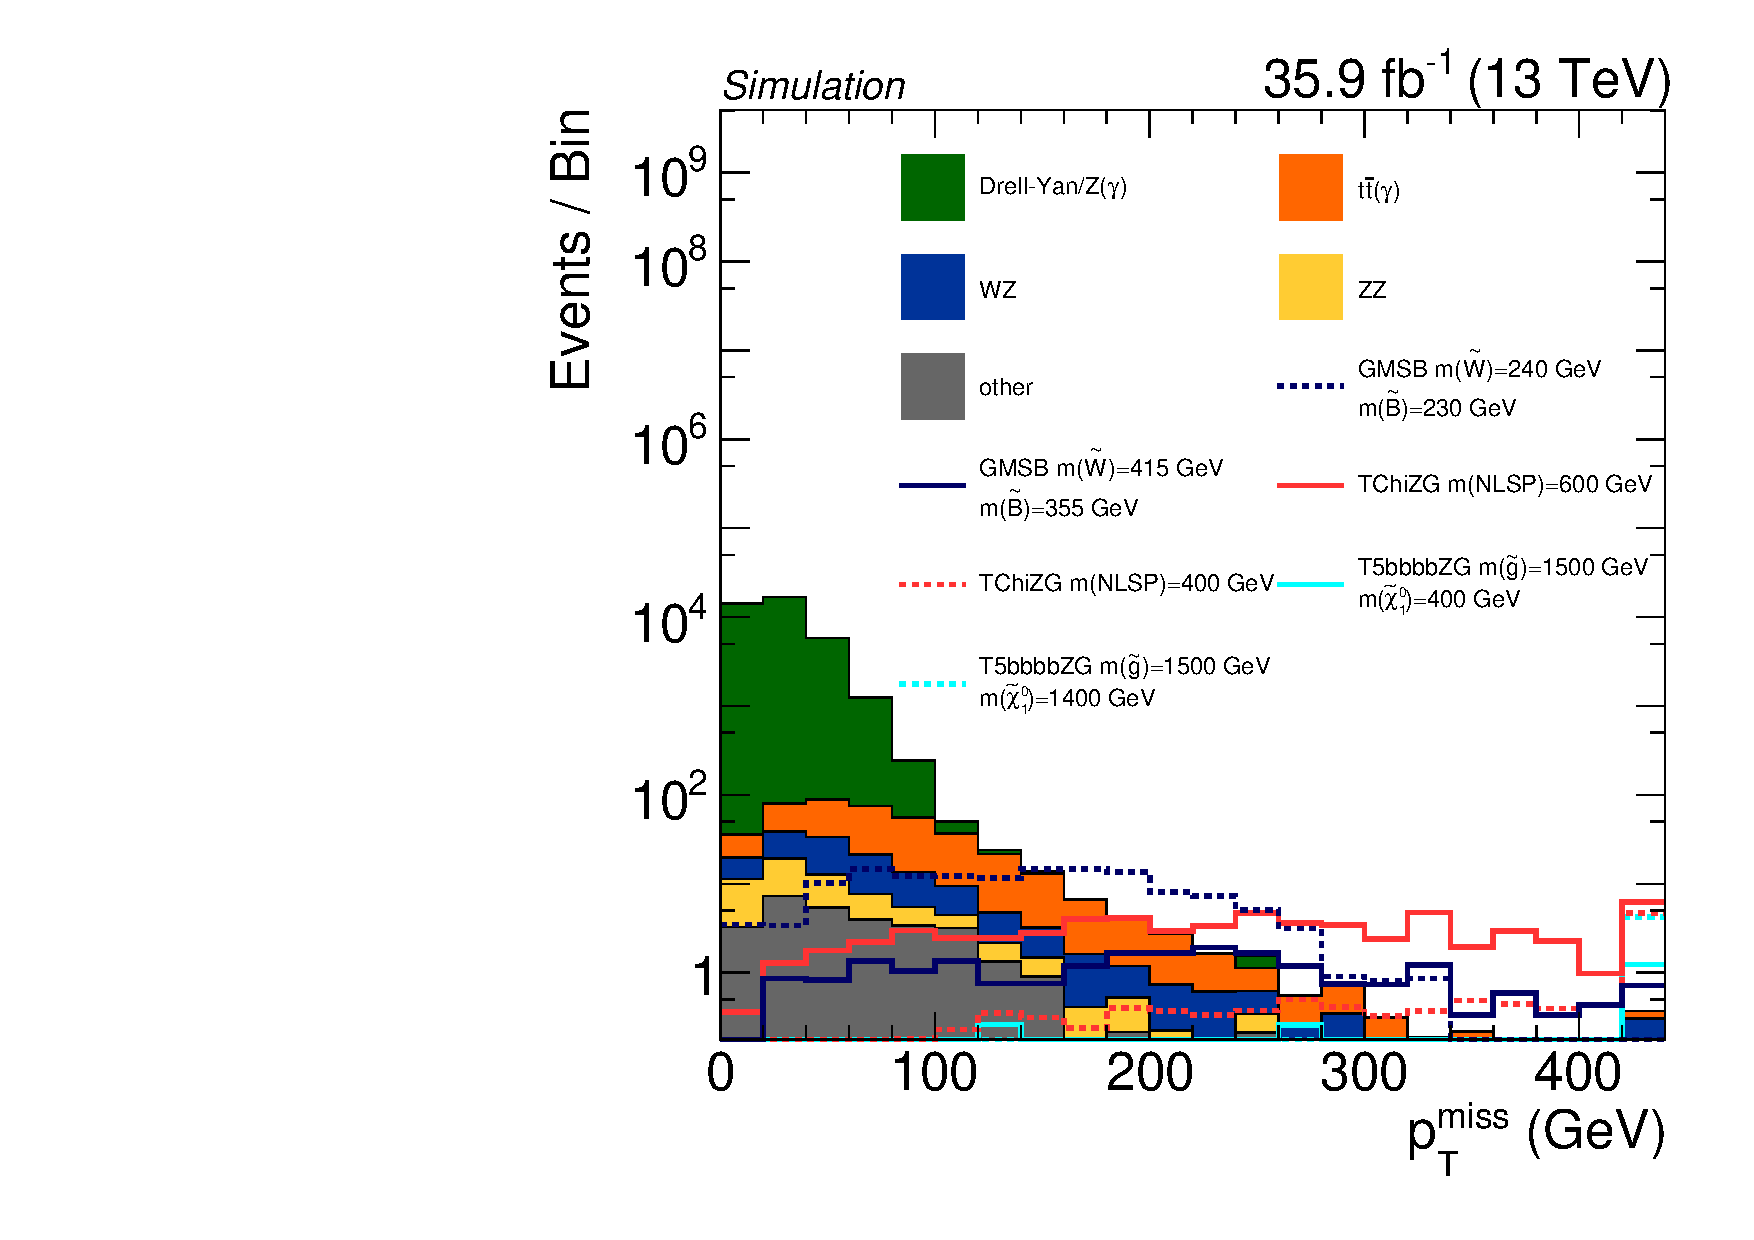
\includegraphics[width=\pairwidth]{figures/mt2/onZ_LL_met_log}
 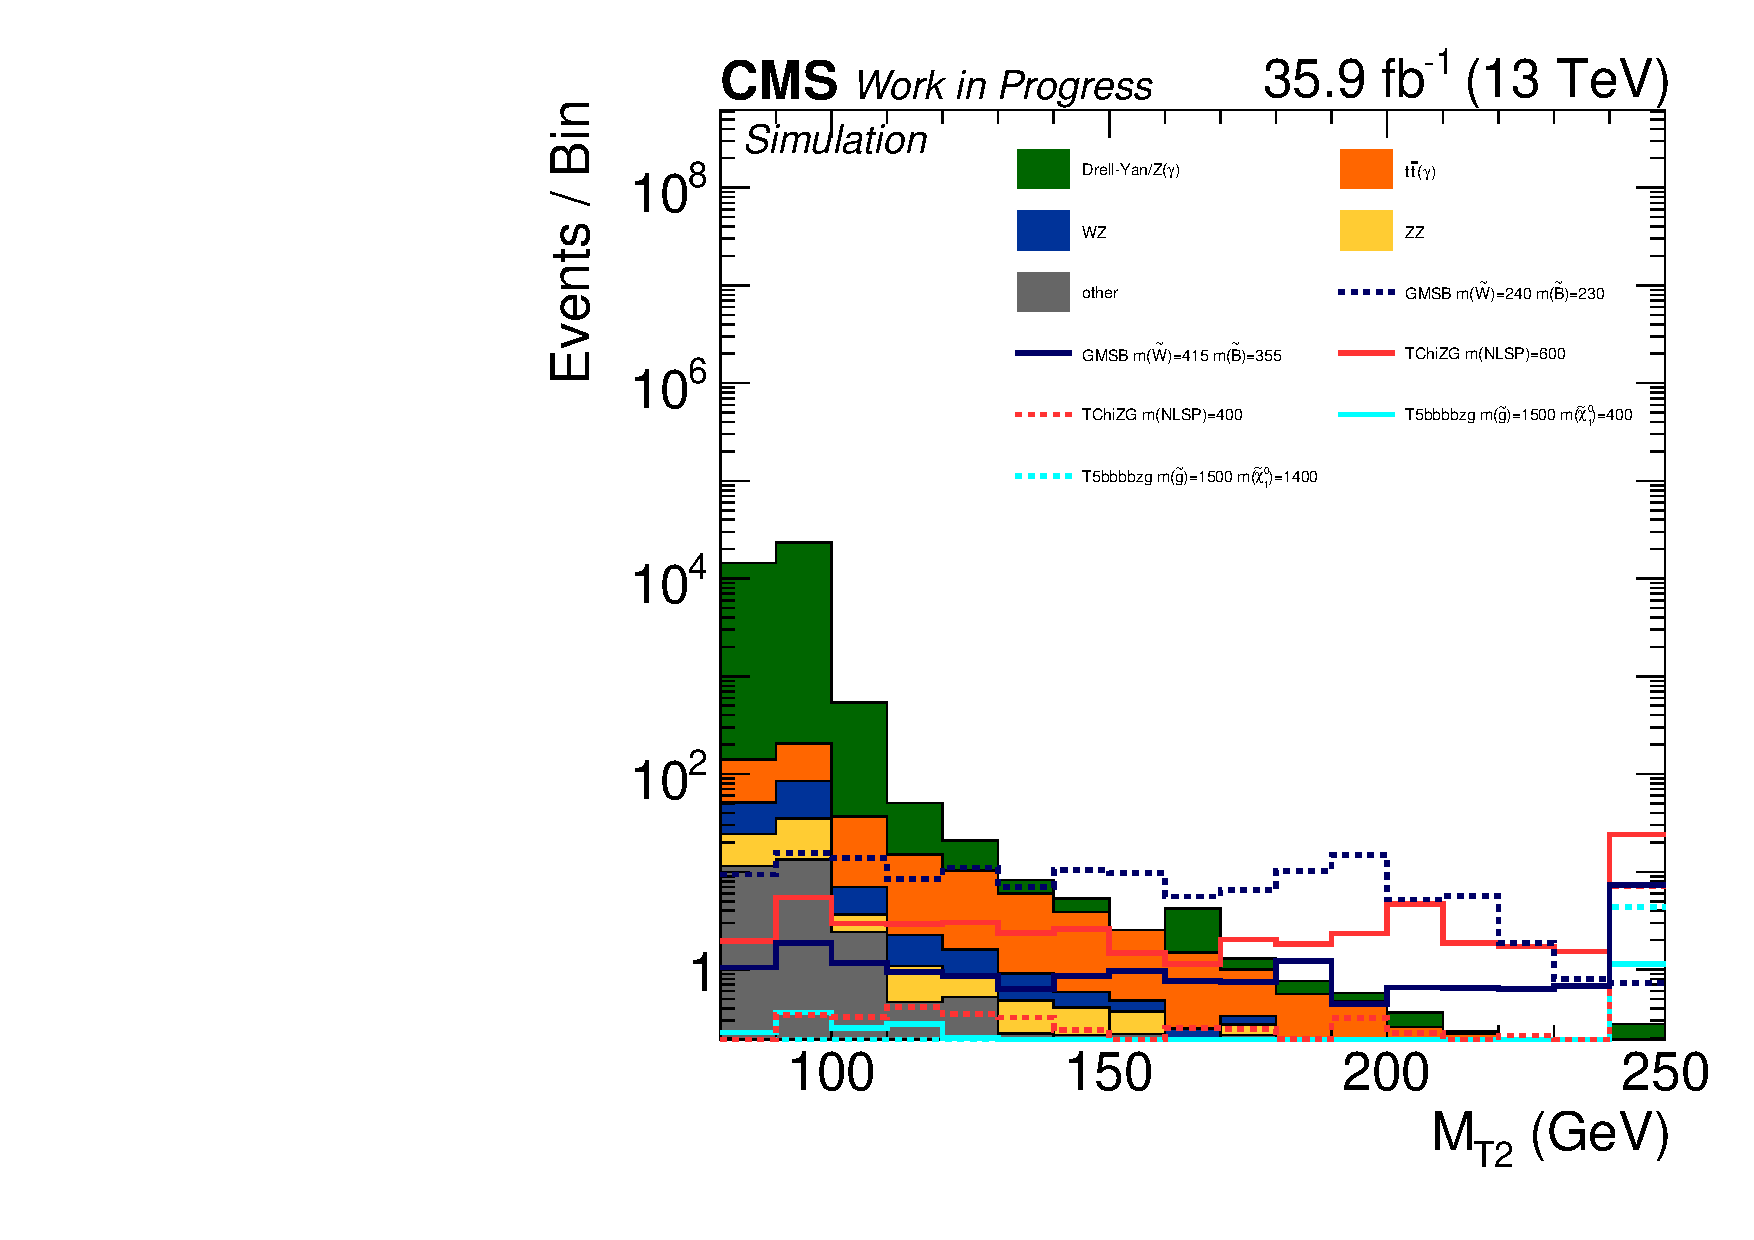
\includegraphics[width=\pairwidth]{figures/mt2/onZ_LL_mt2_log}
 \caption{Stacked background and different signal points against $\ptmiss$ (left) and the stransverse mass $\mtTwo$ (right). Both are obtained from simulation. For each signal model two different signal points are shown. For their mass paramaters refer to the legend in the plots.}
 \label{fig:SRvariables}
\end{figure}
Hence, the SR is defined by the following criteria:
\begin{itemize}
 \item $\ptmiss>150\GeV$,
 \item $\mtTwo>100\GeV$.
\end{itemize}
The final SR is binned in two search bins in the $\ptmiss$ distribution, one ranging from $150$ to $200\GeV$, and the second one ranging from $200\GeV$ to infinity, see \refSec{sec:results}.

\subsection{Control regions}\label{sec:CR}
Different control regions (CRs) are defined for the four main background contributions, in order develop a background prediction for the corresponding background. These CRs are built such, that they are fully orthogonal to the signal region and among each other and include a large amount of events for precise studies. The main groups of backgrounds are $\ttbar(\PGg)$, DY/$\PZ(\PGg)$, $\PW\PZ$, and $\PZ\PZ$ production.

\subsubsection*{$\ttbar(\PGg)$ - control region}
To obtain a CR for the $\ttbar(\PGg)$ background, the flavor symmetry of the process is exploited. The two top quarks can decay independently with the same probability to an electron or a muon, resulting in an equal number of same flavor and different flavor final state events. The different flavor triggers are needed to guarantee a basis data set containing a sufficient amount of events. In addition, the background can be studied in the same high $\ptmiss$ and $\mtTwo$ regions where the SR is defined due to the underlying symmetry of the dilepton production. The preselection criteria need to be adjusted accordingly, resulting in a CR definition of
\begin{itemize}
 \item exactly one different flavor - opposite charge (DFOC) lepton pair ($\Pe\Pgm$),
 \item at least one photon,
 \item $\Delta R(\ell_1,\PGg)>0.3$ and $\Delta R(\ell_2,\PGg)>0.3$.
\end{itemize}
The invariant dilepton mass window requirement is removed from he preselection, since the reconstructed dilepton mass is not in coincidence with the Z boson mass. In contrast, it shows a continuous distribution different from the top quark mass, because the neutrinos originating from the leptonic top decays cannot be reconstructed individually and are therefore not considered in the calculation. The requirement being responsible for the orthogonality to the SR is the different dilepton composition requirement.
\subsubsection*{Drell-Yan/$\PZ(\PGg)$ - control region}
The Drell-Yan/$\PZ(\PGg)$ background has nearly the same phenomenological topology as the SUSY signal, except for lower missing transverse momentum, since it is mainly present due to mismeasurements of jets. Therefore, the $\ptmiss$ distribution of the Drell-Yan/$\PZ(\PGg)$ background is defined by the $\ptmiss$ resolution of the detector and reconstruction. The final control region definition on top of the preselection reads
\begin{itemize}
 \item $\ptmiss<100\GeV$.
\end{itemize}
This region is orthogonal to the SR per definition due to the inverted $\ptmiss$ requirement.
\subsubsection*{$\PW\PZ$ - control region}
In order to obtain a high purity $\PW\PZ$ control region, the SFOC dilepton criteria is adjusted such, that the fully leptonic decay of the diboson system is studied. As in the preselection, a SFOC lepton pair is required, but the additional lepton veto is removed. Hence, the existence of third lepton, which can be either an electron or a muon, is demanded. This ensures exclusivity between the SR and this CR. Since the $\PW\to2\ell\PGn$ boson decays are selected, with the help of additional $\ptmiss$ and $m_{T}$ requirements a further purification of $\PW\PZ$ diboson production events is achieved. the transverse mass $m_{T}$ is calculated using the third lepton assumed to come from the $\PW$ boson and the missing transverse momentum, and is therefore an estimate for the $\PW$ boson mass. In the identification of the lepton pair belonging to the decayed $\PZ$ boson, all combinations fulfilling flavor and charge requirements are tested. In case of multiple valid combinations, the combination with the invariant dilepton mass closest to the Z boson mass is chosen. To ensure a selection with a suitable amount of data, since the cross section for diboson production is rather low, the existence of at least one photon from the preselection is removed. The final region selection reads
\begin{itemize}
 \item exactly one SFOC lepton pair ($\Pe\Pe$ or $\PGm\PGm$),
 \item exactly one additional third lepton ($\Pe$ or $\Pgm$),
 \item $\Delta R(\ell_1,\PGg)>0.3$ and $\Delta R(\ell_2,\PGg)>0.3$,
 \item $81\GeV<m_{\ell\ell}<101\GeV$,
 \item $\ptmiss>70\GeV$,
 \item $m_{T}(\ptvecmiss,\mathrm{p_{\ell_3}})>50\GeV$.
\end{itemize}
\subsubsection*{$\PZ\PZ$ - control region}\label{sec:VR}
The strategy to achieve a pure $\PZ\PZ$ diboson selection that is not overlapping with the SR selection is very similar to the $\PW\PZ$ CR selection described above. By selecting events, where both $\PZ$ bosons decay leptonically to charged leptons ($\Pe\Pe$ or $\PGm\PGm$), per definition an exclusive control region is obtained. As in the $\PW\PZ$ CR selection, flavor and charge requirements are considered to construct $\Z$ boson candidates from the four selected leptons. In cases, where multiple valid solutions for the reconstruction of two $\PZ$ bosons exist, the possibility with the first Z boson candidate mass closest to the nominal Z boson mass is chosen. The second Z boson candidate has to fulfill a looser mass agreement compared to the first one. Also, the existence of a photon in the event is not required. In total the selection criteria read:
\begin{itemize}
 \item exactly two SFOC lepton pairs ($\Pe\Pe$ or $\PGm\PGm$),
 \item $\Delta R(\ell_1,\PGg)>0.3$ and $\Delta R(\ell_2,\PGg)>0.3$ for the first pair,
 \item $76\GeV<m_{\ell\ell}<106\GeV$ for the mass of the first Z boson candidate,
 \item $50\GeV<m_{\ell\ell}<130\GeV$ for the mass of the second Z boson candidate.
\end{itemize}
\subsubsection{Validation region}
An additional validation region (VR) is constructed, where the developed background predictions are verified by performing data to background prediction comparisons. Therefore, it is convenient to choose the VR close in phase space to the SR. This is achieved by applying the same selection requirements as for the SR, but demanding either the $\ptmiss$ the $\mtTwo$ requirement to fail. Hence, the VR is built as a sideband to the SR. The VR must also not overlap with the DY/$\PZ(\PGg)$ CR, thus a minimal $\ptmiss$ requirement needs to be imposed. The selection requirements for the VR in addition to the preselection are the following:
\begin{itemize}
 \item $\ptmiss>100\GeV$,
 \item either $\ptmiss<150\GeV$ or $\mtTwo>100\GeV$.
\end{itemize}
\\
A visualization of the signal, validation, and DY/$\PZ(\PGg)$ control region definitions in the $\mtTwo$-$\ptmiss$ plane can be found in \refFig{fig:Regions}. Two dimensional histograms for the number of expected events motivating the region definitions are shown in \refFig{fig:Regions2} for all background processes, together with distributions of different benchmark points for all three considered signal models.
\begin{figure}[tbp]
 \centering
 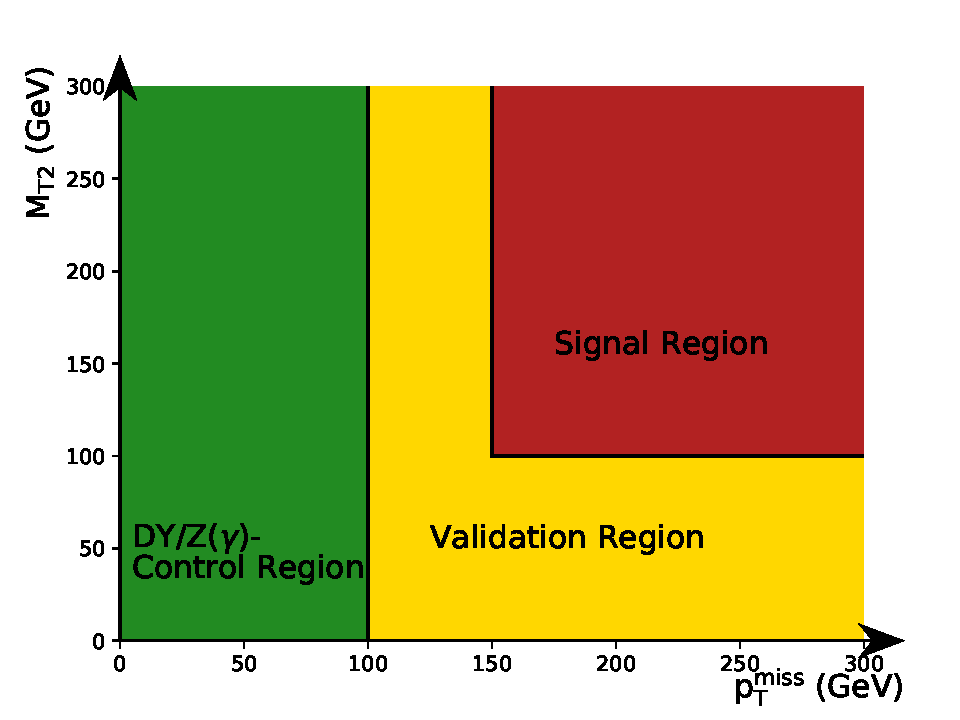
\includegraphics[width=\pairwidth]{figures/figures/regions}
 \caption{Visualization of the definition of the signal, validation and DY/$\PZ(\PGg)$ control region in the $\mtTwo$-$\ptmiss$ plane.}
 \label{fig:Regions}
\end{figure}
These distributions show also specific features of the considered signal models regarding important kinematic observables. Because the \texttt{TChiZG} model is a one parameter scan, and the only free parameter is the NLSP mass, it directly determines the maximum amount of transverse momentum for the decay products and thus directly the boson $\pt$ and the $\ptmiss$ originating from the gravitinos. Hence, $\ptmiss$ and $\mtTwo$ calculated from the bosons and $\ptmiss$ are strongly correlated. Also, the endpoints of the $\ptmiss$ and $\mtTwo$ distributions are of the same order and coincide with the NLSP mass. In case of the strong SMS, this is not directly the case. Since this is a two dimensional parameter scan, the event kinematic depends also on the mass difference of the gluino and the NLSP mass, as discussed in \refSec{sec:SMS}. In cases where the mass difference is small, the kinematics evolve similar as for the EWK SMS, while for larger mass differences, as shown in \refFig{fig:Regions2}, the correlation between $\mtTwo$ and $\ptmiss$ is much weaker and the distributions are much broader. The distributions of the GMSB model behave like a mixture of the two SMSs, depending on the wino and bino masses.\\
And most importantly, the signal events mainly populate the SR for all models, with small contributions in the CRs and the VR, while the majority of the background events contribute to the DY/$\PZ(\PGg)$ CR and a minor part to the VR. Only a minority contributes to the SR, as it is desired. In total, a good separation between background and signal is achieved.

\begin{figure}[tbp]
 \centering
 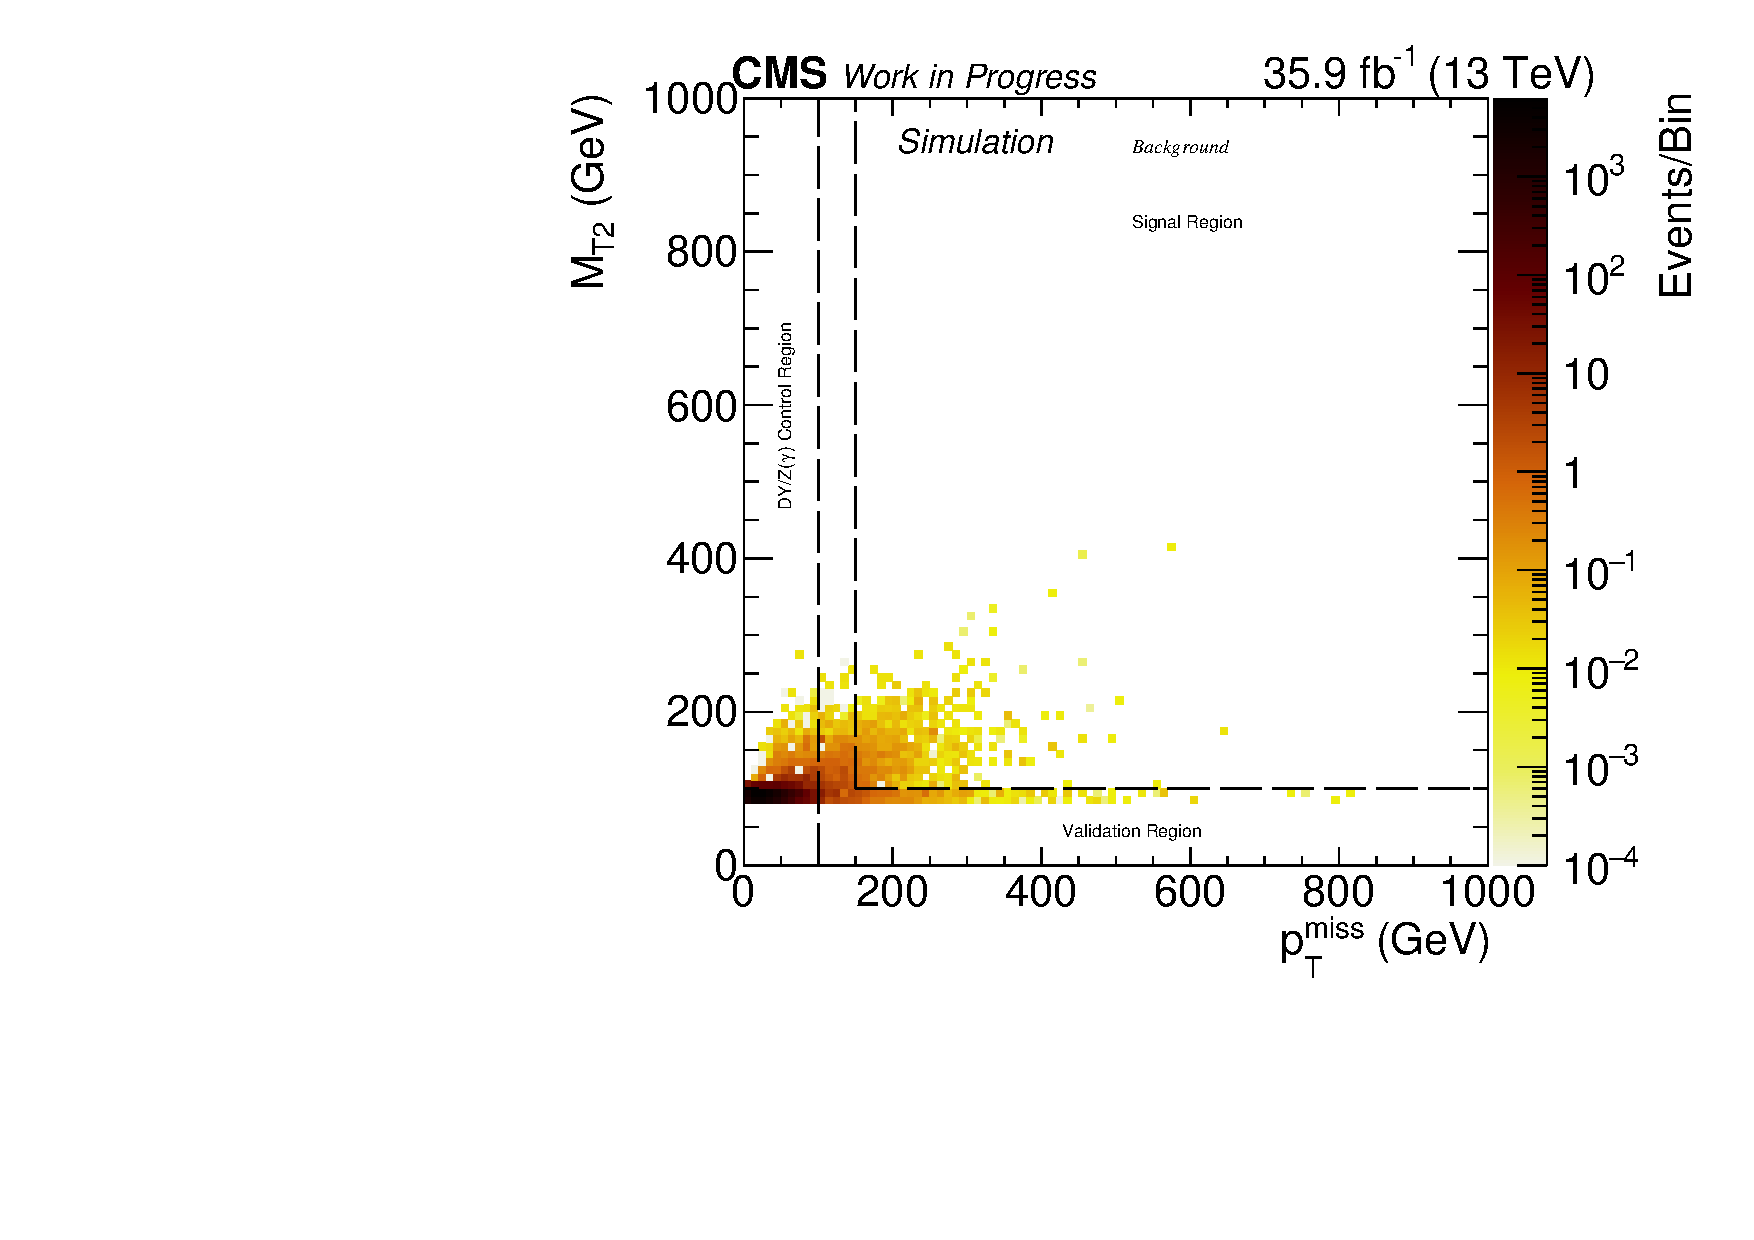
\includegraphics[width=\pairwidth]{figures/plots_2d/DataMC_sameHistograms_LL+signal_onZ__LL__MetMt2_bkg_}
 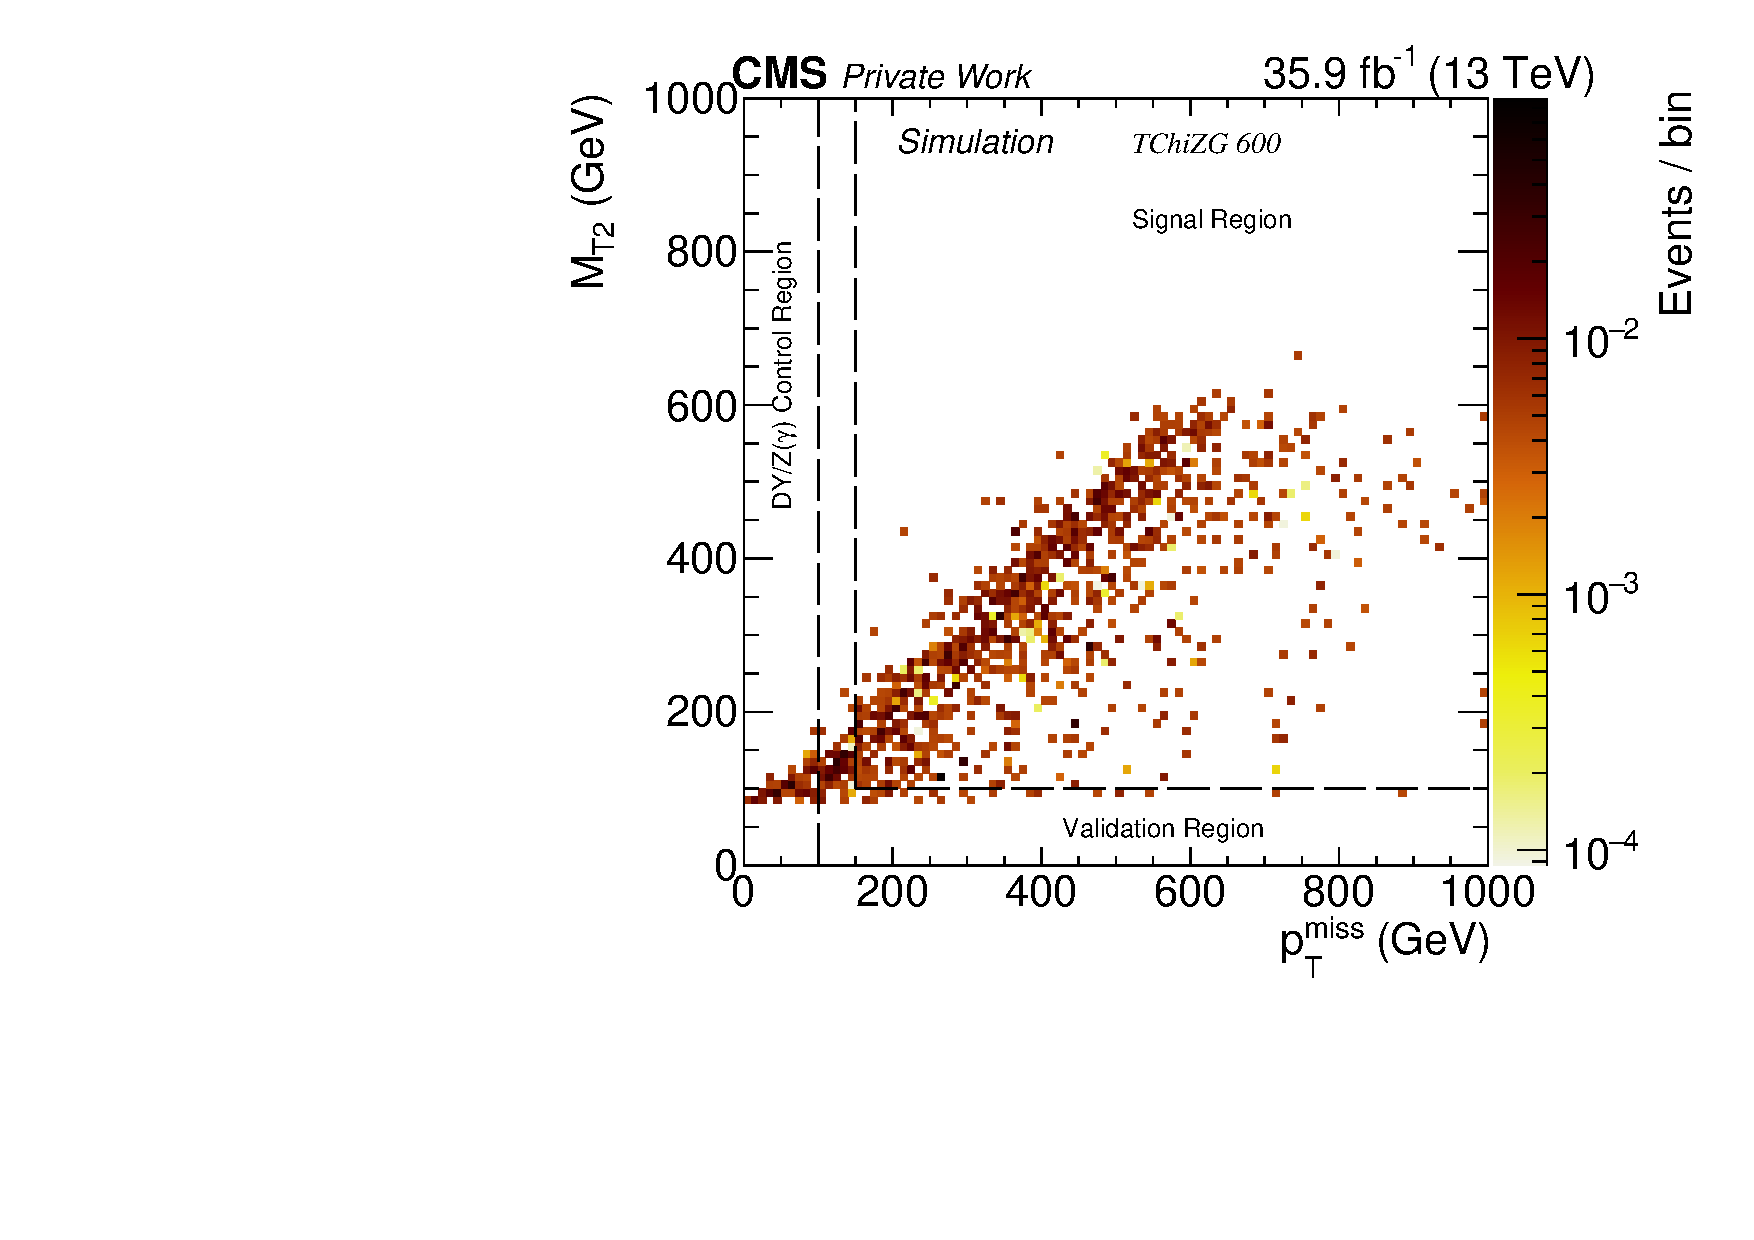
\includegraphics[width=\pairwidth]{figures/plots_2d/DataMC_sameHistograms_LL+signal_onZ__LL__MetMt2_SIG_tching600_}\\
 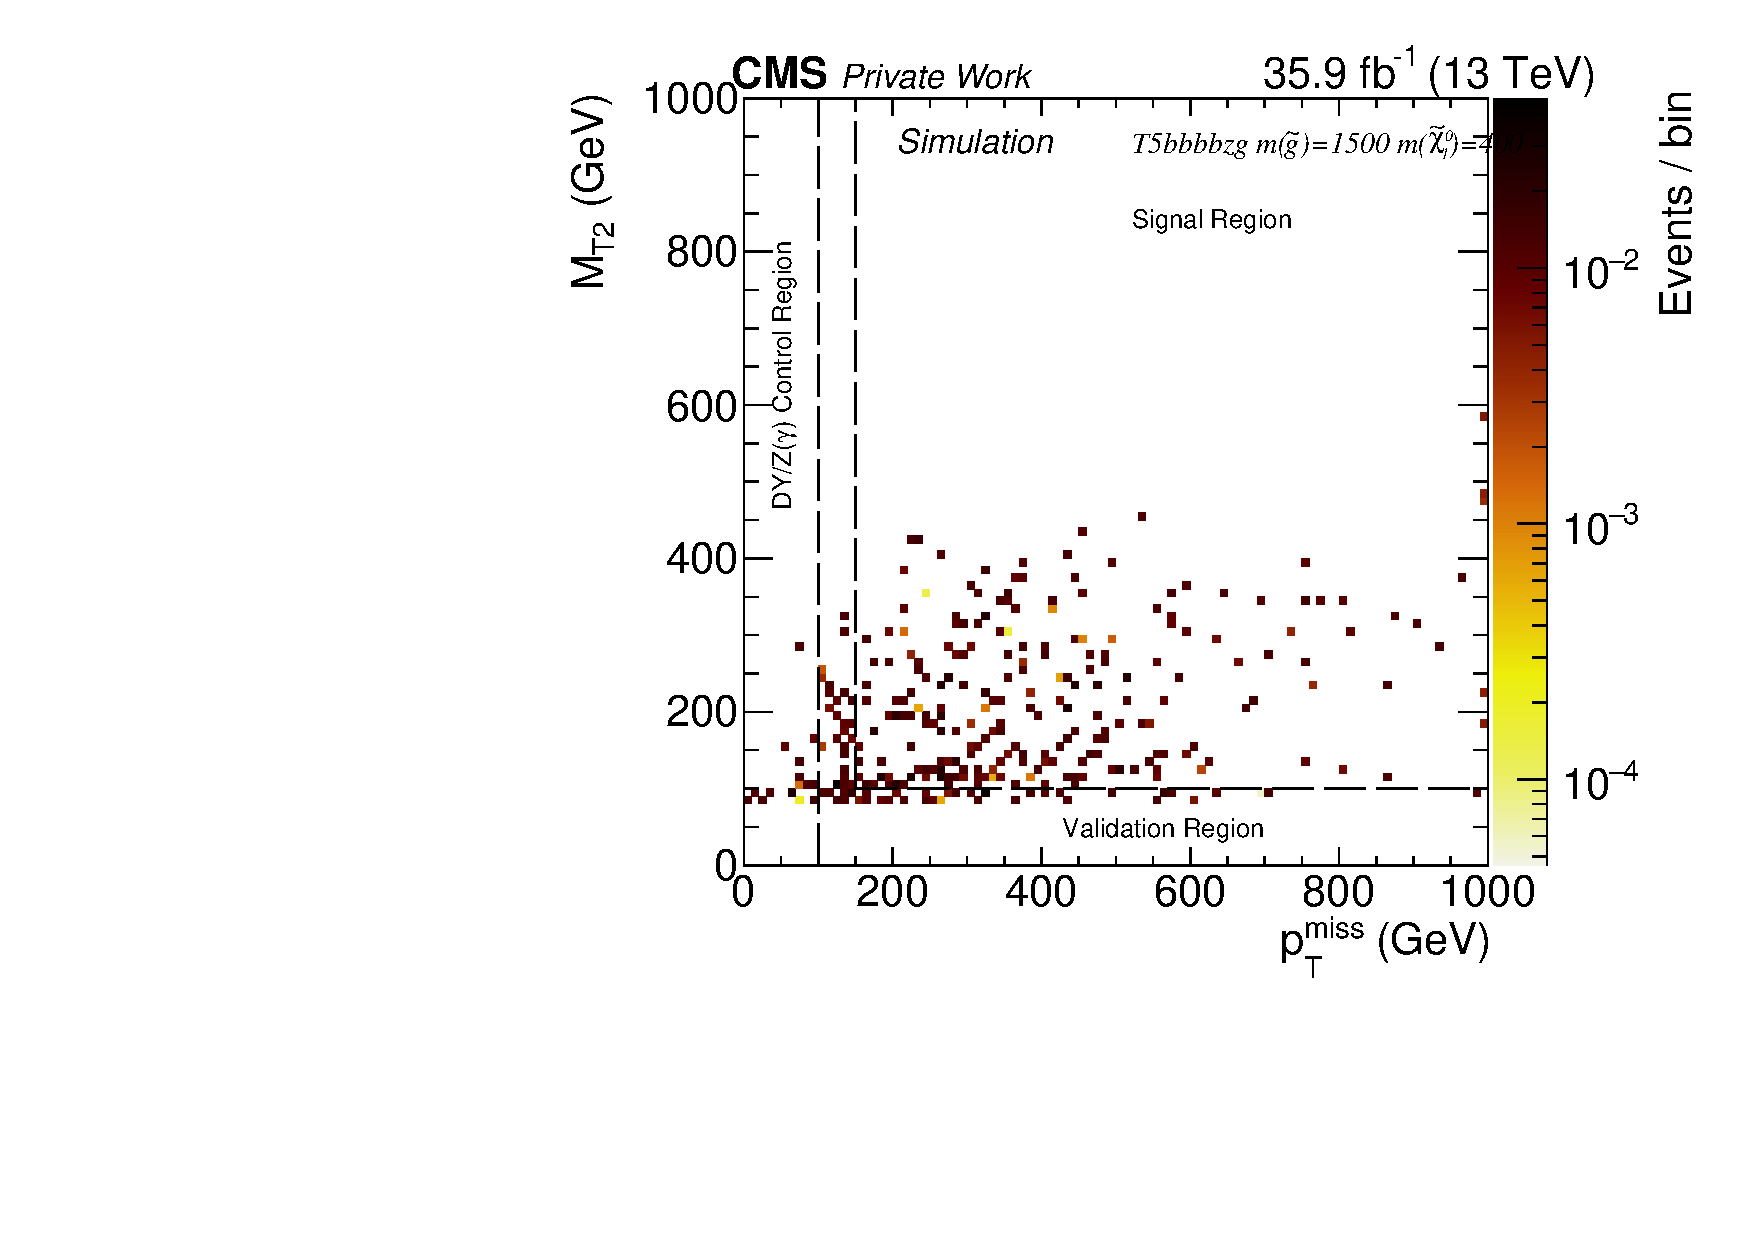
\includegraphics[width=\pairwidth]{figures/plots_2d/DataMC_sameHistograms_LL+signal_onZ__LL__MetMt2_SIG_t5bbbbzg_1500_400_}
 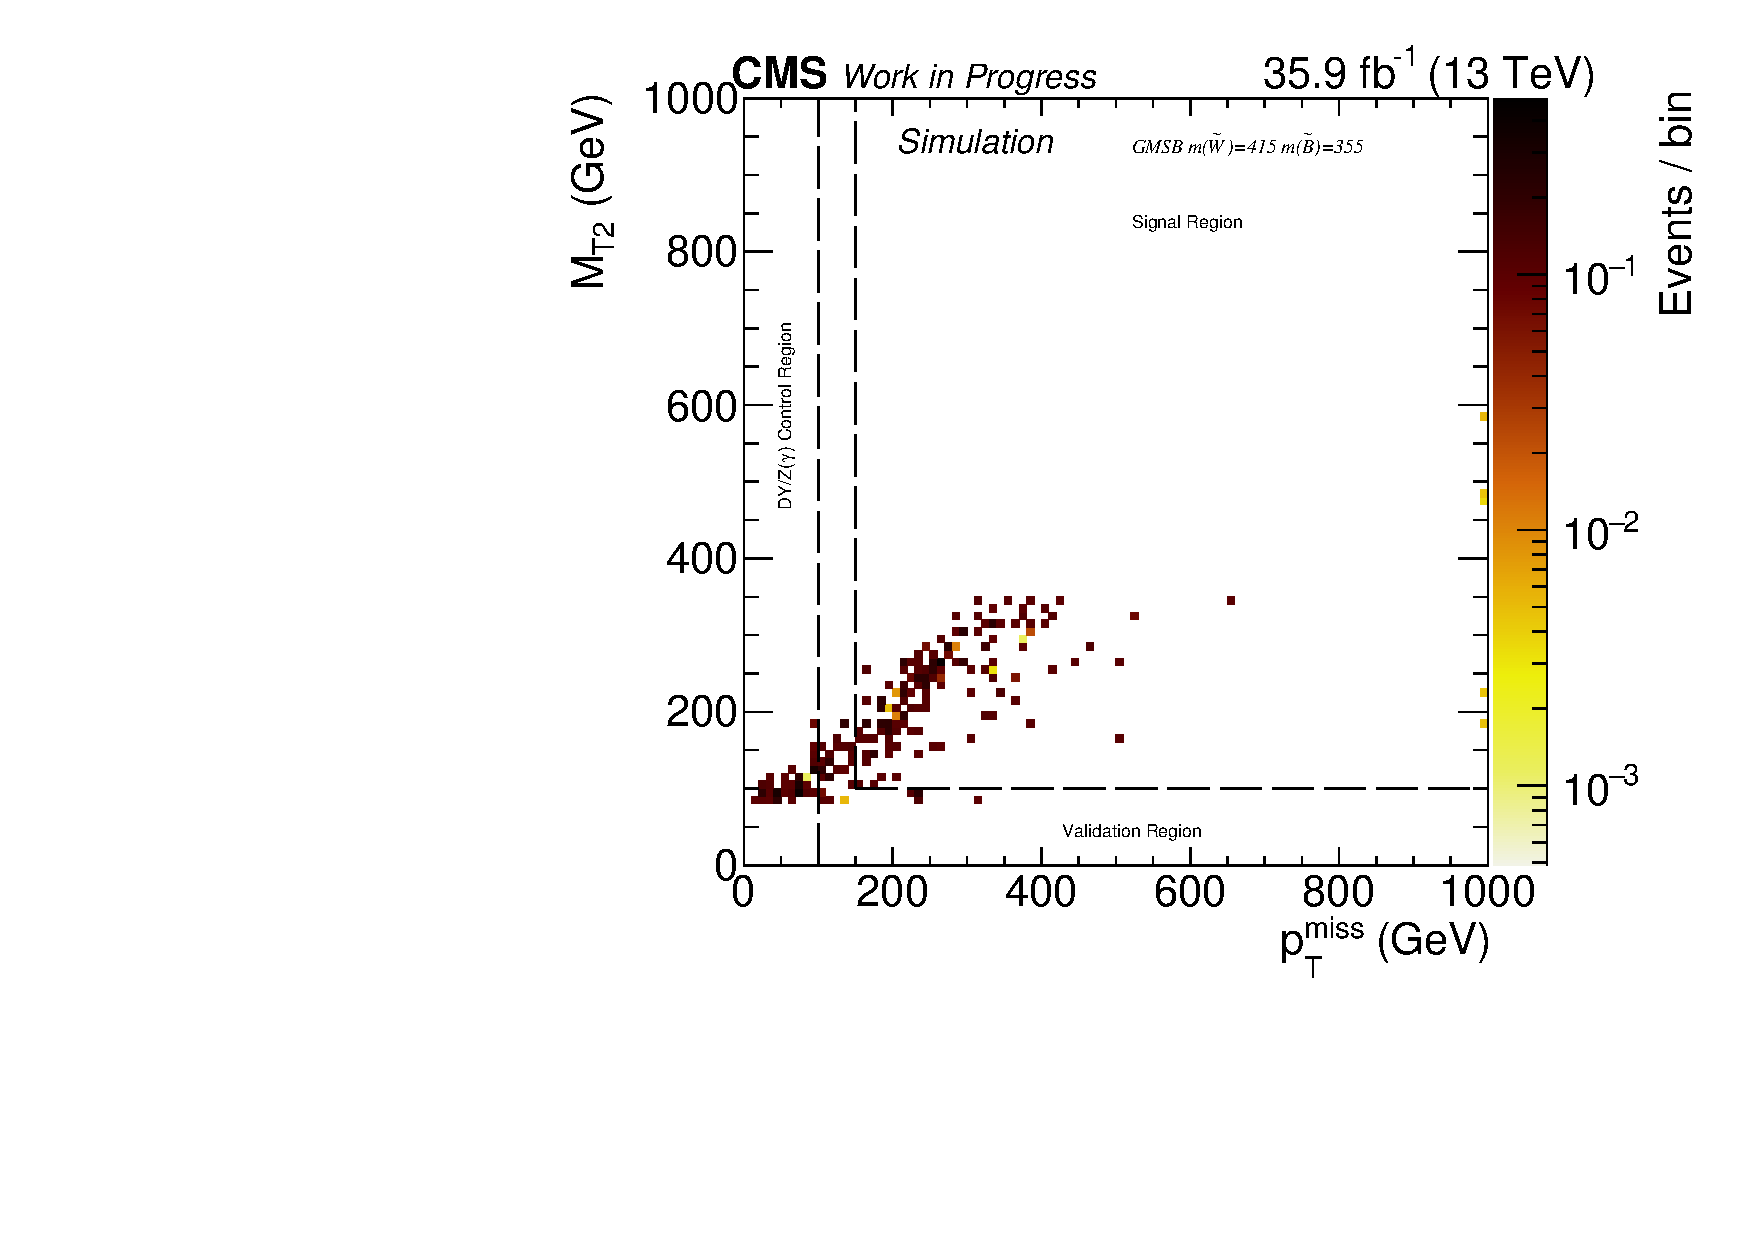
\includegraphics[width=\pairwidth]{figures/plots_2d/DataMC_sameHistograms_LL+signal_onZ__LL__MetMt2_SIG_gmsb_415_355_}
 \caption{Distribution of the total number of expected background events in the $\mtTwo$-$\ptmiss$ plane (upper left). Distributions for the number of expected signal events for the \texttt{TChiZG} SMS with an NLSP mass of $600\GeV$ (upper right), the \texttt{T5bbbbZG} SMS with a gluino mass of $1.5\TeV$ and a neutralino mass of $400\GeV$ (bottom left), and the GMSB model with $m(\widetilde{W}=455\GeV)$ and $m(\widetilde{B}=355\GeV)$ (bottom right).}
 \label{fig:Regions2}
\end{figure}



\section{Background estimation}\label{sec:BKG}
In this section the used background estimation methods are discussed, including the study of systematic effects. The total background is composited of $\ttbar(\PGg)$ production, Drell-Yan and $\PZ(\PGg)$ events, $\PW\PZ$ and $\PZ\PZ$ diboson production, and a remaining group of backgrounds, composited of \eg singletop and triboson production (See \refSec{sec:Simulation} and \refSec{sec:CR}). The relative amounts for all background contributions in the two SR bins are depicted in \refFig{fig:PieCharts}. The most dominating background is $\ttbar(\PGg)$, followed by $\PW\PZ$, $\PZ\PZ$, and Drell-Yan/$\PZ(\PGg)$.\\
The leptonic decays of the top pairs generated in association with a photon significantly contribute to the SR, because the final state signatures appear very similar to those of the SUSY models and the production cross section is very high. If both $\PW$ bosons decay leptonically, a SFOC lepton pair in connection with neutrinos can be produced, that generate a large amount of $\ptmiss$ in the detector. Also real photons can be produced in the hard interaction, or can be radiated off in the initial or the final state by participating charged particles. Since the total mass of the top pair cannot be reconstructed due to the momentum imbalance, there is a sufficient probability to measure an invariant dilepton mass close to the Z boson mass.\\
In the Drell-Yan process, in context with FSR or ISR, and in $\PZ\PGg$ production, directly an on-shell Z boson is produced, thus the $\m_{\ell\ell}$ requirement for the dileptons in the SR is fulfilled. Although additional a photon is produced, this background does not contribute significantly to the SR, because only nongenuine $\ptmiss$ is generated in the process due to mismeasurements and therefore the $\ptmiss$ distribution drops steeply.\\
$\PW\PZ$ production is also an important background for this search, since the $\PW$ boson can decay leptonically and therefore creates a sufficient amount of genuine $\ptmiss$ to pass the SR requirements. While a photon can be generated in all possible radiation processes, an additional electron or jet originating from the $\PW$ boson can fake a photon signature in the detector. In cases of real photons, the additional lepton can also be lost in the reconstruction.\\
Lastly, the $\PZ\PZ$ event signature can be very similar to the one expected from the considered SUSY signals. One boson can decay to a pair of charged leptons, while the other decays to neutrinos leading to a large amount of $\ptmiss$ in the event. Together with FSR or ISR of a photon, it mimics the signal topology in many ways.\\
If the different background processes are compared, the diboson processes may have a more similar event kinematic than the $\ttbar(\PGg)$ process, but due to the lower diboson production cross sections, and the small branching fraction for a $\PZ$ or $\PW$ boson to decay to charged leptons, the $\ttbar(\PGg)$ background dominates the other contributions.\\
\begin{figure}[tbp]
 \centering
 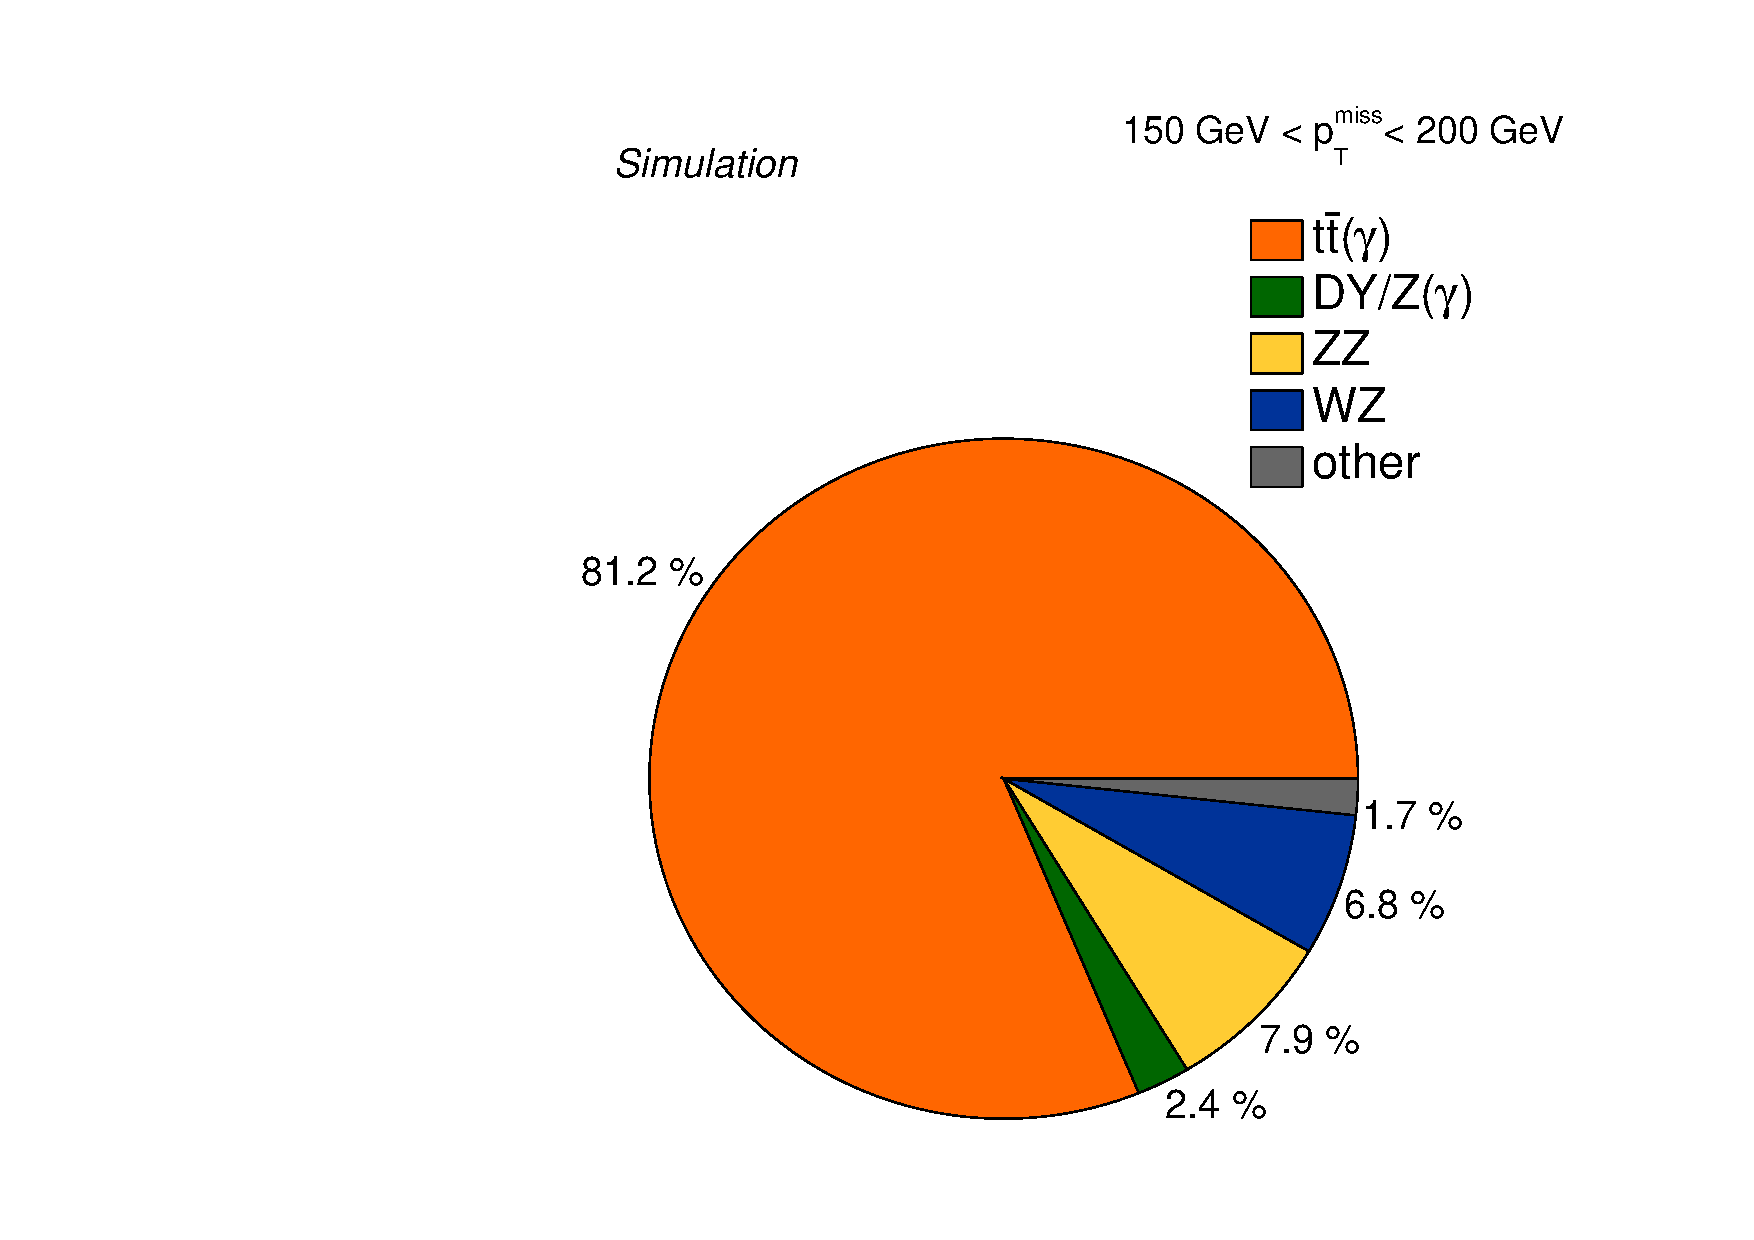
\includegraphics[width=\pairwidth]{figures/figures/pie1}
 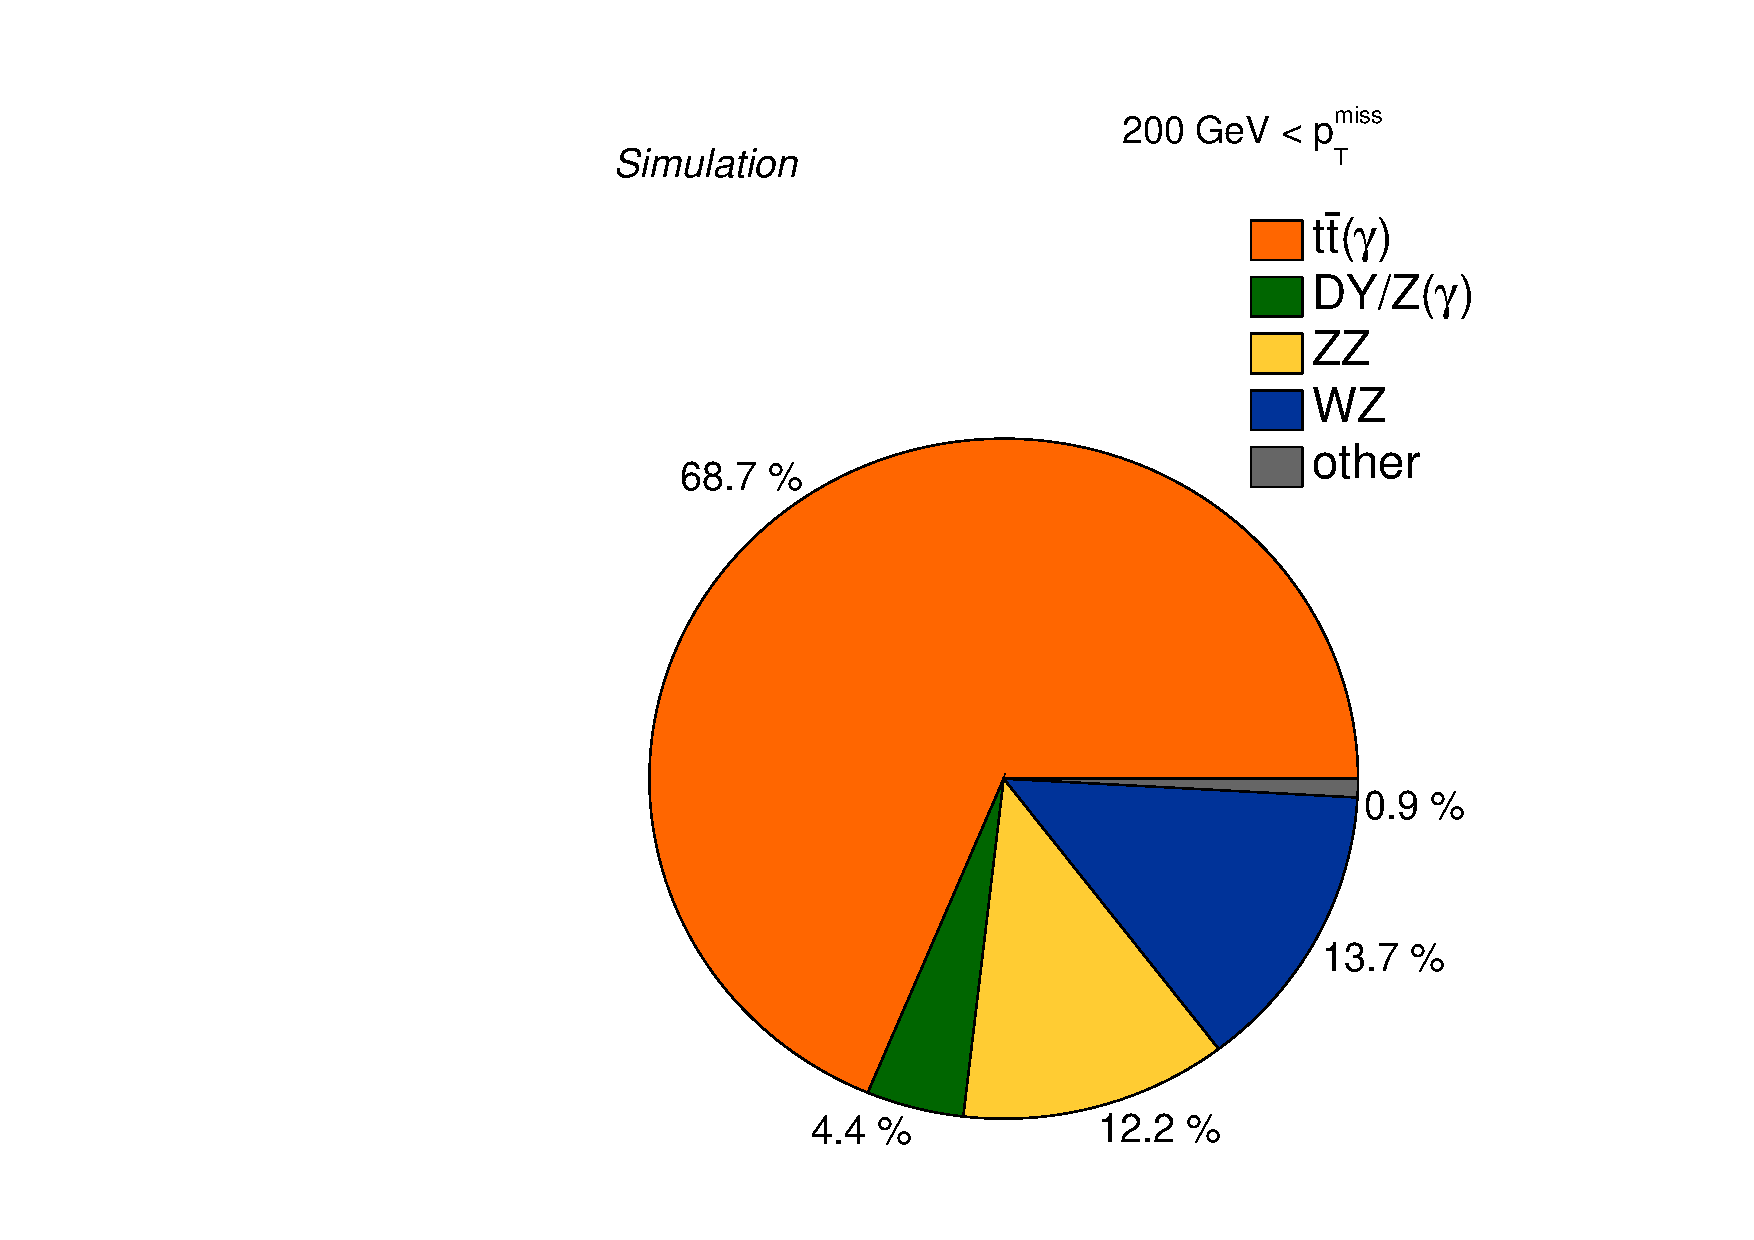
\includegraphics[width=\pairwidth]{figures/figures/pie2}
 \caption{Relative amounts for all group of considered backgrounds for the two search bins in the SR.}
 \label{fig:PieCharts}
\end{figure}
The strategy to perform a sophisticated background prediction is based on MC simulation for all backgrounds. As mentioned in \refSec{sec:CR}, different CRs are developed, that are enriched with corresponding background events. In those CRs, scale factors (SF) $\alpha_i$ are calculated by scaling the total simulation to the measured data yield. Contributions of other backgrounds in the CR are considered in the calculation by fixing their contribution, thus only one background is scaled. The SFs are calculated via the following formula:
\begin{align}
 1                        & = \frac{\#Data}{\#FixedBackground+\alpha_i\cdot\#BackgroundToScale} \\
 \Longrightarrow \alpha_i & = \frac{\#Data-\#FixedBackground}{\#BackgroundToScale}.             
\end{align}
Due to the used method, which is performed similar in each CR, possible uncertainties in the normalization cancel, and only uncertainties in the shape need to be considered, see~\refSec{sec:Syst}. The uncertainty arising from the SF calculation is purely of statistical origin, and is calculated via error propagation
\begin{equation}
 \sigma_{\alpha_i}^2 = \sigma_{D}^2 \cdot \left(\frac{D}{B}\right)^2 + \sigma_{F}^2 \cdot \left(\frac{F}{B}\right)^2 + \sigma_{B}^2 \cdot \left(\frac{D-F}{B^2}\right)^2,
\end{equation}
where $B=\#BackgroundToScale$, $F=\#FixedBackground$, $D=\#Data$, and $\sigma_i$ are the corresponding statistical uncertainties. These are assumed to be uncorrelated Poissonian uncertainties, and can be calculated via $\sigma_i=\sqrt{N_i}$, where $N$ is the associated total integral in the selection. In the case of MC simulation, for the calculation of the SF the normalized event yield is used, whereas in the error calculation the pure MC event count is considered to reflect the underlying precision of the simulation. These method is referred to as the "integral method" in the following.\\
In each CR, all other backgrounds have of course an influence, since their contributions are not negligible. Therefore, the order of SF determination can introduce a bias. To minimize this effect, the SFs are calculated in descending order of the purity of the background sample. At first, the $\PZ\PZ$ SF is determined, followed by DY/$\PZ(\PGg)$, $\ttbar(\PGg)$, and $\PW\PZ$. However, the background estimations are discussed in a different order, starting with the most important background, $\ttbar(\PGg)$. The systematic uncertainty arising from the choice of order is discussed in \refSec{sec:Syst}.\\
After determining all SFs, the background prediction will be tested in the VR. Therefore, the simulated backgrounds in the VR will be scaled accordingly, and the result will be investigated, see \refSec{sec:Validation}.



\subsection{Top pair production in association with a photon}\label{sec:ttbar}
As shown in \refFig{fig:PieCharts}, the main background contribution is $\ttbar(\PGg)$, which is composited of standard top pair production with and without photon radiation, and top-pair production in association with a photon, while the latter dominates. Both compositions will be determined together by rescaling the simulation, such that the integral of events of the MC simulation in the CR matches the integral of events in data as explained in \refSec{sec:BKG}. The raw and rescaled yields of the simulation, together with the observation in the CR are quoted in \refTab{tab:CRTT}. The overall purity of the selection is of the order of $84.62\%$. For the scaled event yields, only weights to account for the trigger efficiency correction and a global weight as mentioned in \refSec{sec:Simulation} to normalize the simulation to the physical expectation are made use of.
\begin{table}[tbp]
 \centering
 \caption{Yields in the $\ttbar(\PGg)$ CR for the pure simulation and measured data.}
 \label{tab:CRTT}
 \begin{tabular}{llll}
  
  process      & raw simulation & simulation & data                  \\\hline
  $\ttbar$     & 12077          & 416.93     &                       \\
  $\ttbar\PGg$ & 128396         & 1420.19    &                       \\\hline\hline
  sum          & 140473         & 1837.12    & \multirow{2}{*}{1750} \\
  other        & 14631          & 275.25     &                       
 \end{tabular}
\end{table}
With the integral method applied, the SF given in \refEq{eq:AlphaTT} is obtained.
\begin{equation}\label{eq:AlphaTT}
 \alpha_{\ttbar(\PGg)}=0.803 \pm 0.327 (stat.) [\hat{=}4.07\%].
\end{equation}
After application of $\alpha_{\ttbar(\PGg)}$, the number of events in data and total simulation match per definition.\\
Since the analyzed final state in this CR is very sensitive to higher order effects such as jet and photon radiation, and complex matrix elements are needed to describe the hard interaction, and these are very hard to model in the simulation, a SF differing from unity is not unexpected. Because the generation of MC simulation in general is time and resource consuming, simplifications are made on \eg radiation effects, and not all aspects of a specific process are calculated and generated at NLO, although \MCATNLO was used for the generation of the $\ttbar\PGg$ sample. NNLO electroweak effects can cause negative corrections for example due to destructive terms in higher order corrections. The uncertainty of the order of $4\%$ indicates, that a sufficient amount of events is present in the corresponding CR.\\
The resulting prediction shows a good agreement with data, as can be seen from the $\ptmiss$ and $\mtTwo$ distributions in the CR after rescaling in \refFig{fig:CRTT}. The uncertainty of the fit method is of statistical origin, and is treated as a systematic in the following. The agreement of additional important observables, such as the transverse momentum of the photon and both leptons, is also investigated, and no systematic deviation was found. To strengthen the confidence in the outcome, Kolmogorov-Smirnov~\cite{KS} tests are performed to study the shape agreement, which are based on the largest deviation between the two compared distributions. No significant shape disagreement is found, and the KS-values from the tests results are quoted on the plots for each individual distribution. KS-values $\ll1$ indicate disagreement between the input distributions, otherwise the distributions are considered to match.
\begin{figure}[tbp]
 \centering
 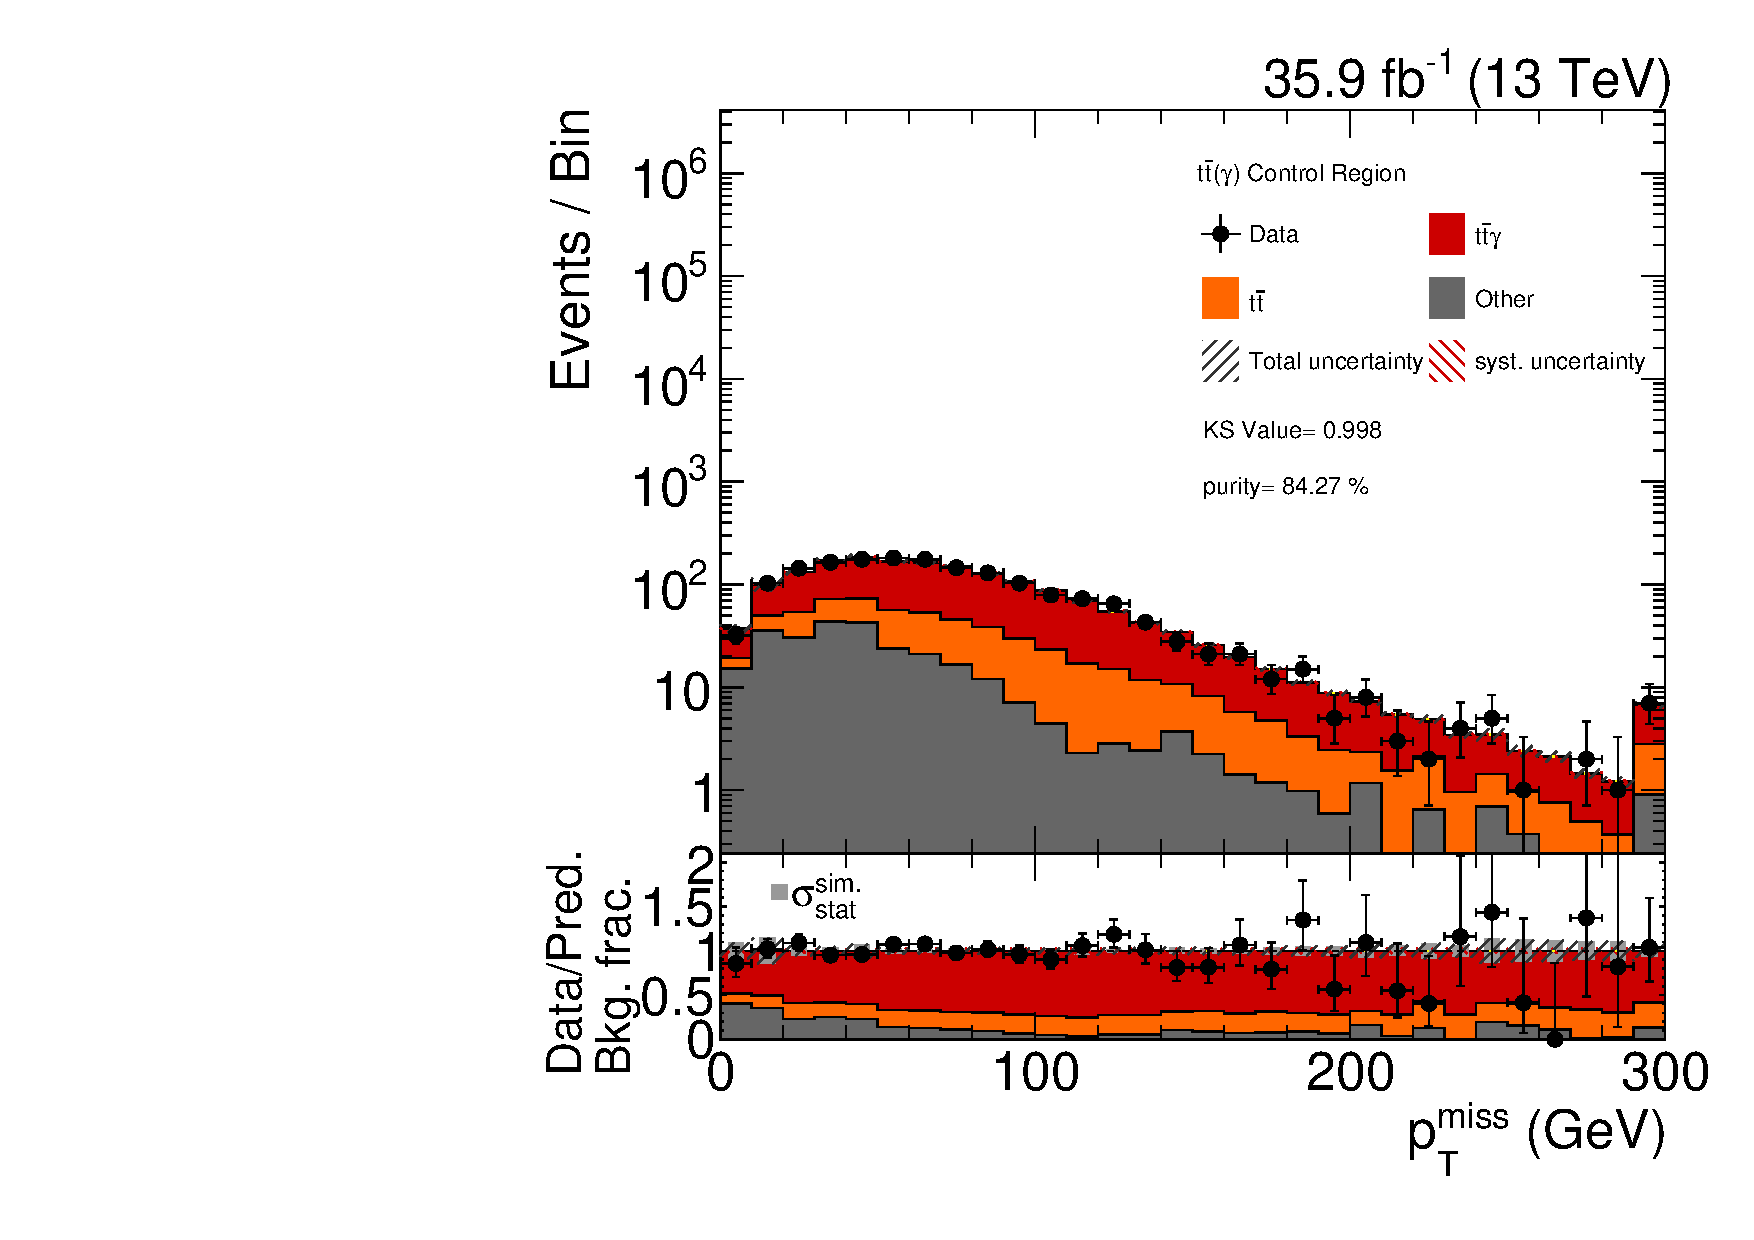
\includegraphics[width=\pairwidth]{figures/plots_CR_tt/CRTT_EM_nom_met_log}
 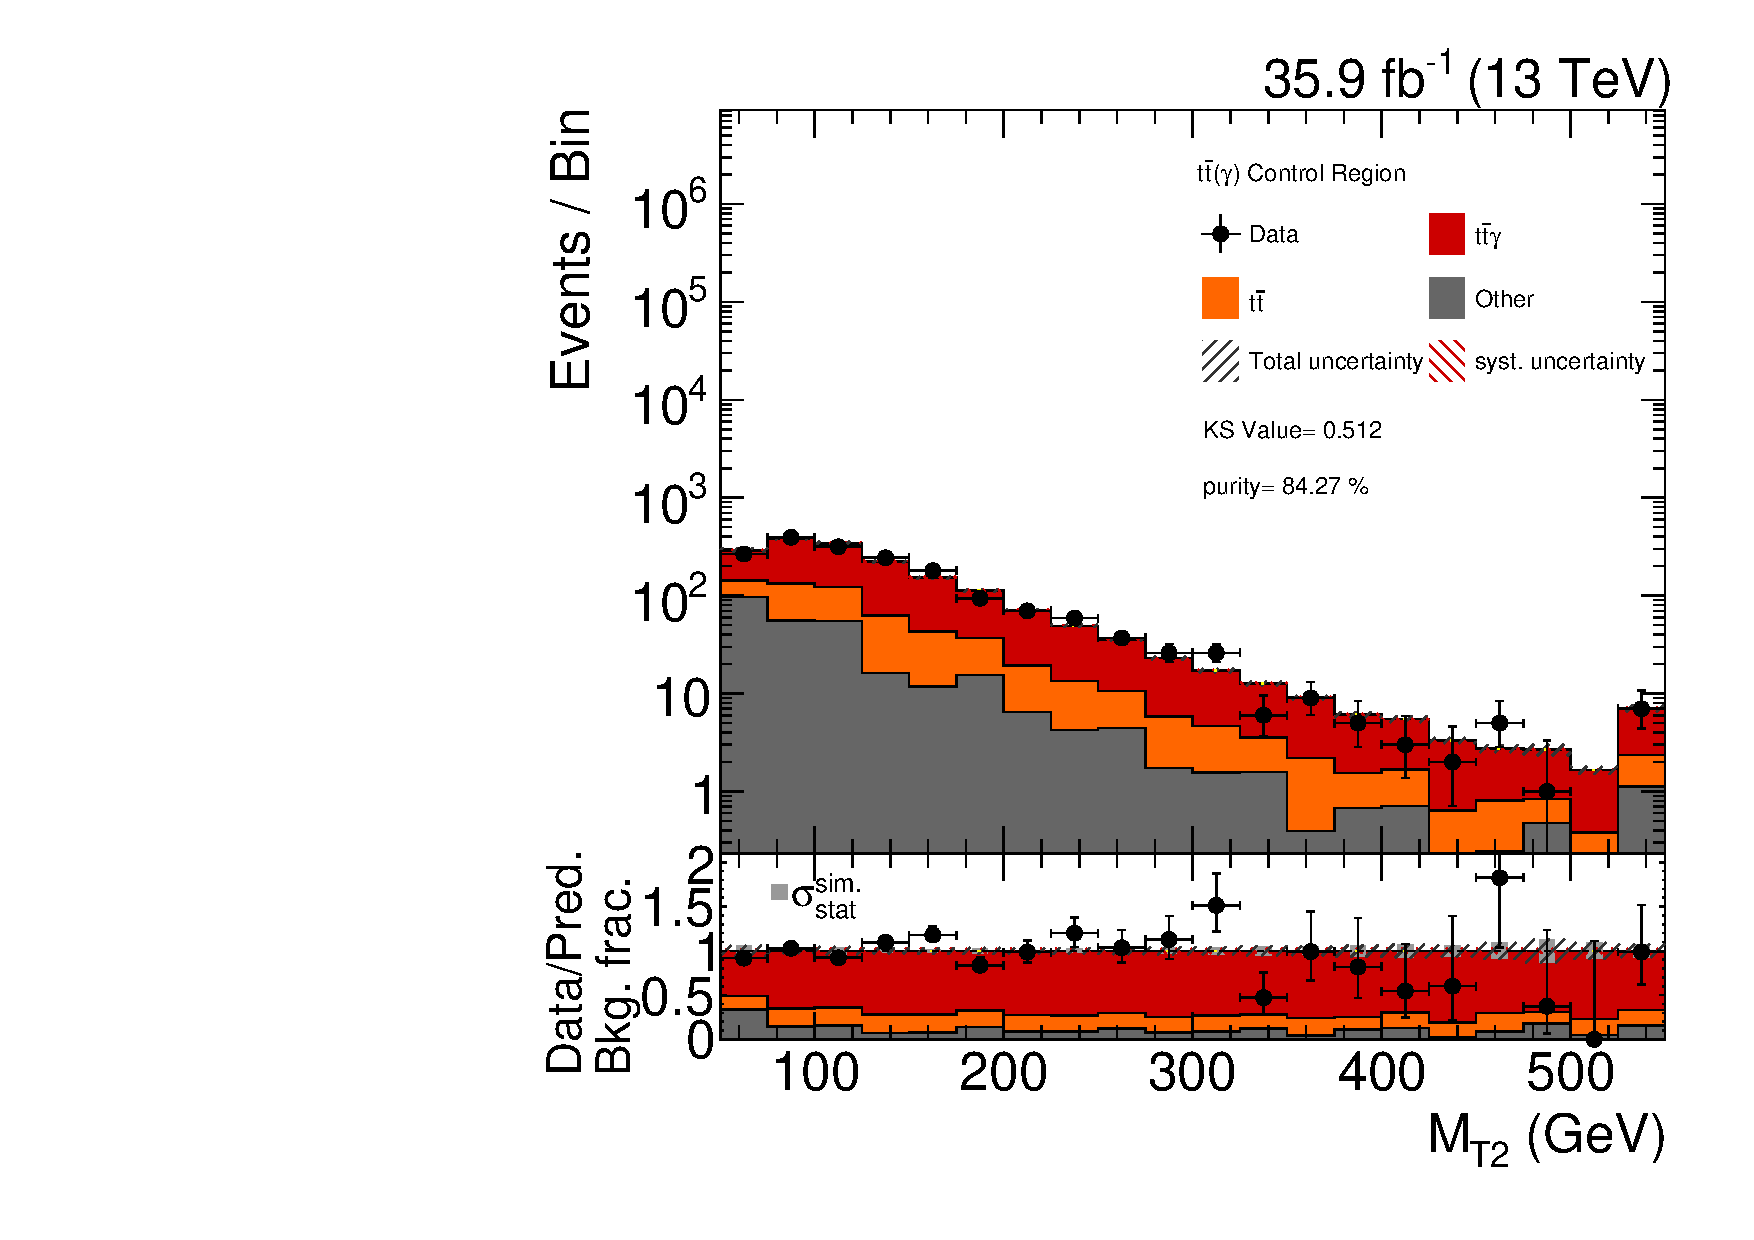
\includegraphics[width=\pairwidth]{figures/plots_CR_tt/CRTT_EM_nom_mt2_log}
 \caption{Comparisons between data and rescaled simulation in the $\ttbar(\PGg)$ CR in the $\ptmiss$ and $\mtTwo$ distribution. Below each plot, a ratio between data and prediction is shown. The uncertainty bands correspond to the systematic (red) and total uncertainty (gray). In addition, in the ratio plot the relative compostion of the backgrounds is visualized. KS-values for the performed Kolmogorov-Smirvov test are also quoted.}
 \label{fig:CRTT}
\end{figure}
In order to study a possible bias of observables not well modeled within the simulation, additional cross checks are performed. Similar to the SF calculation in the integral method, SFs are determined via $\chi^2$ minimization in the same CRs. Albeit this method is somewhat correlated to the method explained above, it enables the possibility to study influences of different distributions in different binnings. Therefore, $\alpha_{\ttbar(\PGg)}$ was varied in a range in small steps of $0.01$ for each binning and distribution, and for every iteration the simulation was scaled and the $\chi^2$ was calculated, which is defined as:
\begin{equation}
 \chi^2=\sum_i^{N_{bins}} \frac{\left(N_{i,bin}^{obs}-N_{i,bin}^{predicted}\right)^2}{N_{i,bin}^{predicted}}.
\end{equation}
The best fit value is determined to be at the minimum of the $\chi^2$ distribution, which is obtained by fitting a polynomial of fourth grade to the measured points. The uncertainty of the $\chi^2$-fit method, that is also of statistical origin, is calculated by taking the difference between the best fit value and the values, where $\chi^2=\chi^2_{BestFit}+1$. An example fit in the $\ptmiss$ distribution is shown in \refFig{fig:chiTT} left. The number of degrees of freedom (ndf) is given by the number of bins used to obtain the $\chi^2$ distribution reduced by the number of parameters that are being optimized. The only free parameter is $\alpha_{\ttbar(\PGg)}$, so $ndf$ equals the bin number subtracted by one. The resulting curves are smooth, indicating a proper performance of the fit. A comparison of all obtained SFs for the different setups and the SF obtained by the integral method is shown in \refFig{fig:chiTT} right. No significant deviation can be observed, and all SFs are in agreement within each other. Hence, the scaling of the $\ttbar(\PGg)$ background seems stable and well described in the CR.
\begin{figure}[tbp]
 \centering
 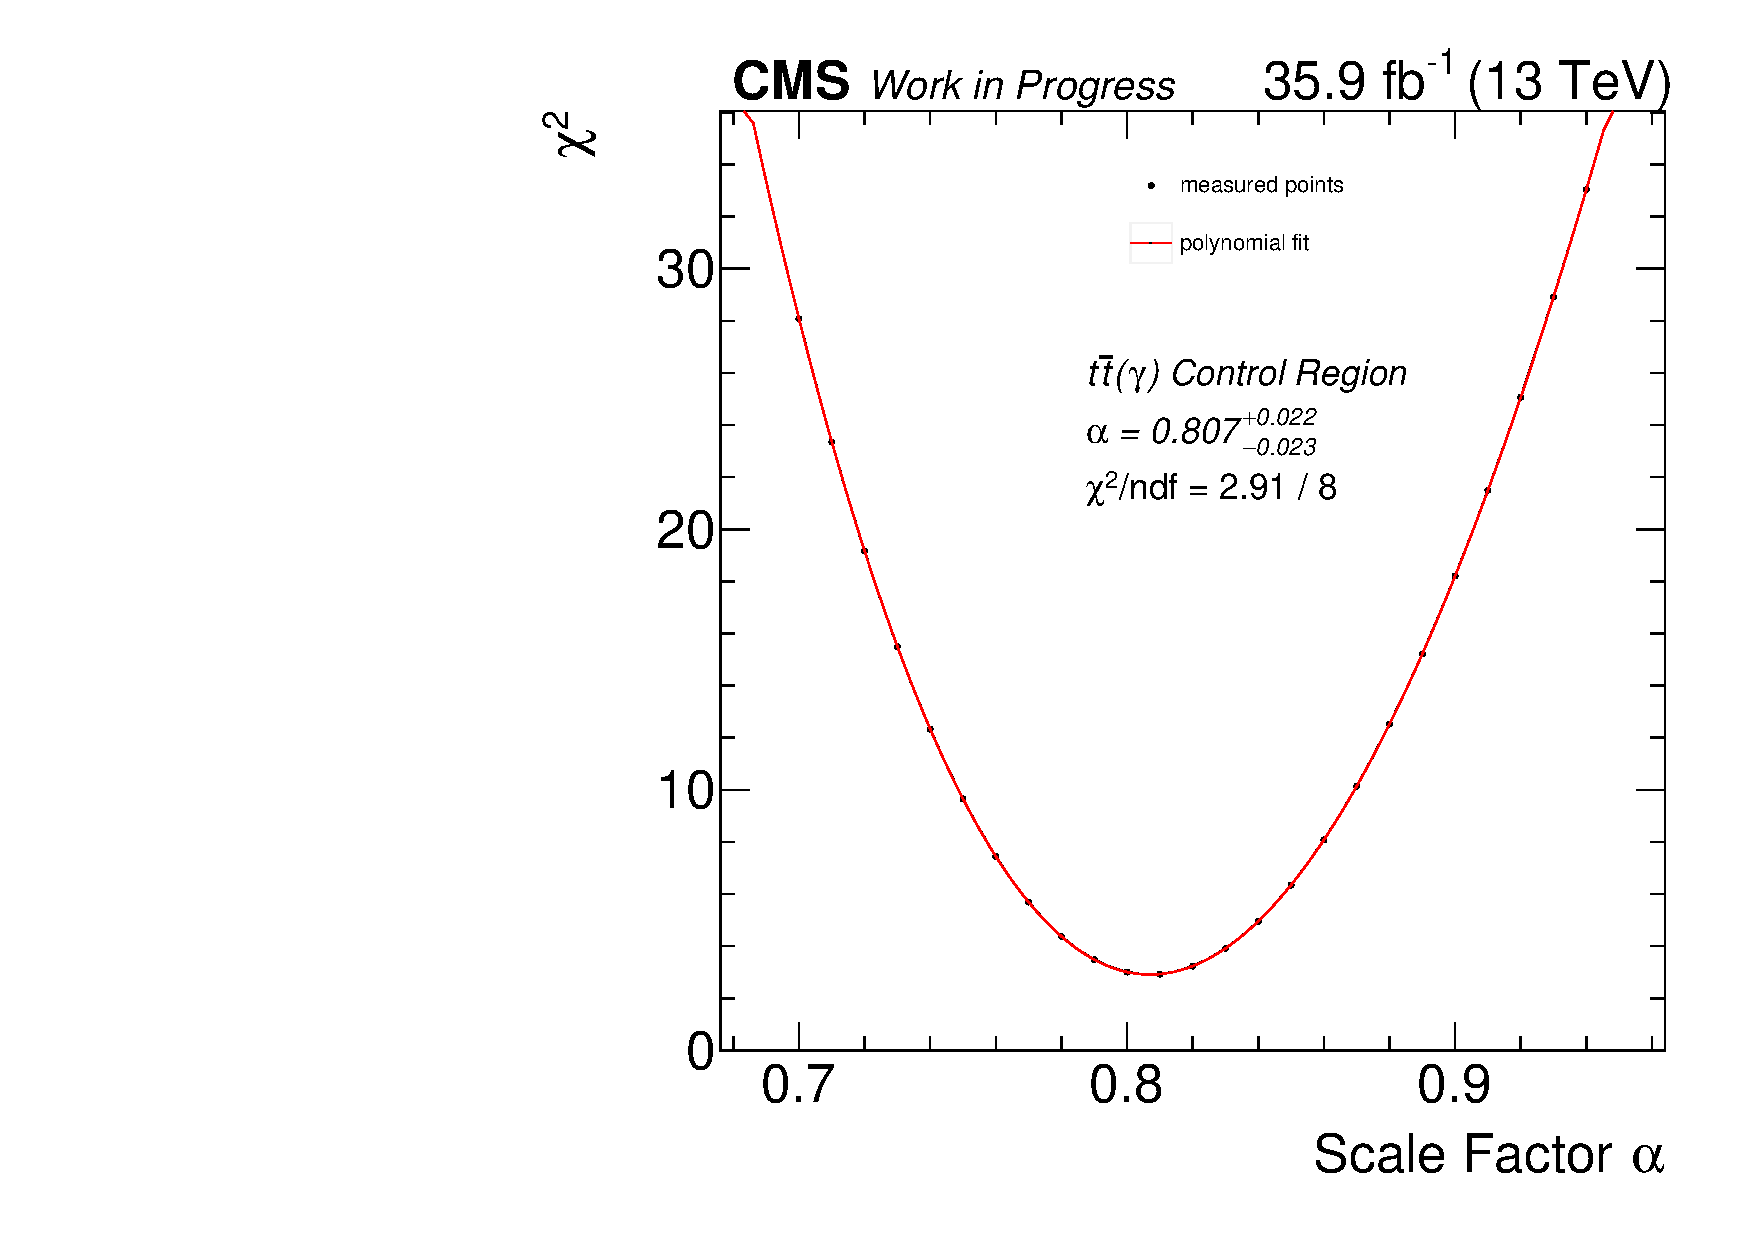
\includegraphics[width=\pairwidth]{figures/plots_CR/chi/TT_met}
 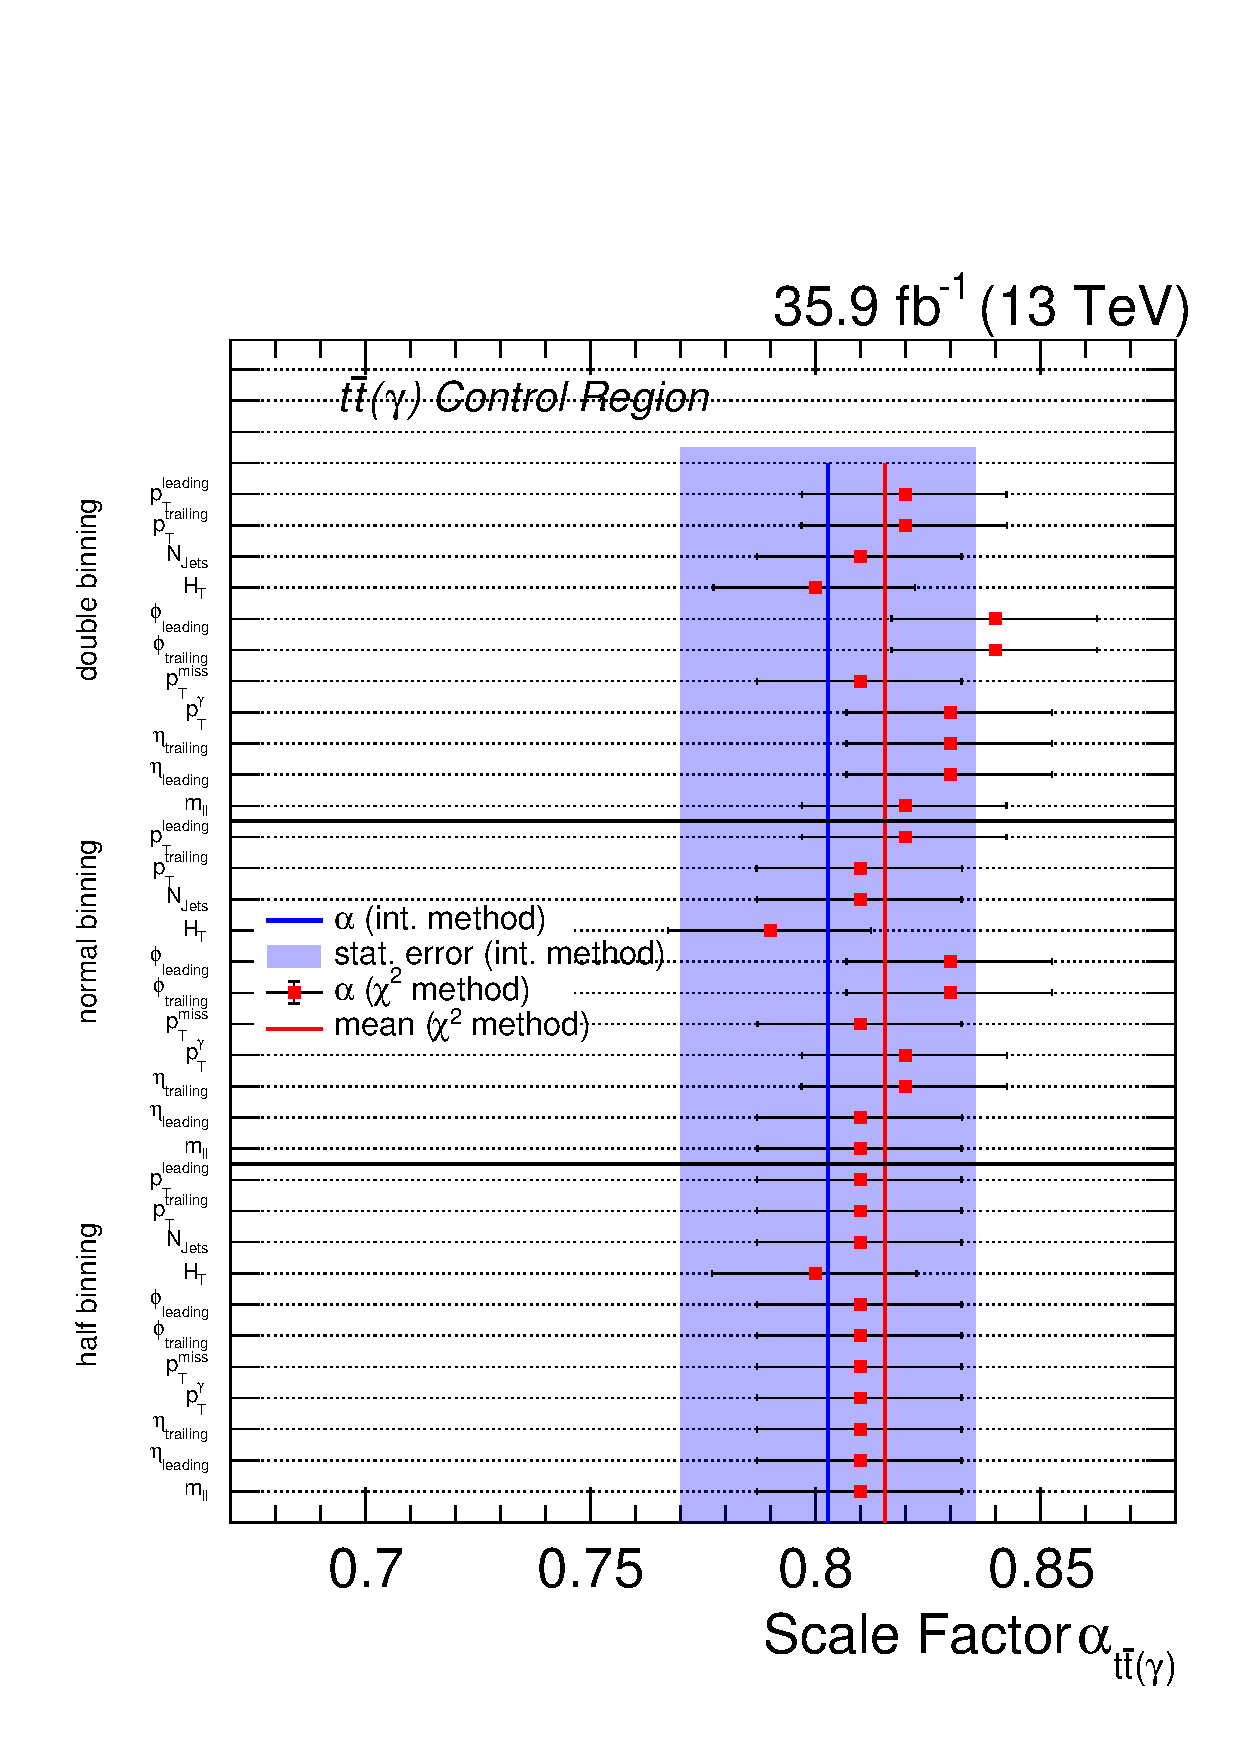
\includegraphics[width=\pairwidth]{figures/plots_CR/chi/TT_Compare}
 \caption{Example $\chi^2$ fit in the $\ttbar(\PGg)$ CR in the $\ptmiss$ distribution (left) with the polynomial fit. All fit results compared with the SF obtained from the integral method in different binnings and variables (right.)}
 \label{fig:chiTT}
\end{figure}

\subsubsection*{Further studies}
Since the $\ttbar(\PGg)$ background is the most dominating one, further studies are realized in which the underlying MC simulation samples and their combination are examined. Hence, different overlap removal procedures, see \refSec{sec:overlap}, and different available cross sections are used, while the fit procedure itself is varied. In addition, available corrections to improve the modeling of jet radiation in the initial state, and corrections to enhance the description of the top quark $\pt$ distribution, that are used both to correct the LO samples and the samples that are generated with \POWHEG (see~\refSec{sec:Simulation}), are applied in different combinations. The used fit methods include a $\chi^2$-template fit, where the ratio between the fractions of the $\ttbar$ and $\ttbar\PGg$ simulation is left free as an additional parameter, and a fit where only the $\ttbar\PGg$ simulation is made use of. Eventually, no substantial differences are observed, and the best performance and stability is provided by the initial approach explained above in detail.



\subsection{Drell-Yan and $\PZ\PGg$ diboson production}
Although the Drell-Yan and dibosonic $\PZ\PGg$ background is admittedly small in the two SR bins, its contribution is the fourth largest. Hence, it needs to be assured, that the background is modeled well. As in the case of the $\ttbar(\PGg)$ background, it is composited of two major parts, the Drell-Yan process, where quarks annihilate to off shellphotons or Z bosons and generate leptons in their decays, and the diboson production of $\PZ\PGg$ pairs. The integral method as explained above is used to determine the SF $\alpha_{DY/\PZ(\PGg)}$ in the dedicated CR defined in \refSec{sec:CR}. The relevant event yields are quoted in \refTab{tab:CRDY}, and the resulting SF is stated in \refEq{eq:AlphaDY}. With a purity of about $99\%$, and a total event count that large, a precise SF determination is feasible, as can be concluded also from the small statistical uncertainty of $\approx1\%$. The agreement between simulation and data is very good, even before application of $\alpha_{DY/\PZ(\PGg)}$, since it euquals nearly unity. The post-scaling distributions of $\ptmiss$ and $\mtTwo$ are shown in \refFig{fig:CRDY}. They show overall a good agreement, only in the high $\mtTwo$ region there are some fluctuations due to the limited statistics being present both in data and simulation.
% Further distributions are investigated, that can be found in the appendix in \refFig{fig_app}.
The same cross checks as for the $\ttbar(\PGg)$ background are made, including the Kolmogorov-Smirnov tests, and the additional $\chi^2$-fits with variable bin size in different observables.
All in all the KS-values indicate a very good matching between predicted and observed shape, albeit the Kolmogorov-Smirnov test provides a very small KS value for the consistency between the $\ptmiss$ distributions. But, this is mainly due to the high statistics in data and therefore a higher absolute discrepancy, contradicting with the lower statistics in simulation, leading to larger fluctuations. These discrepancy is not visible in the ratio shown under the plot.\\
\begin{table}[tbp]
 \centering
 \caption{Yields in the DY/$\PZ(\PGg)$ CR for the pure simulation and measured data.}
 \label{tab:CRDY}
 \begin{tabular}{llll}
  
  process   & raw simulation & simulation & data                   \\\hline
  Drell-Yan & 11710          & 13008.53   &                        \\
  $\PZ\PGg$ & 170161         & 22692.88   &                        \\\hline\hline
  sum       & 181871         & 35701.41   & \multirow{2}{*}{38419} \\
  other     & 87337          & 377.02     &                        
 \end{tabular}
\end{table}
\begin{equation}\label{eq:AlphaDY}
 \alpha_{DY/\PZ(\PGg)}=1.066 \pm 0.001 (stat.) [\hat{=}0.87\%].
\end{equation}

\begin{figure}[tbp]
 \centering
 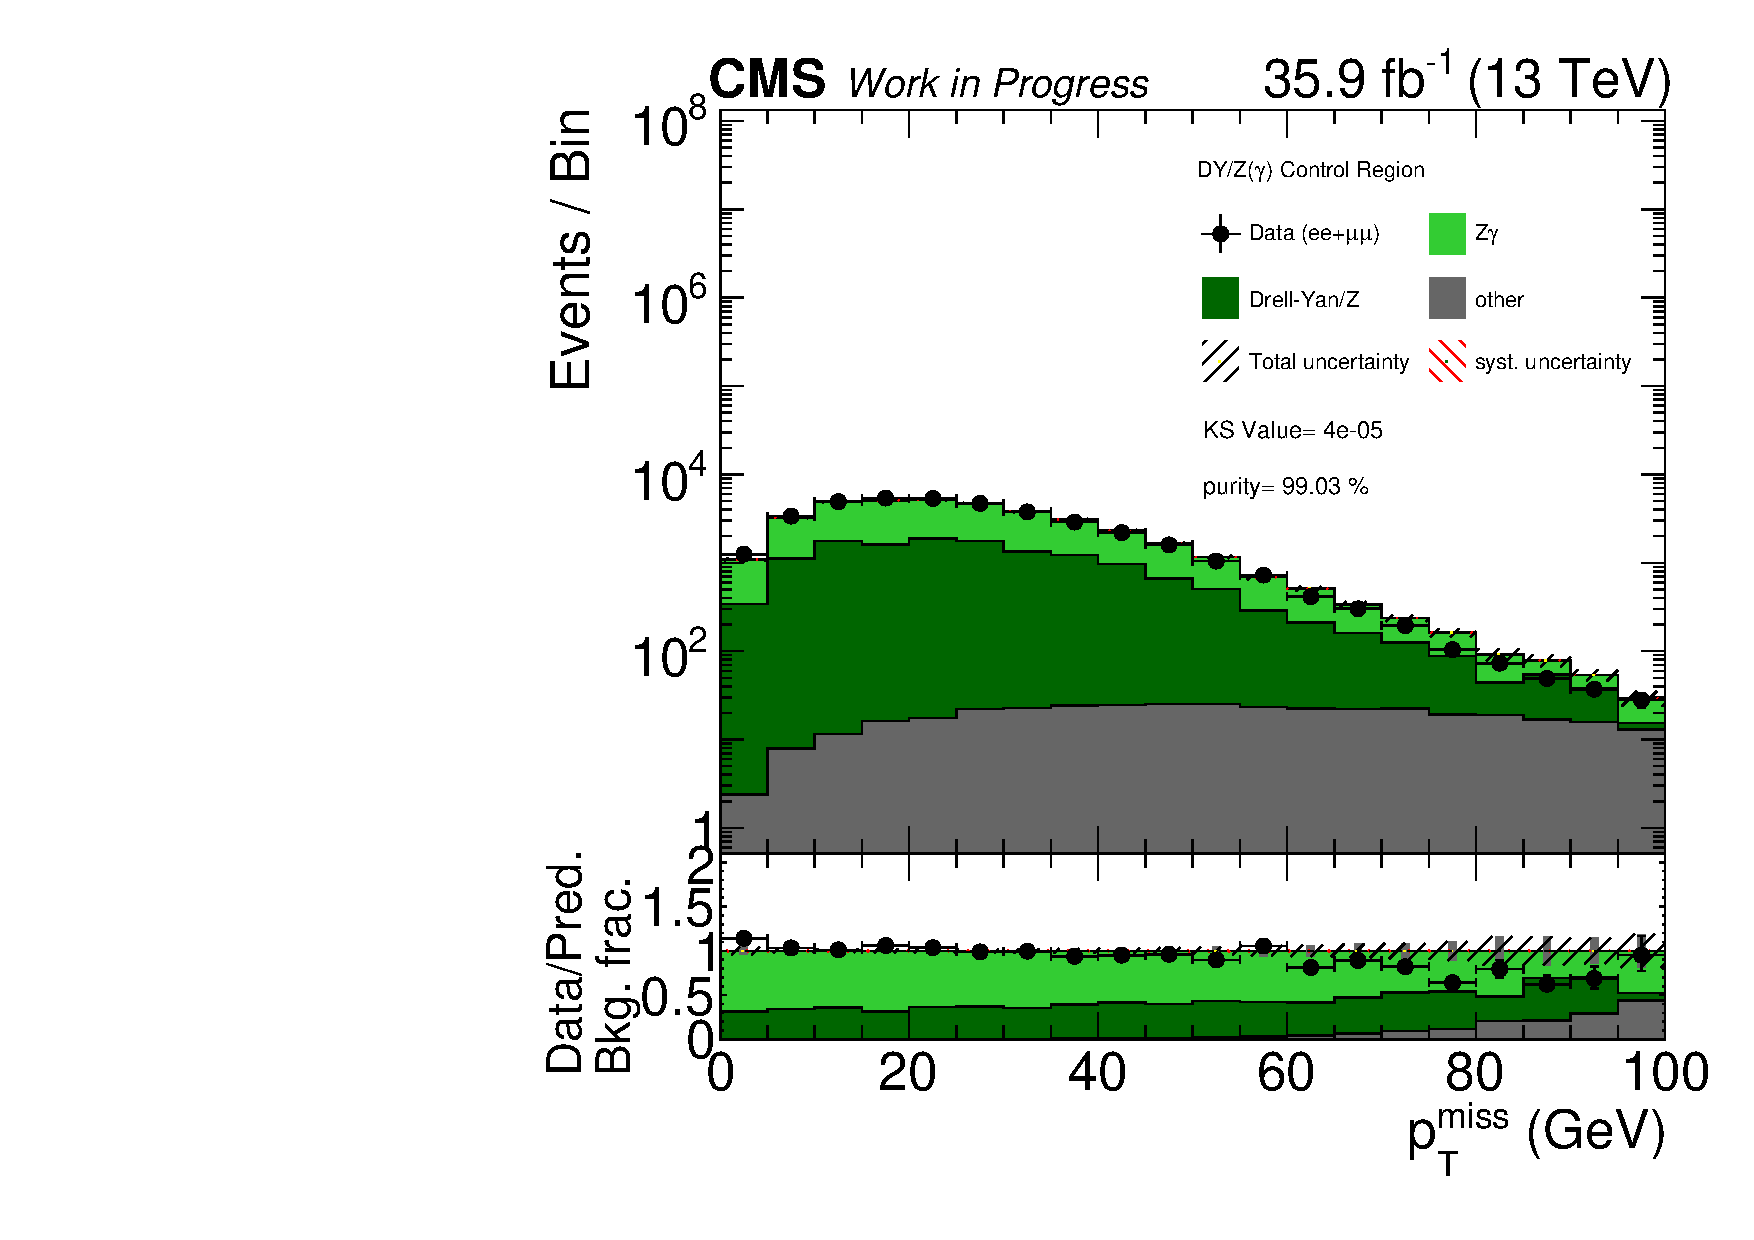
\includegraphics[width=\pairwidth]{figures/plots_CR_dy/CRDY_LL_nom_met_log}
 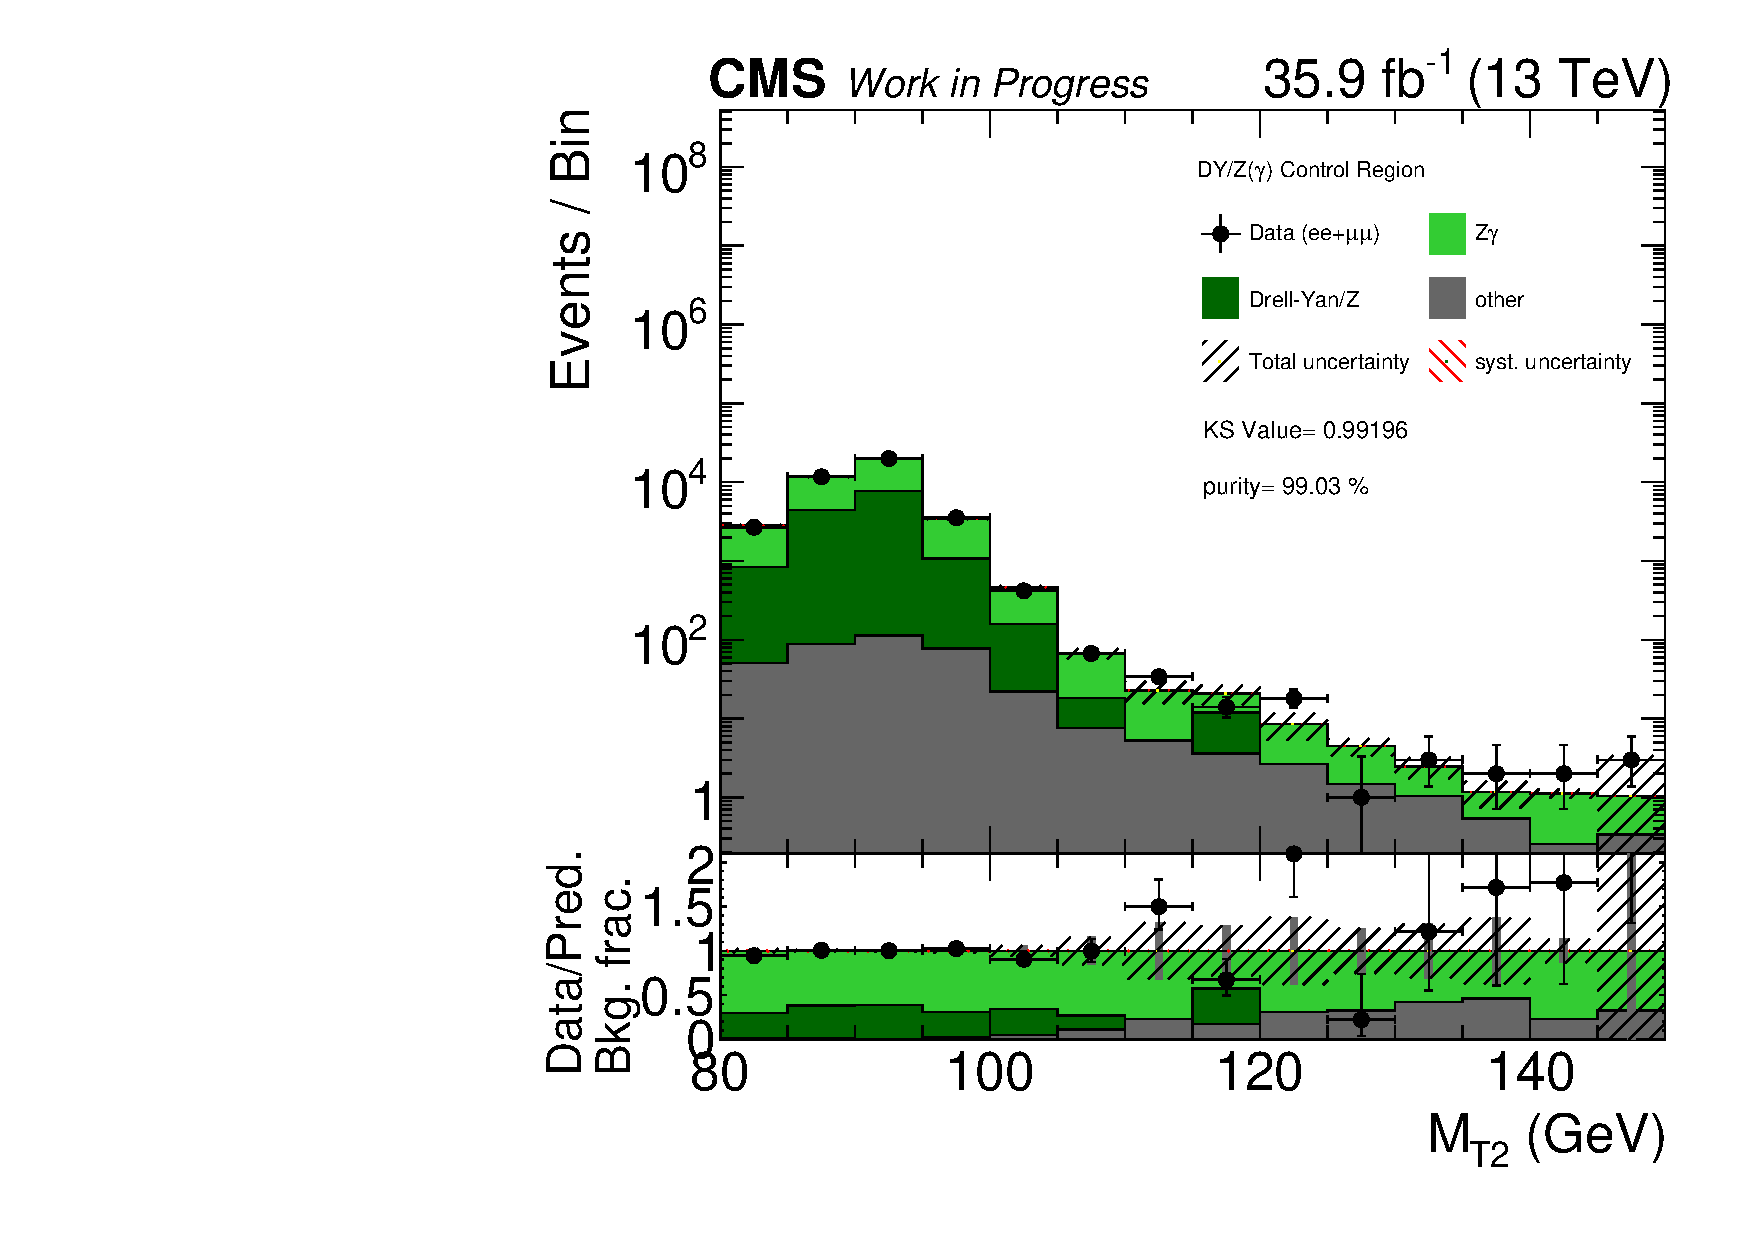
\includegraphics[width=\pairwidth]{figures/plots_CR_dy/CRDY_LL_nom_mt2_log}
 \caption{Comparisons between data and rescaled simulation in the DY/$\PZ(\PGg)$ CR in the $\ptmiss$ and $\mtTwo$ distribution. Below each plot, a ratio between data and prediction is shown. The uncertainty bands correspond to the systematic (red) and total uncertainty (gray). In addition, in the ratio plot the relative compostion of the backgrounds is visualized. KS-values for the performed Kolmogorov-Smirvov test alre also quoted.}
 \label{fig:CRDY}
\end{figure}
The $\chi^2$-fit studies, shown in \refFig{fig:chiDY} together with an example fit in the $\ptmiss$ distribution, show excellent agreement over all variations. Hence, the background prediction seems to work fine also in the DY/$\PZ(\PGg)$ CR.

\begin{figure}[tbp]
 \centering
 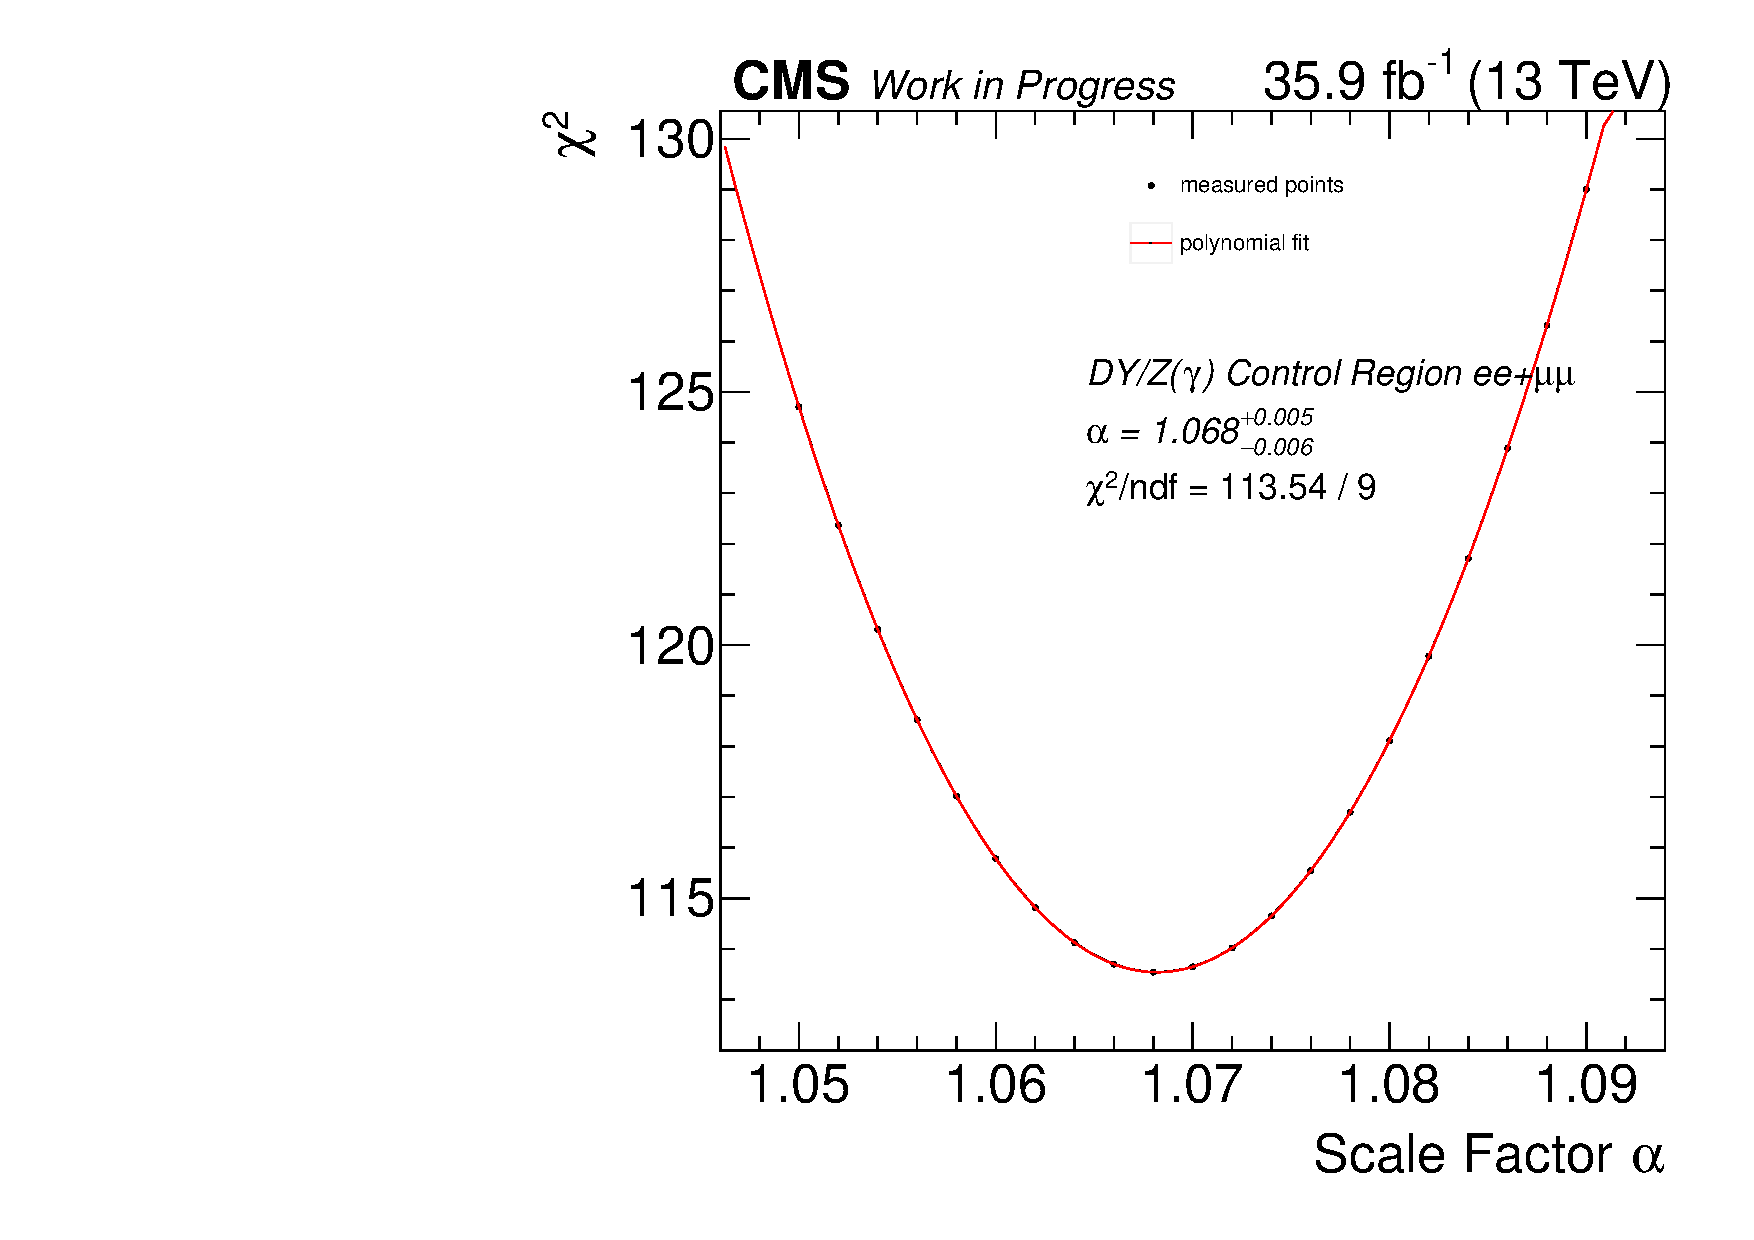
\includegraphics[width=\pairwidth]{figures/plots_CR/chi/DY_LL_met}
 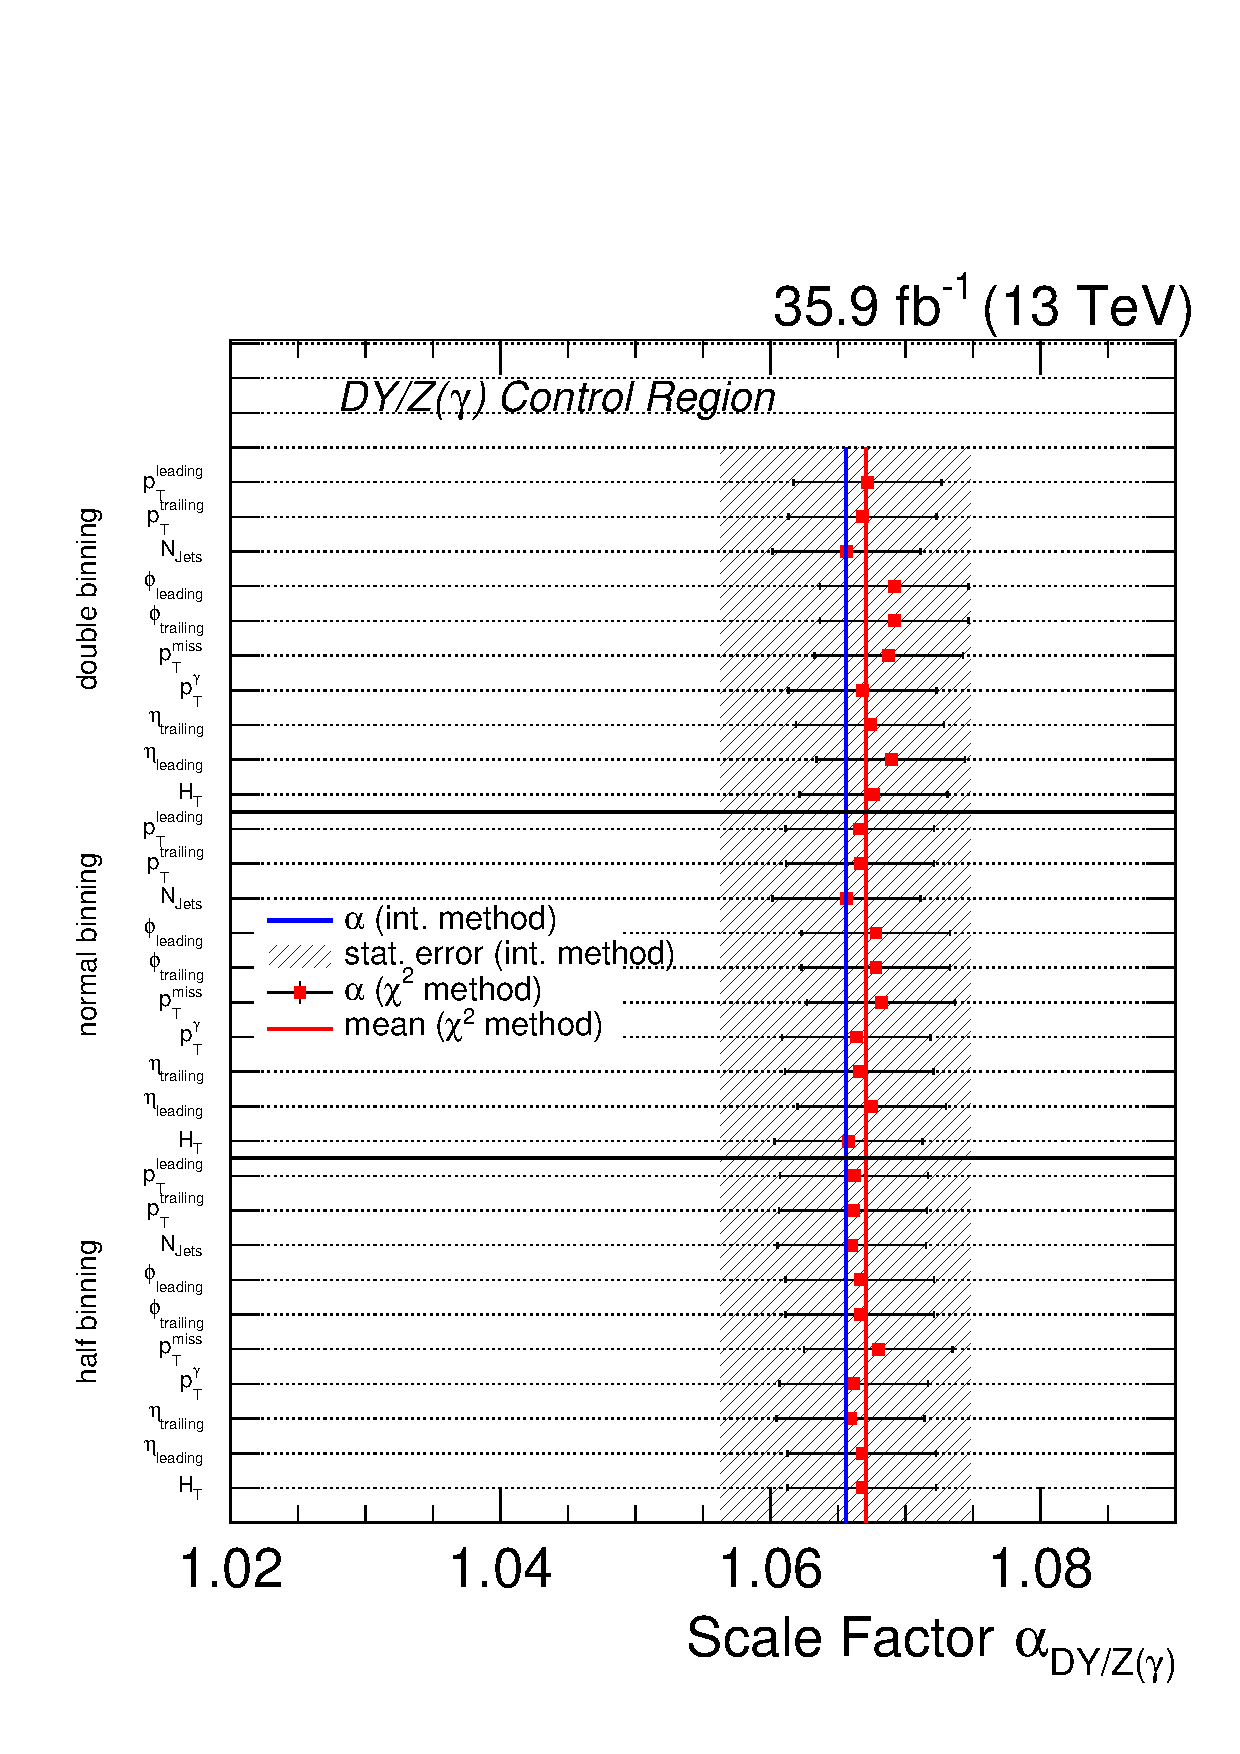
\includegraphics[width=\pairwidth]{figures/plots_CR/chi/DY_CompareLL}
 \caption{Example $\chi^2$ fit in the DY/$\PZ(\PGg)$ CR in the $\ptmiss$ distribution (left) with the polynomial fit. All fit results compared with the SF obtained from the integral method in different binnings and variables (right.)}
 \label{fig:chiDY}
\end{figure}

\subsection{$\PW\PZ$ diboson production}
The diboson production of $\PW\PZ$ pairs is the second important background contribution for this analysis. It is also tuned to agree with the measurement in the $\PW\PZ$ CR, while the SF $\alpha_{\PW\PZ}$ is calculated with the integral method. The expected purity of selected $\PW\PZ$ events in this CR is about $84\%$, and the total event yields given in \refTab{tab:CRWZ} point out, that the number of events is sufficient to determine a SF with adequate precision.
\begin{table}[tbp]
 \centering
 \caption{Yields in the $\PW\PZ$ CR for the pure simulation and measured data.}
 \label{tab:CRWZ}
 \begin{tabular}{llll}
  process  & raw simulation & simulation & data                  \\\hline
  $\PW\PZ$ & 113744         & 895.74     &                       \\\hline\hline
  sum      & 113744         & 895.74     & \multirow{2}{*}{1193} \\
  other    & 93914          & 173.47     &                       
 \end{tabular}
\end{table}
The agreement beforehand is also very good, although this background is a higher order process and is therefore simulated at NLO, see \refSec{sec:Simulation}, which includes several complicated effects the event generator needs to handle properly. The SF $\alpha_{DY/\PZ(\PGg)}$ is determined to be
\begin{equation}\label{eq:AlphaWZ}
 \alpha_{\PW\PZ}=1.138 \pm 0.037 (stat.) [\hat{=}3.23\%],
\end{equation}
which indicates that usage of NNLO cross sections for the $\PW\PZ$ samples is nearly sufficient enough to describe the background. Of course higher order effects can lead to higher cross sections, thus it is not unexpected to obtain a SF varying $\approx12\%$ from unity. Resulting distributions of the description of the $\ptmiss$ and $\mtTwo$ variables are shown in \refFig{fig:CRWZ}. As can be seen, the predicted shape is in consistency over the whole range with the observed data, also in the very high $\ptmiss$ and $\mtTwo$ regime. This is further confirmed by the additional cross checks, that are also realized in the other two CRs described above. The KS-values close to one strengthen the trust in the background estimation method.
% The comparison plots for other distributions can be found in the appendix in \refFig{fig:app_}.
\begin{figure}[tbp]
 \centering
 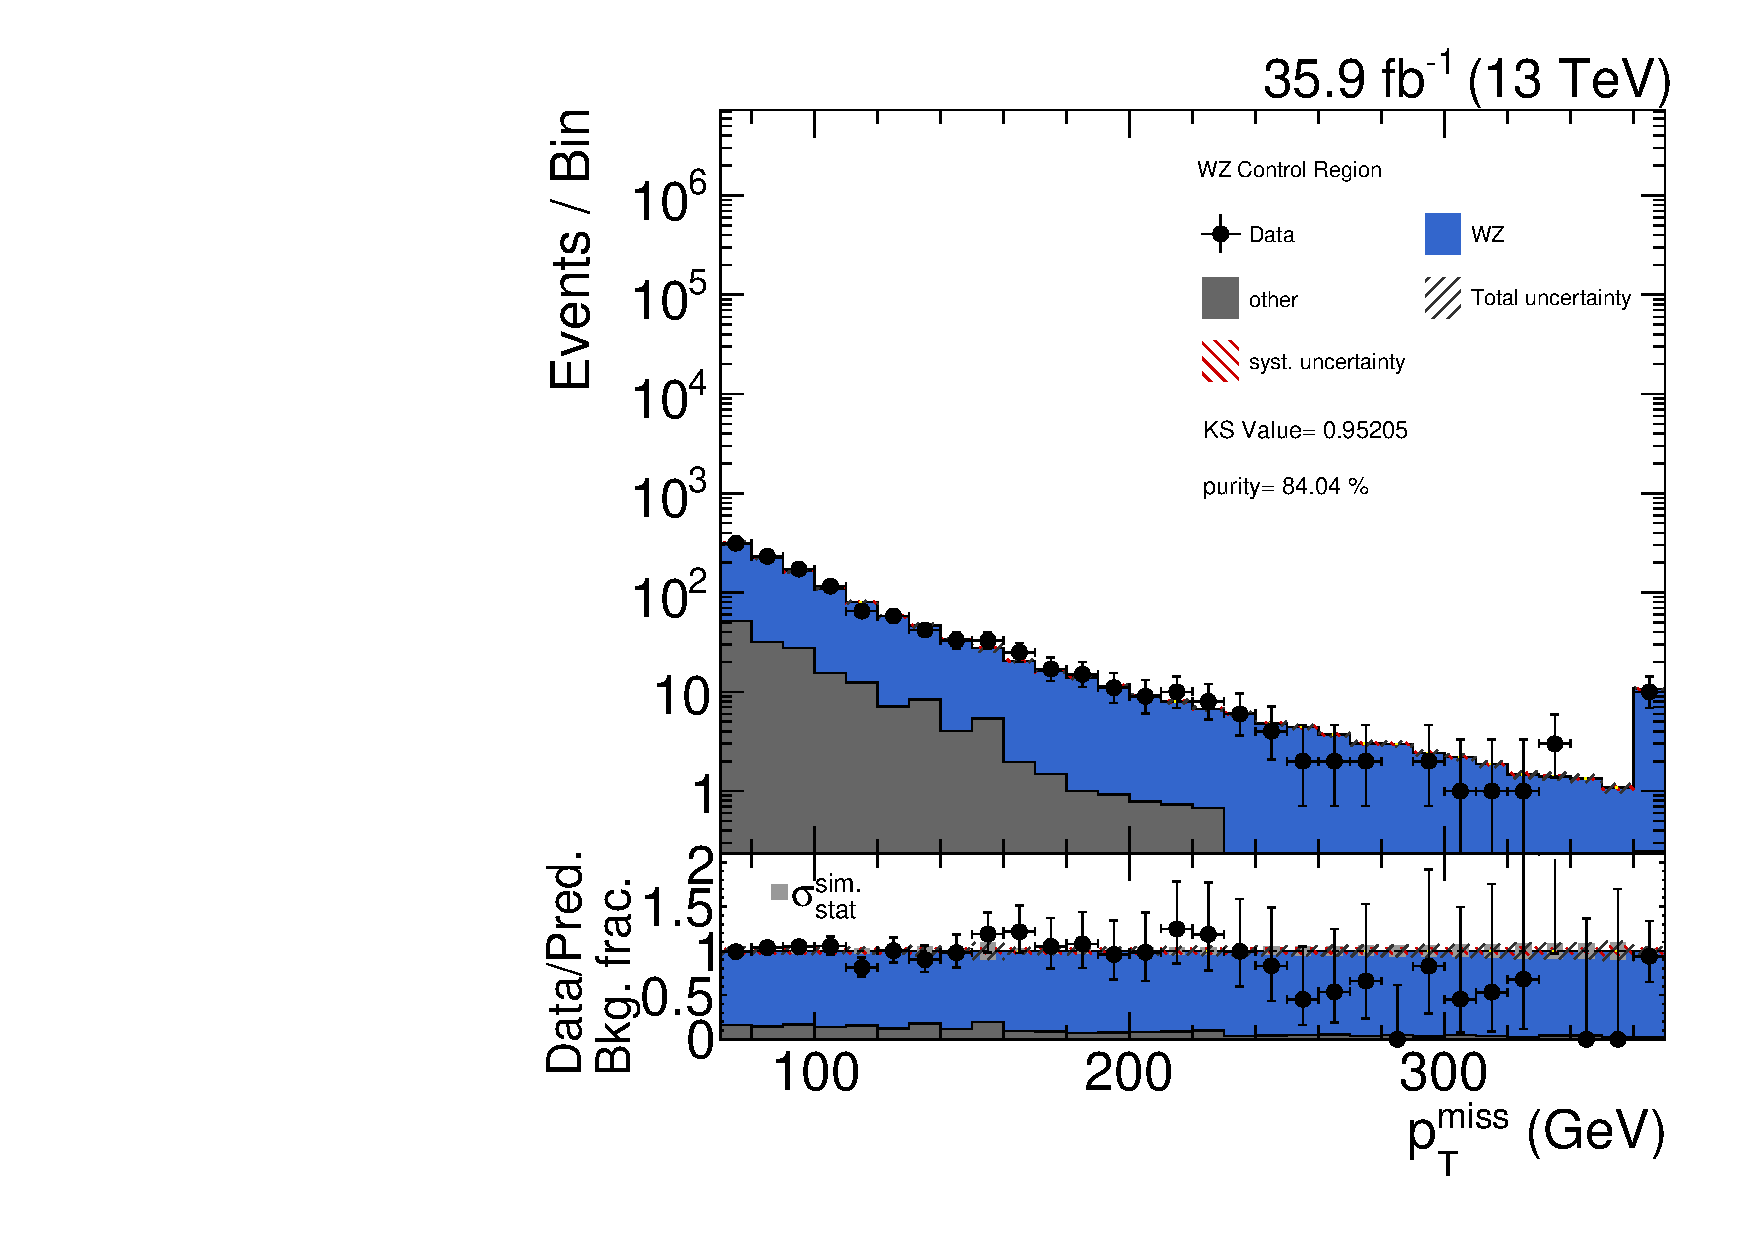
\includegraphics[width=\pairwidth]{figures/plots_CR_wz/CRWZ_LL_nom_met_log}
 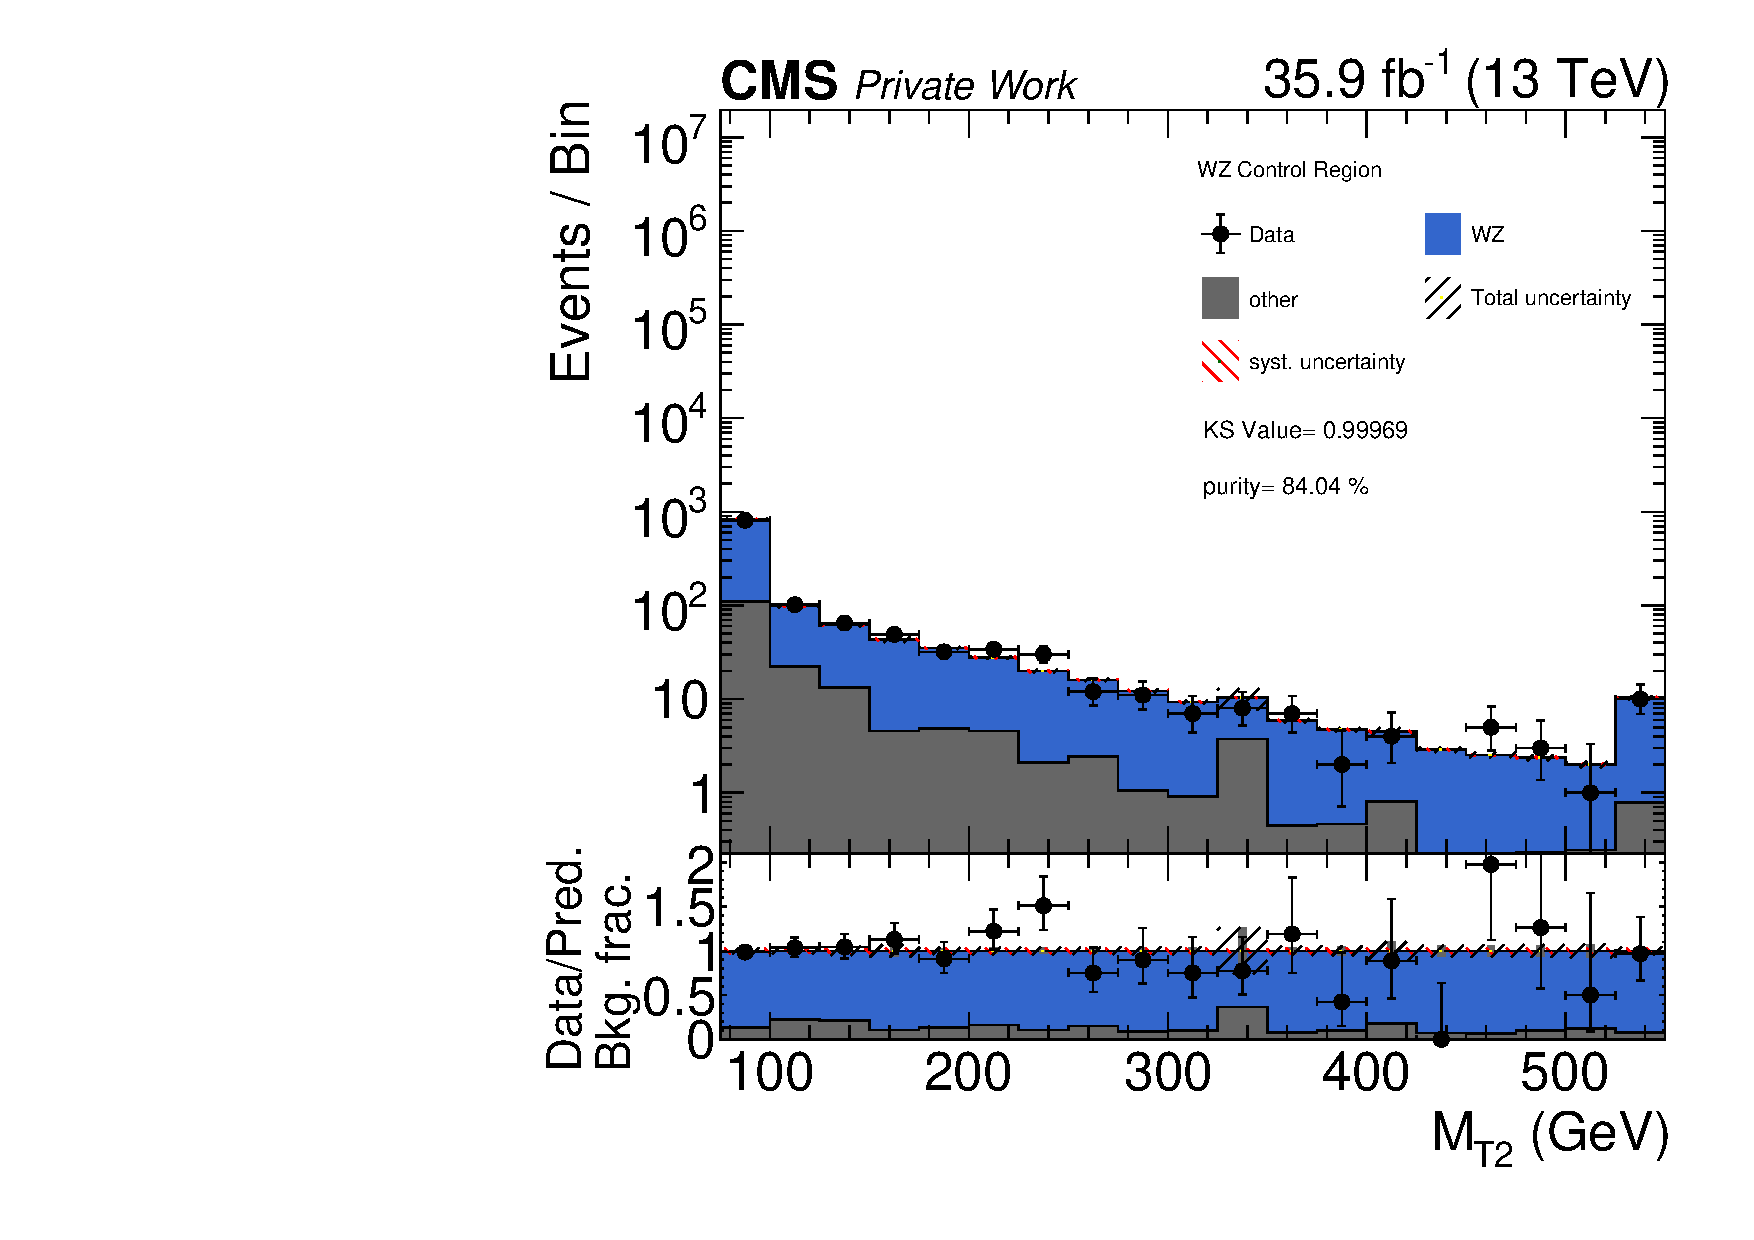
\includegraphics[width=\pairwidth]{figures/plots_CR_wz/CRWZ_LL_nom_mt2_log}
 \caption{Comparisons between data and rescaled simulation in the $\PW\PZ$ CR in the $\ptmiss$ and $\mtTwo$ distribution. Below each plot, a ratio between data and prediction is shown. The uncertainty bands correspond to the systematic (rand) and total uncertainty (gray). In addition, in the ratio plot the relative compostion of the backgrounds is visualized. KS-values for the performed Kolmogorov-Smirvov test alre also quoted.}
 \label{fig:CRWZ}
\end{figure}
The $\chi^2$-fit studies lead to the same outcome, the uncertainties seem to be well estimated and of statistical origin, since no large shape deviation can be observed in the performed fits, as can be seen in \refFig{fig:chiWZ} right. Each individual $\chi^2$-fit seems to behave properly, see \refFig{fig:chiWZ} left for an example in the $\ptmiss$ distribution.

\begin{figure}[tbp]
 \centering
 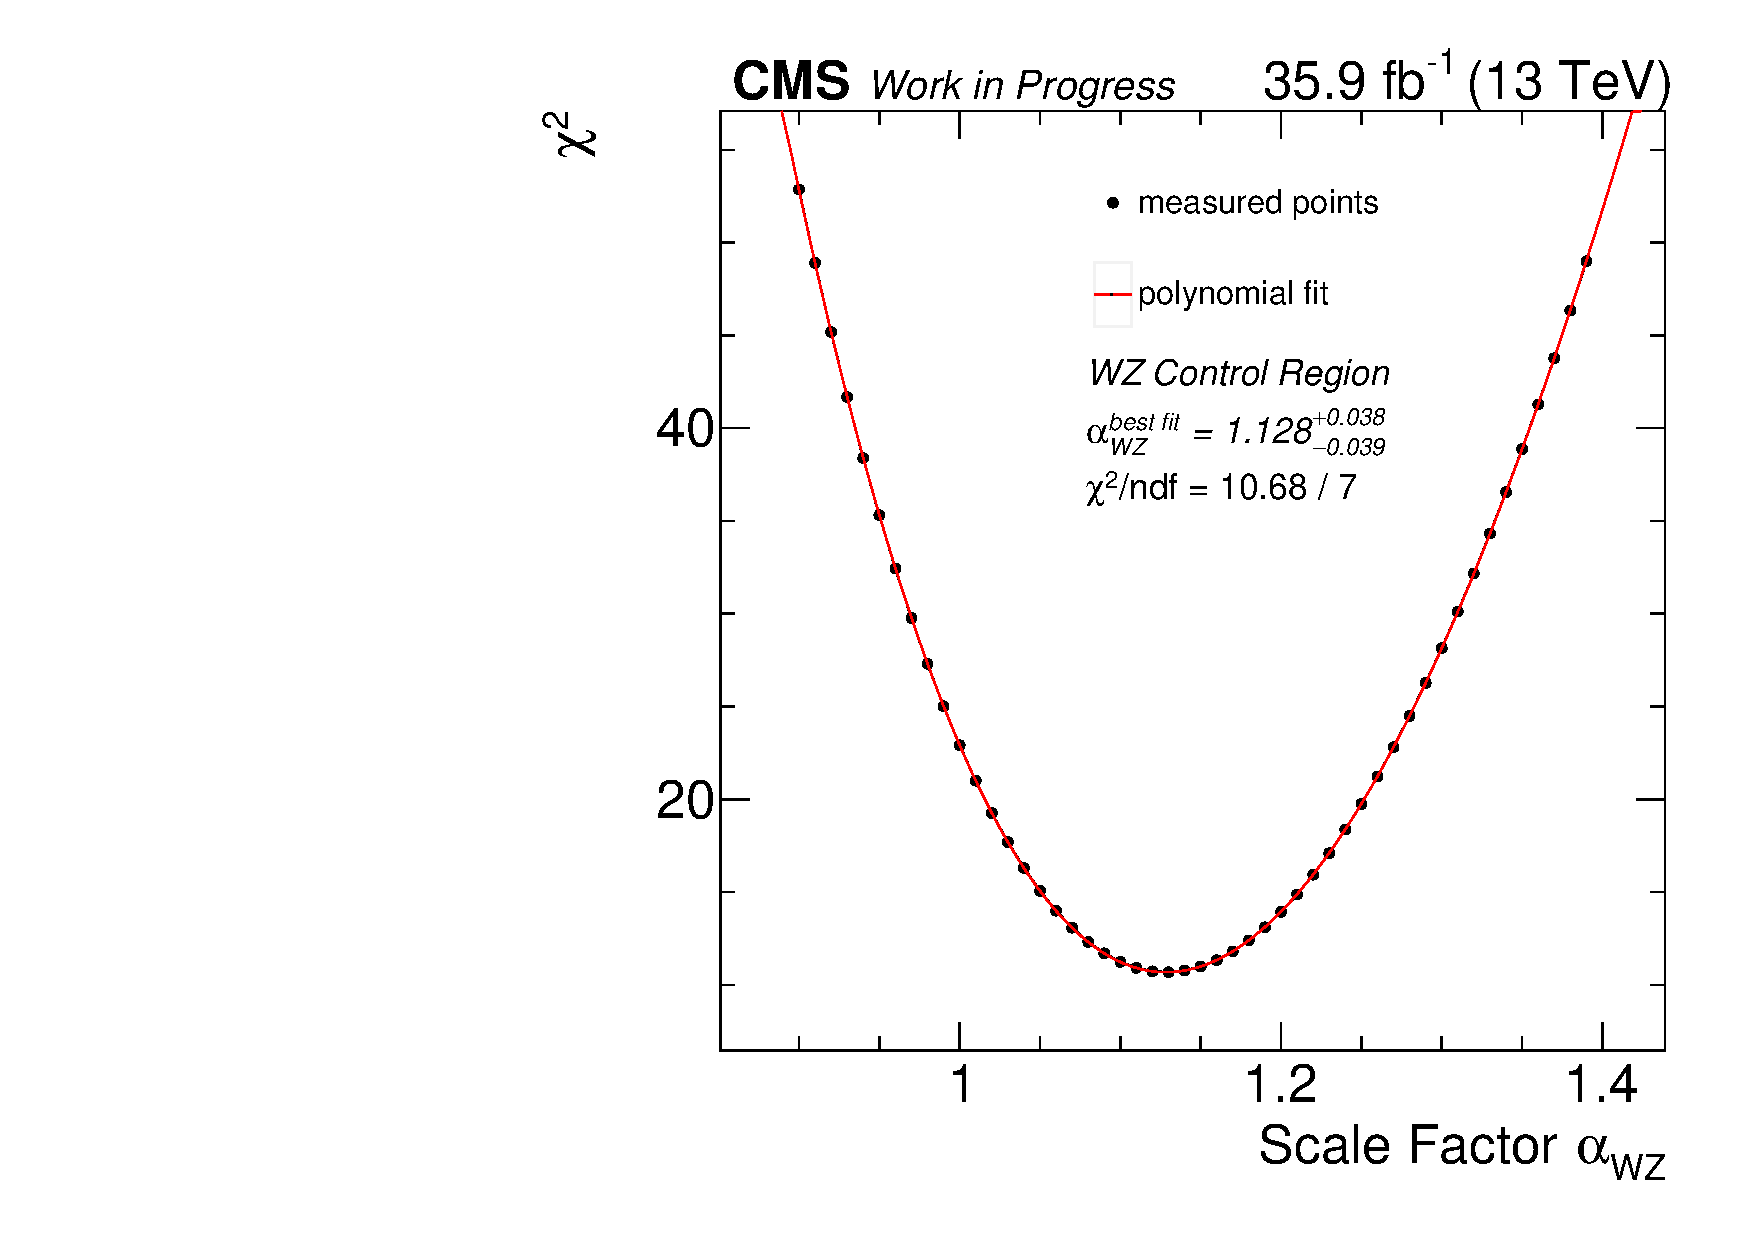
\includegraphics[width=\pairwidth]{figures/plots_CR/chi/WZ_met}
 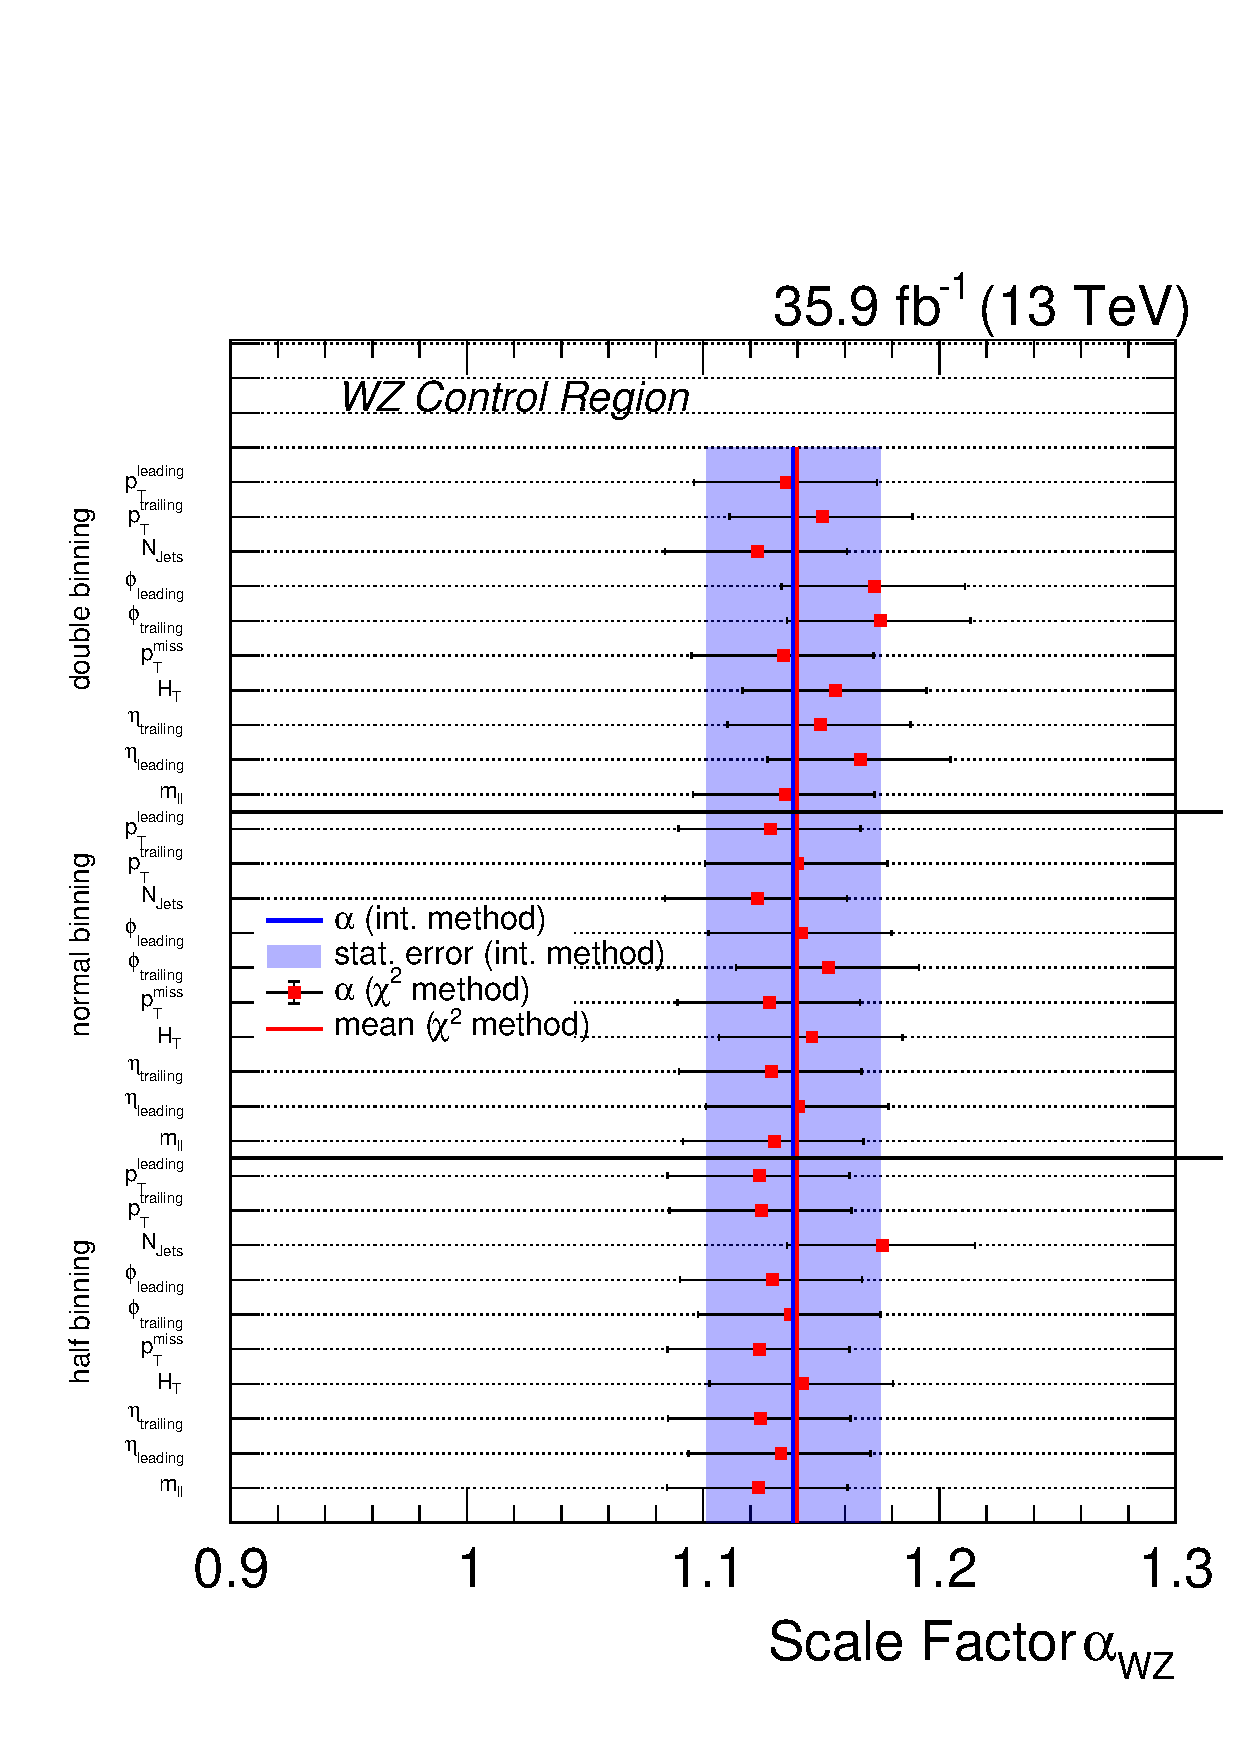
\includegraphics[width=\pairwidth]{figures/plots_CR/chi/WZ_Compare}
 \caption{Example $\chi^2$ fit in the $\PW\PZ$ CR in the $\ptmiss$ distribution (left) with the polynomial fit. All fit results compared with the SF obtained from the integral method in different binnings and variables (right.)}
 \label{fig:chiWZ}
\end{figure}


\subsection{$\PZ\PZ$ diboson production}
The last important and fourth biggest background contribution is $\PZ\PZ$ diboson production, where both Z bosons decay leptonically, one to charged leptons such as electrons or muons, and the other one to neutrinos. To simplify the construction of a dedicated CR, as explained in \refSec{sec:CR}, the assumption is made, that there is no difference for the generator to generate neutral or charged leptons. Only the detector response should differ. Therefore, $\PZ\PZ$ can be well estimated in a four lepton CR. A pure selection of $\PZ\PZ$ events can be established, although the statistics in data is quite low due to small cross section and the low branching fraction for the $\Z\to\ell\ell$ decay. Event counts are quoted in \refTab{tab:CRZZ}, with a selection purity of nearly $100\%$.
\begin{table}[tbp]
 \centering
 \caption{Yields in the $\PZ\PZ$ CR for the pure simulation and measured data.}
 \label{tab:CRZZ}
 \begin{tabular}{llll}
  
  process                 & raw simulation & simulation & data                 \\\hline
  $\PZ\PZ(\to2\ell2\Pgn)$ & 5              & 0.0005     &                      \\
  $\PZ\PZ(\to4\ell)$      & 459221         & 226.94     &                      \\\hline\hline
  sum                     & 459226         & 226.94     & \multirow{2}{*}{251} \\
  other                   & 74             & 1.48       &                      
 \end{tabular}
\end{table}
With the integral method applied, a SF $\alpha_{\PZ\PZ}$ stated in \refEq{eq:AlphaZZ} is determined, being relatively close to one.
\begin{equation}\label{eq:AlphaZZ}
 \alpha_{\PZ\PZ}=1.109 \pm 0.064 (stat.) [\hat{=}5.74\%].
\end{equation}
Post-fit distributions to show the good agreement in the $\ptmiss$ distribution and invariant dilepton mass distribution of the second Z boson can be found in \refFig{fig:CRZZ}. As mentioned, the precision is limited by the low statistics of the selected sample, but nevertheless is sufficient enough to establish a working background prediction. The shapes agree very well, as it is additionally indicated by the KS-values printed on the plots. The properties of the $\PZ\PZ\to4\ell$ processes does not allow to study the prediction in the high $\ptmiss$ regime, since only nongenuine $\ptmiss$ is produced. However, the agreement of distributions of the third and fourth leptons, such as $m_{\ell_3\ell_4}$, can be translated into the agreement of the $\ptmiss$ in the $\PZ\PZ\to2\ell2\PGn$ background, that is generated with the same event generator. There, also no
\begin{figure}[tbp]
 \centering
 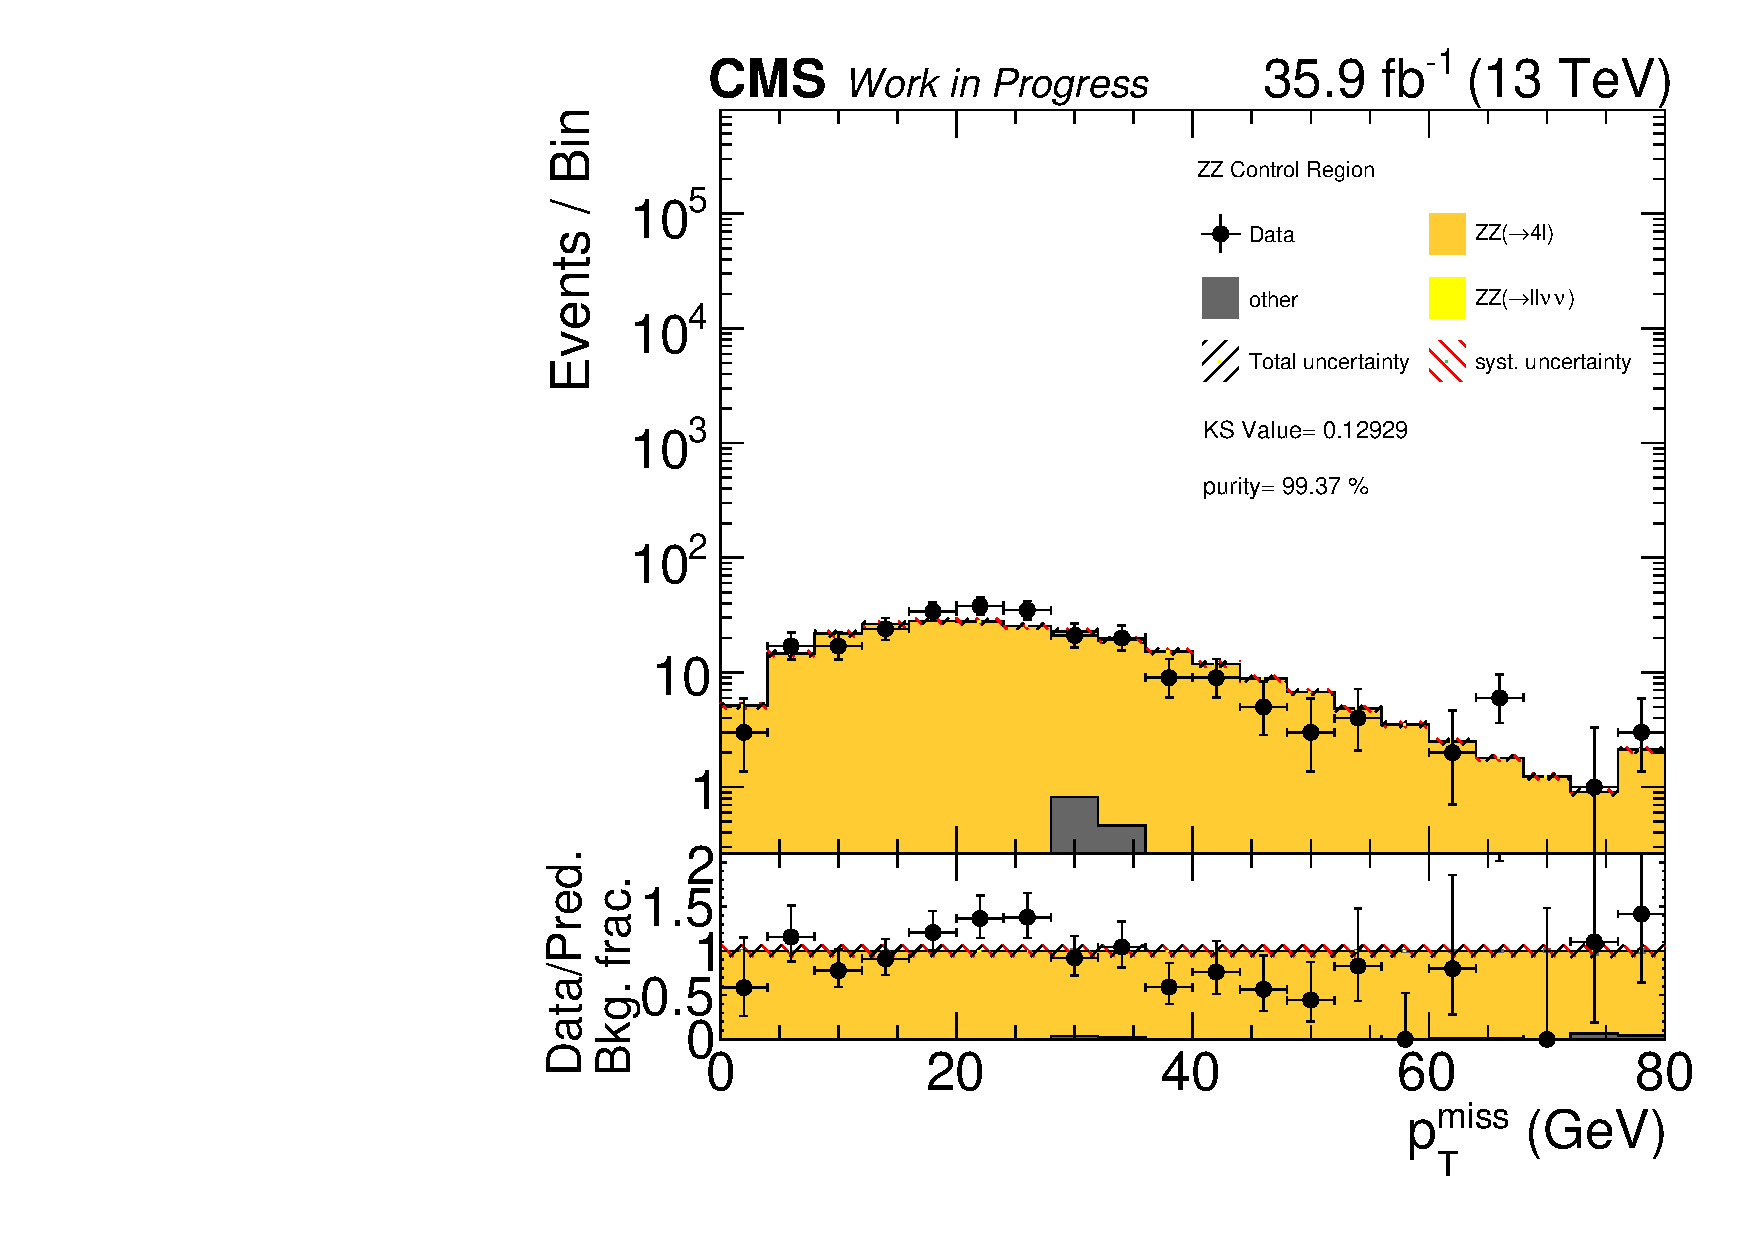
\includegraphics[width=\pairwidth]{figures/plots_CR_zz/CRZZ_LL_nom_met_log}
 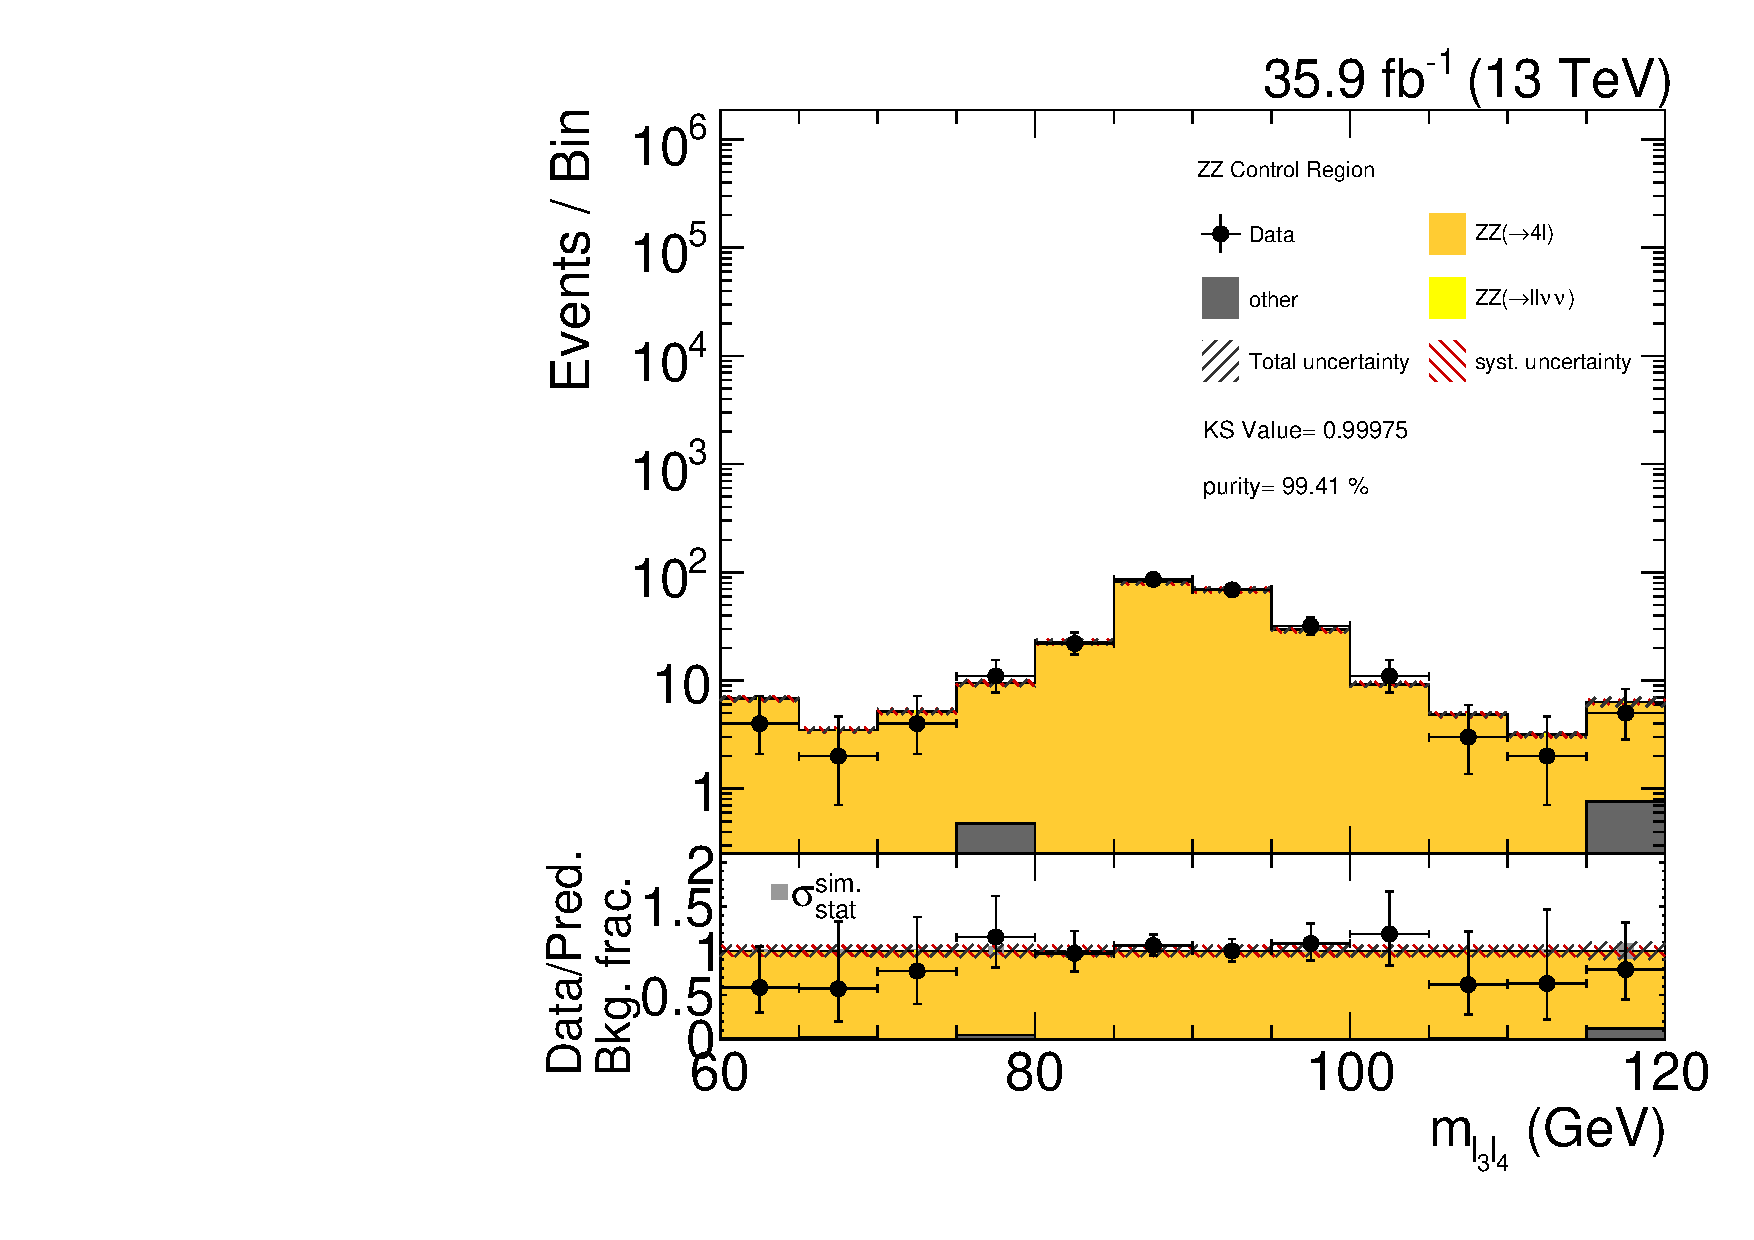
\includegraphics[width=\pairwidth]{figures/plots_CR_zz/CRZZ_LL_nom_m_ll2_log}
 \caption{Comparisons between data and rescaled simulation in the $\PZ\PZ$ CR in the $\ptmiss$ and $m_{\ell_3\ell_4}$ distribution. Below each plot, a ratio between data and prediction is shown. The uncertainty bands correspond to the systematic (red) and total uncertainty (gray). In addition, in the ratio plot the relative compostion of the backgrounds is visualized. KS-values for the performed Kolmogorov-Smirvov test alre also quoted.}
 \label{fig:CRZZ}
\end{figure}
The $\chi^2$-fit studies, see \refFig{fig:chiZZ}, are performed as for the other three background estimations discussed above, and yield the same conclusion, although some fluctuations in the choice of the variable or binning are present due to the lower total event count in the observed data. But, all in all also this background estimation method behaves properly.
\begin{figure}[tbp]
 \centering
 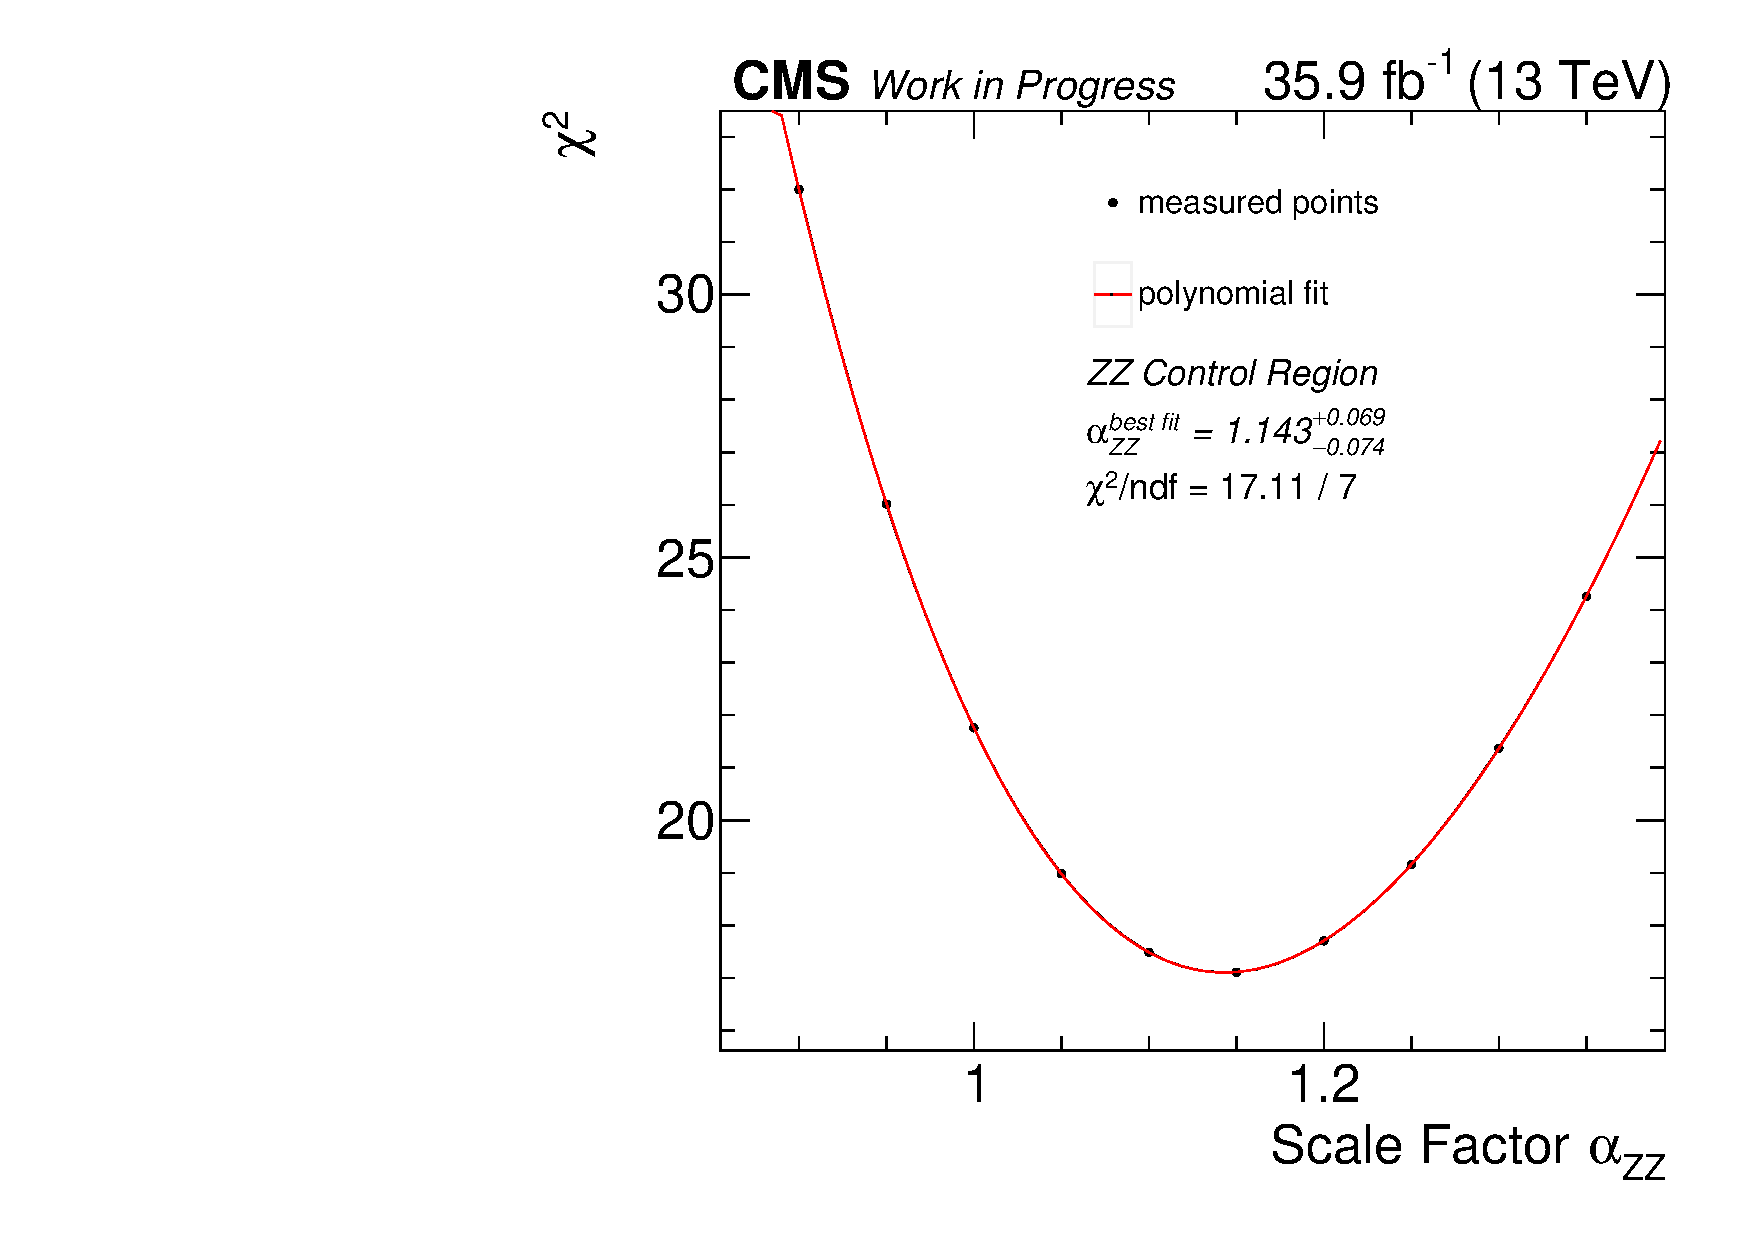
\includegraphics[width=\pairwidth]{figures/plots_CR/chi/ZZ_met}
 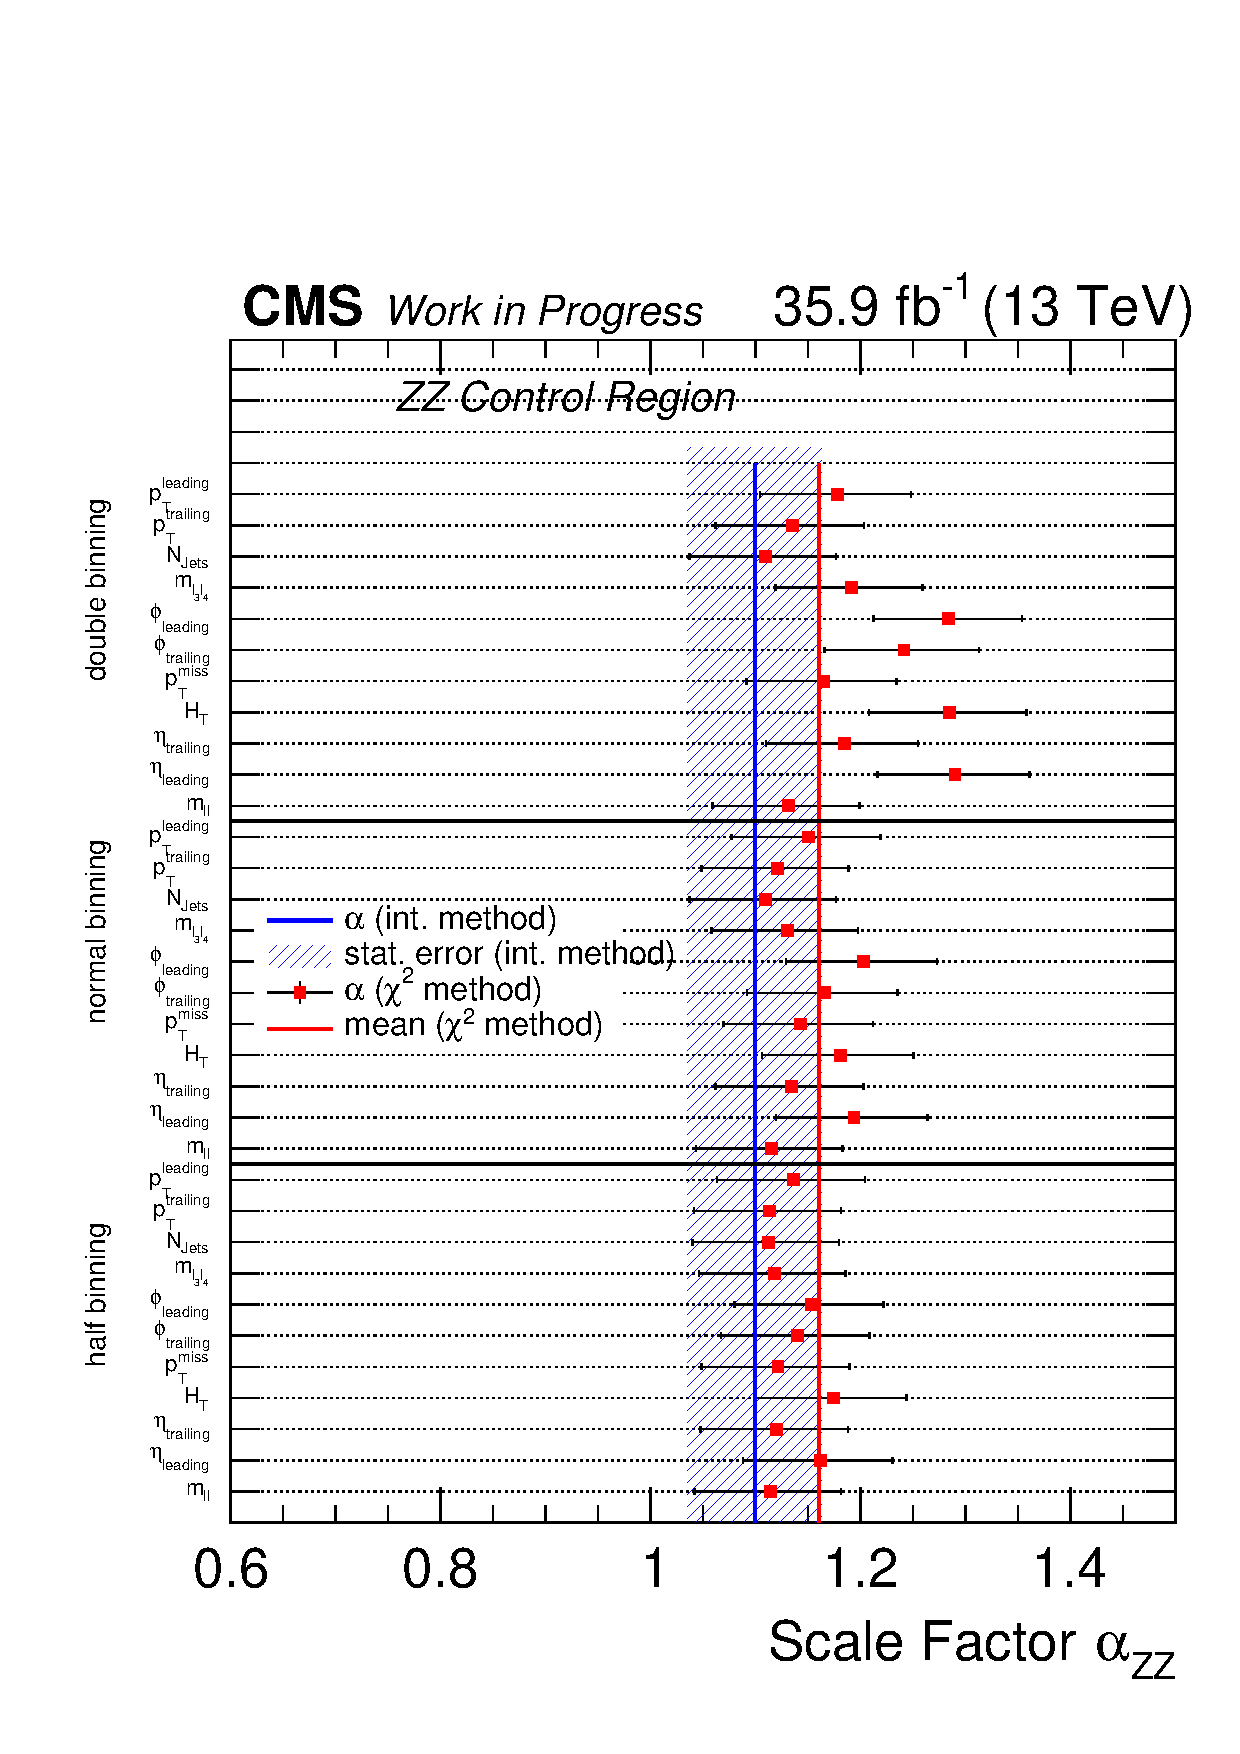
\includegraphics[width=\pairwidth]{figures/plots_CR/chi/ZZ_Compare}
 \caption{Example $\chi^2$ fit in the $\PZ\PZ$ CR in the $\ptmiss$ distribution (left) with the polynomial fit. All fit results compared with the SF obtained from the integral method in different binnings and variables (right.)}
 \label{fig:chiZZ}
\end{figure}

\subsection{Other standard model backgrounds}
Additional minor backgrounds, such as triboson processes as $\PW\PZ\PGg$, $\PW\PW\PGg$, diboson $\PW\PW$ and $\PW\PGg$ production, the production of $\PW$ bosons in association with jets, and single top processes as listed in \refTab{tab:MCsamples}, are taken from plane simulation after reweighting them as described in \refSec{sec:Simulation} to the measured luminosity and NLO and NNLO cross sections.

\FloatBarrier
\subsection{Validation of the background estimation}\label{sec:Validation}
After all main backgrounds are tuned in various corresponding CRs and SFs are determined, and the remainder is taken from pure simulation, the background prediction is validated in the VR defined in \refSec{sec:VR}. In phasescpace it is very close to the SR where the background prediction shall work sufficiently well, and therefore the VR is ideal to study the obtained background prediction.\\
Resulting comparisons between prediction and observed data in different distributions are shown in \refFig{fig:VR1} for the most important variables, such as $\ptmiss$ and $\mtTwo$, together with $\pt$ distributions of the leading and trailing lepton. Comparisons for the photon $\pt$ and the invariant dilepton mass $m_{\ell\ell}$ distributions are shown in \refFig{fig:VR2}.\\
Overall, the agreement is very good in all distributions, although being limited by the lower statistics in some kinematic regions. The same Kolmogorov-Smirnov tests as for the different CRs are performed to gain more trust in the background prediction. As can be read from the resulting KS-values, each quoted on the corresponding plot, the shape agreement considering statistical uncertainties and systematic uncertainties originating from the statistical ones from the integral method, is very good. With $97$ data events measured and $93.6$ predicted, the total agreement is very good.\\
Therefore, the background prediction is assumed to work fine in the SR due to the similar kinematics in the VR based on the design as a kinematic sideband in $\ptmiss$ and $\mtTwo$.
\begin{figure}[tbp]
 \centering
 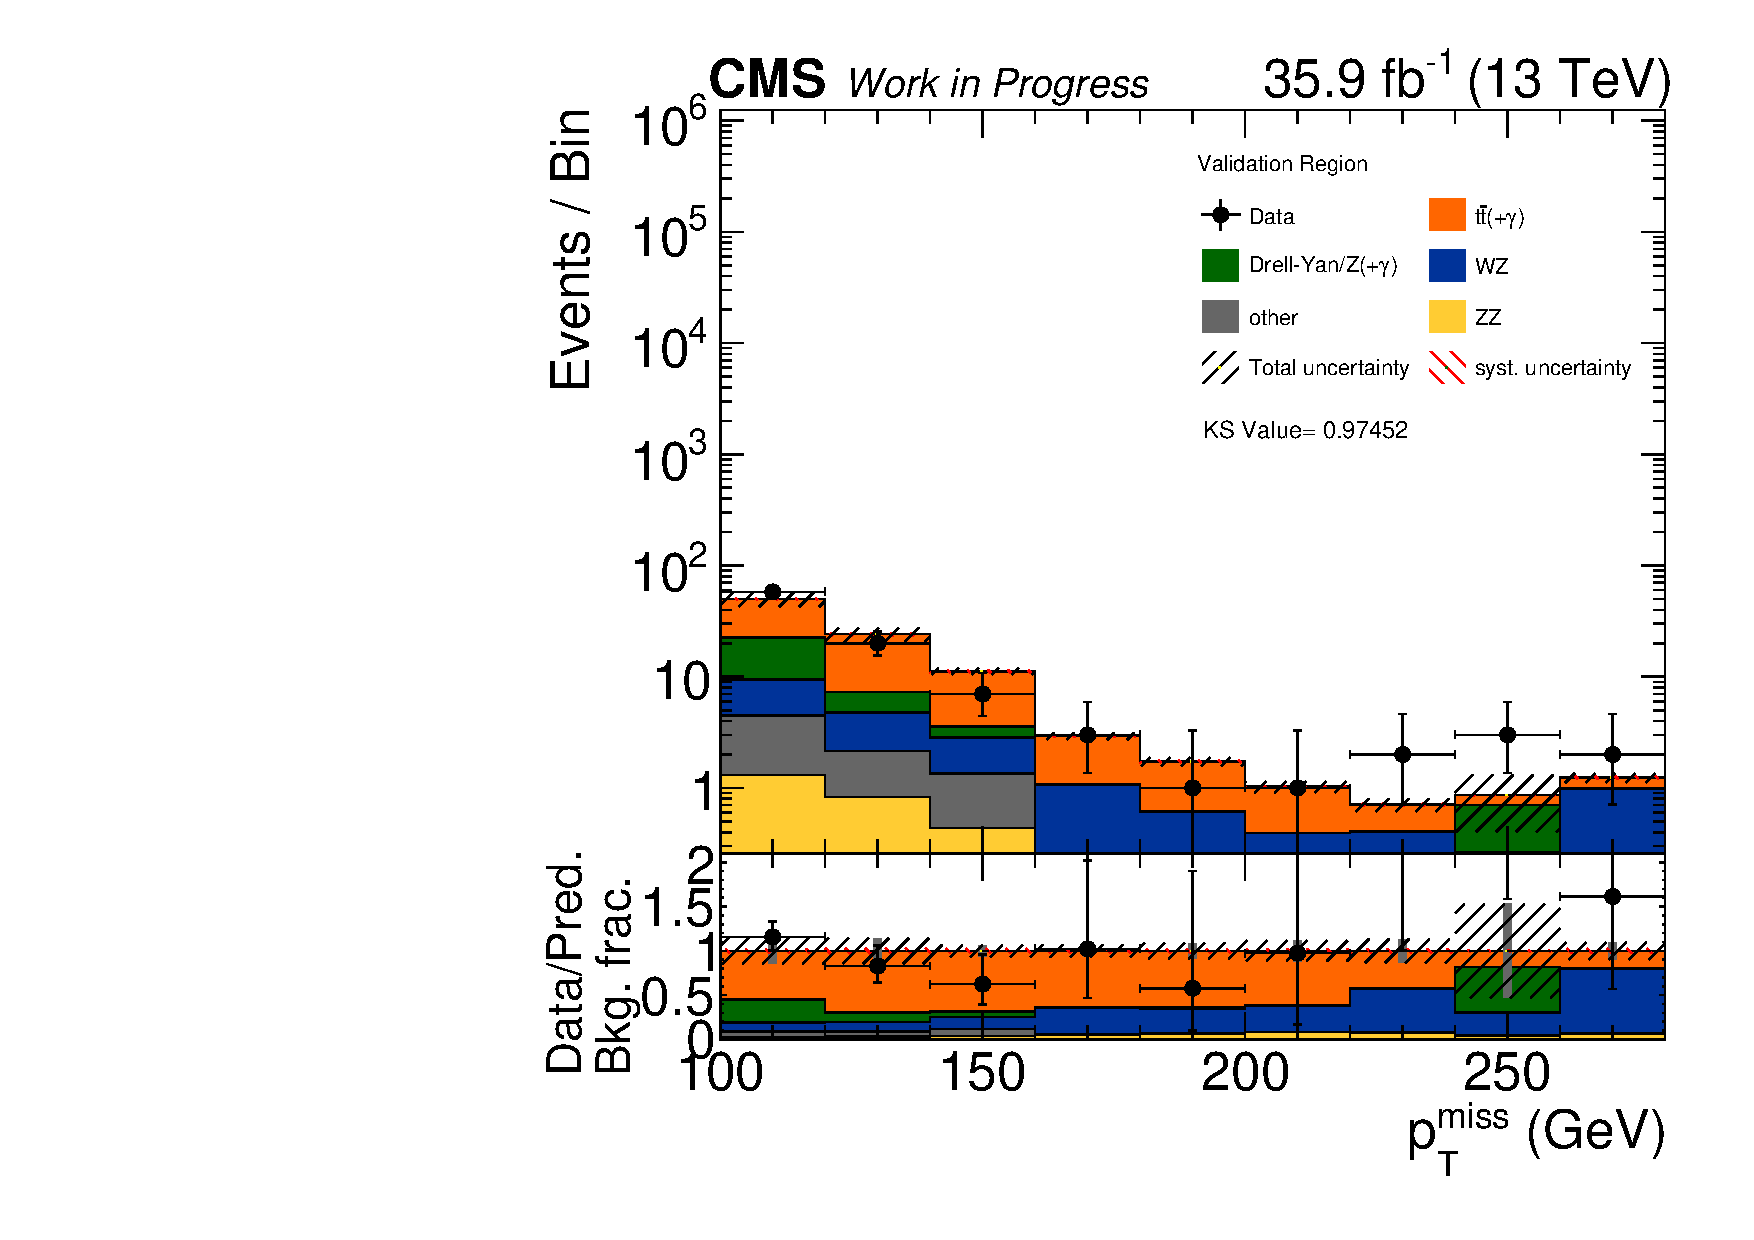
\includegraphics[width=\pairwidth]{figures/plots_VR/VR_LL_met_log}
 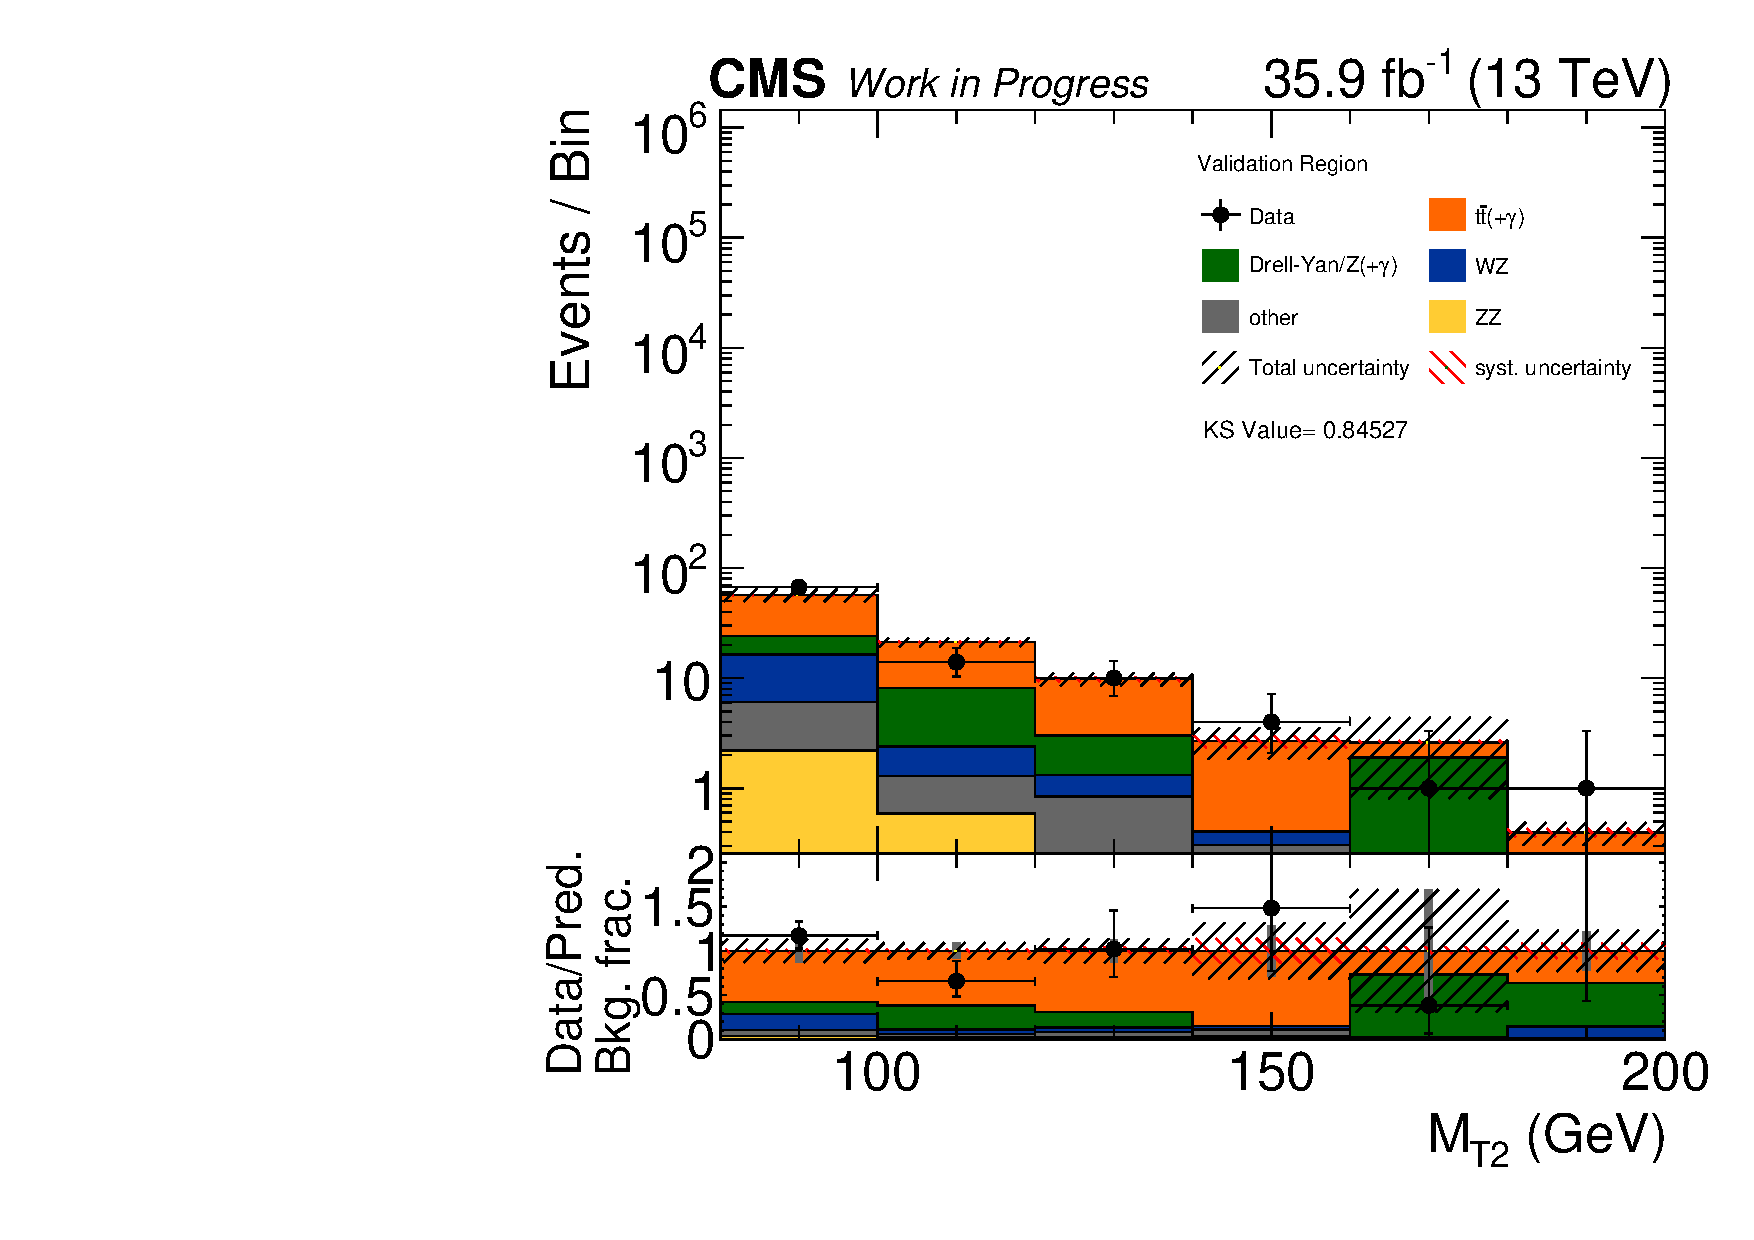
\includegraphics[width=\pairwidth]{figures/plots_VR/VR_LL_mt2_log}\\
 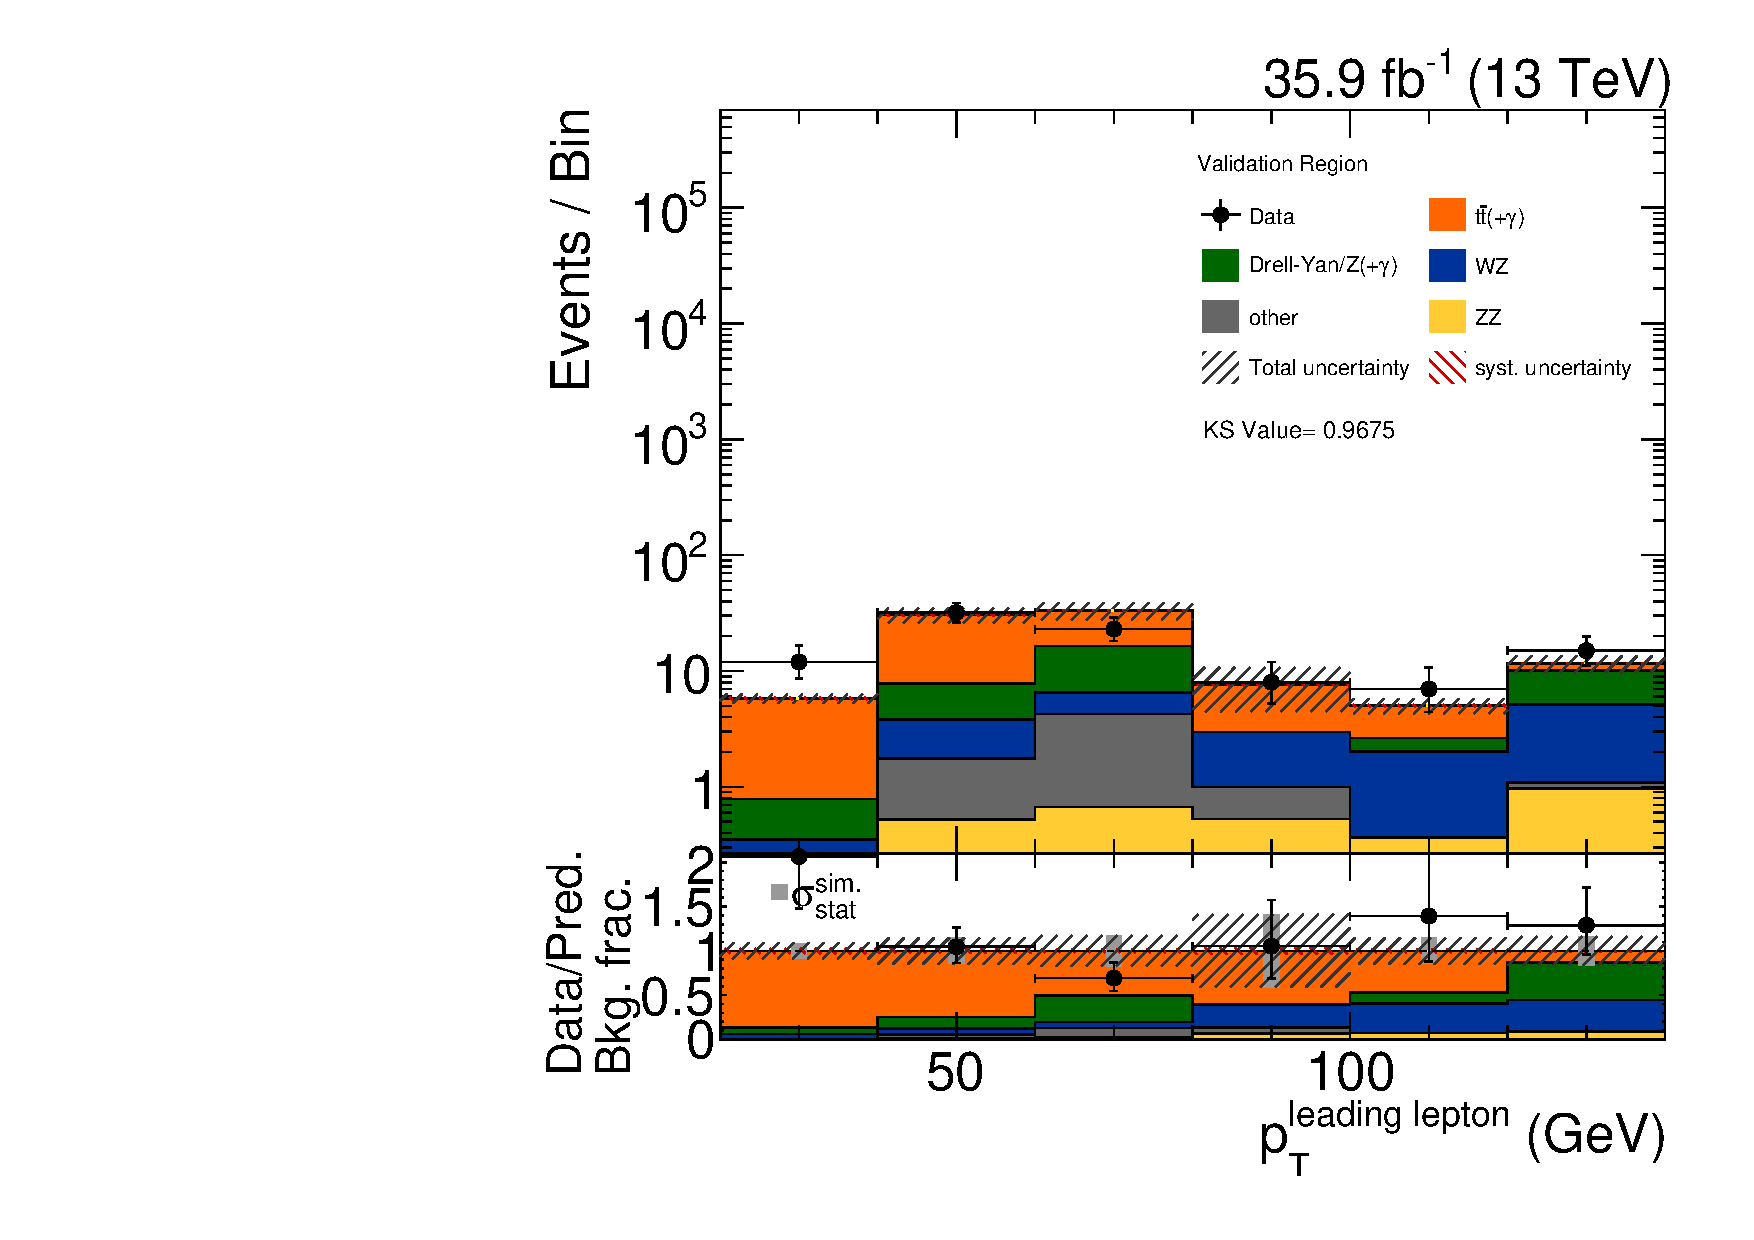
\includegraphics[width=\pairwidth]{figures/plots_VR/VR_LL_pt1_log}
 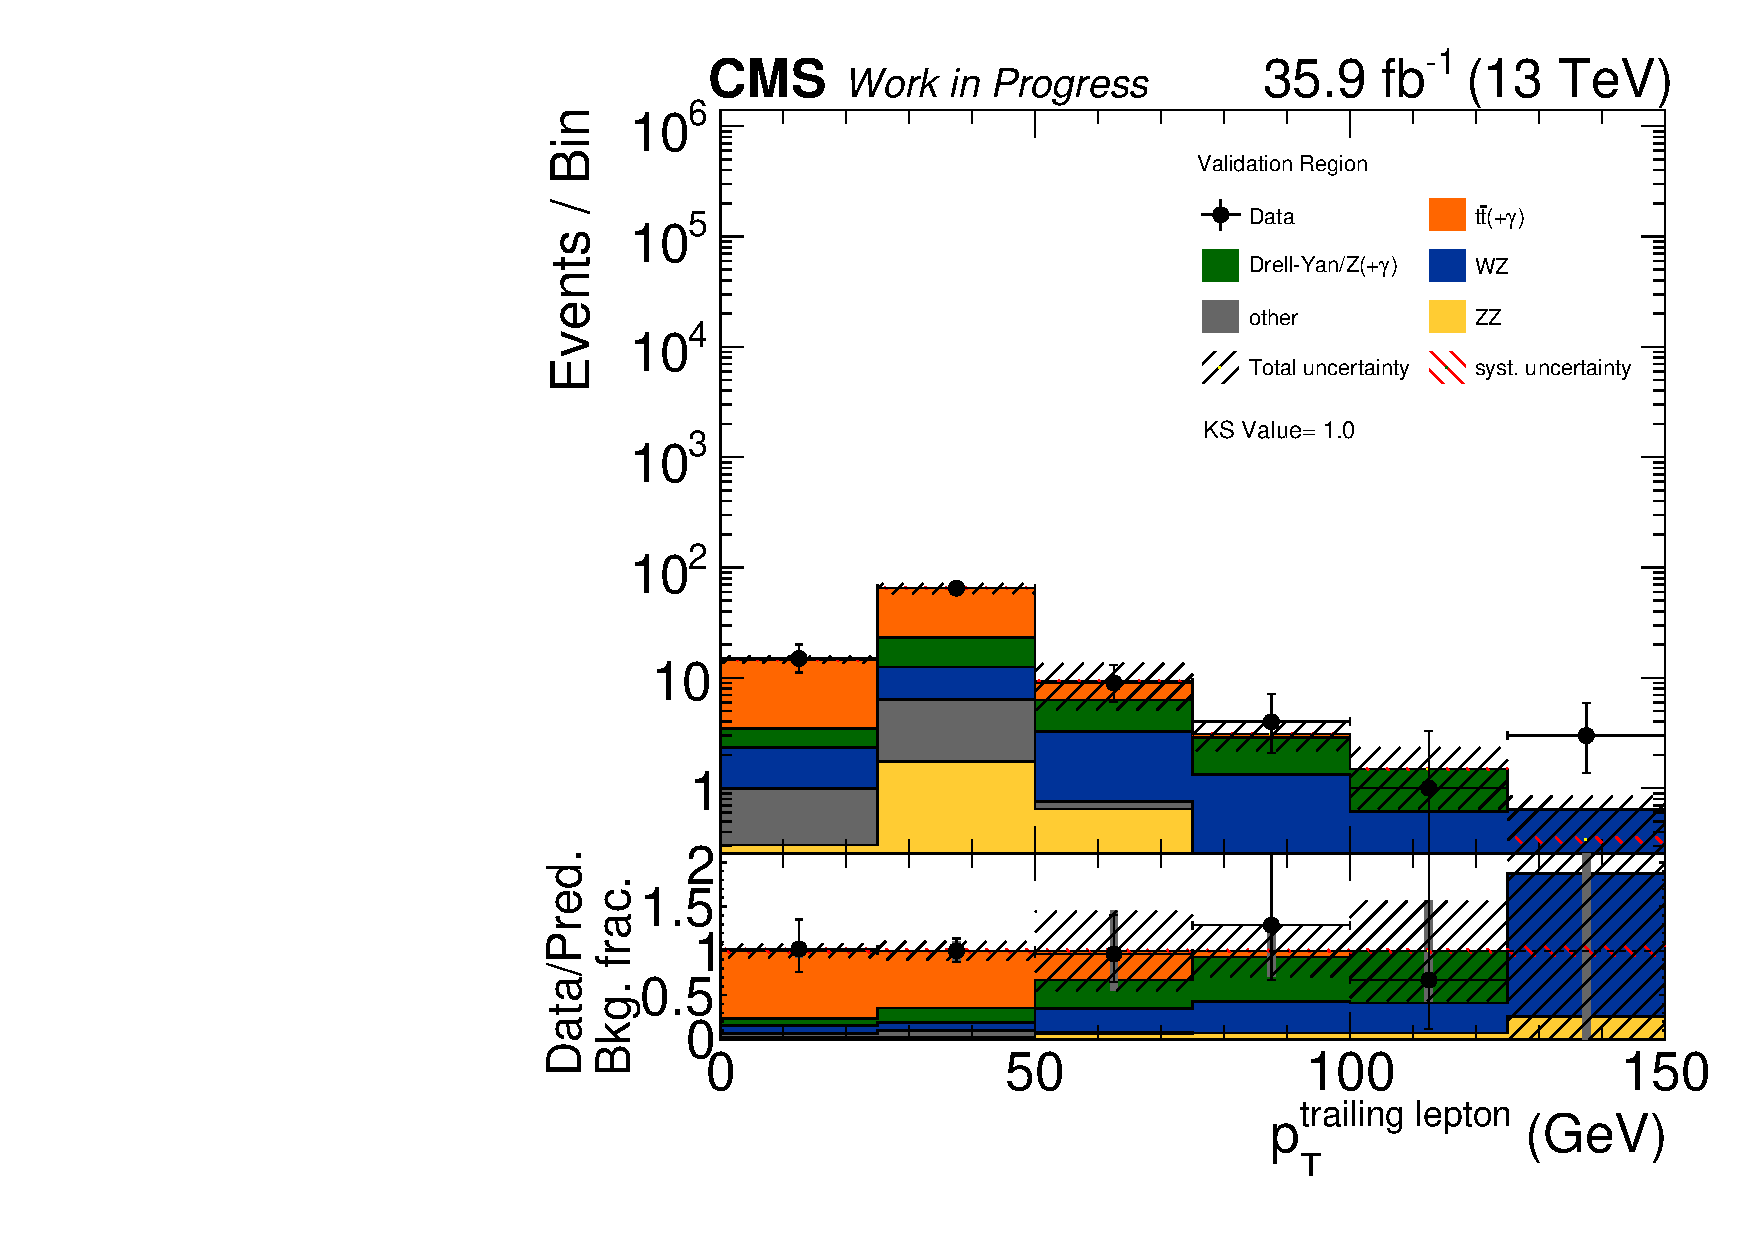
\includegraphics[width=\pairwidth]{figures/plots_VR/VR_LL_pt2_log}
 \caption{Comparisons between data and rescaled simulation in theVR in the $\ptmiss$, $\mtTwo$, and lepton $\pt$ distributions. Below each plot, a ratio between data and prediction is shown. The uncertainty bands correspond to the systematic (re) and total uncertainty (gray). In addition, in the ratio plot the relative compostion of the backgrounds is visualized. KS-values for the performed Kolmogorov-Smirvov test are also quoted.}
 \label{fig:VR1}
\end{figure}


\begin{figure}[tbp]
 \centering
 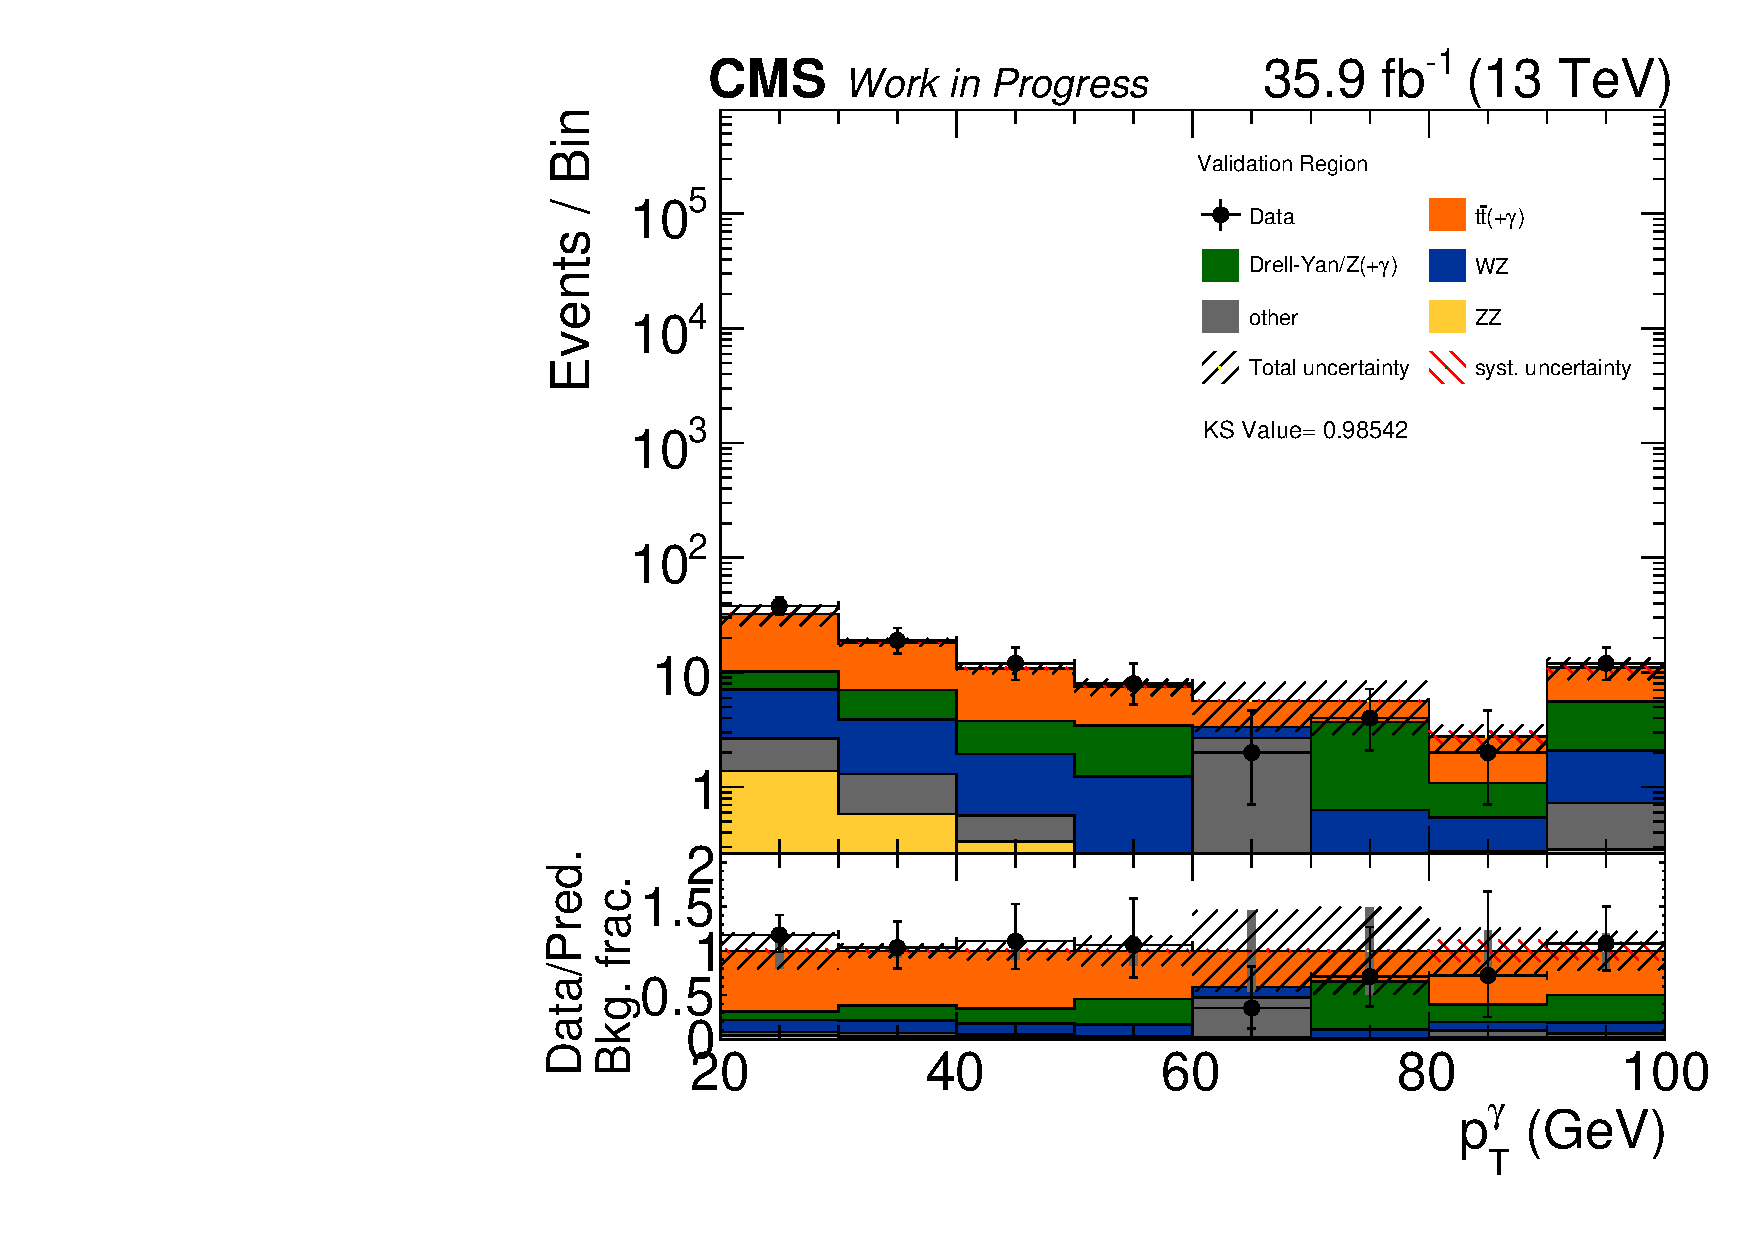
\includegraphics[width=\pairwidth]{figures/plots_VR/VR_LL_pt_g1_log}
 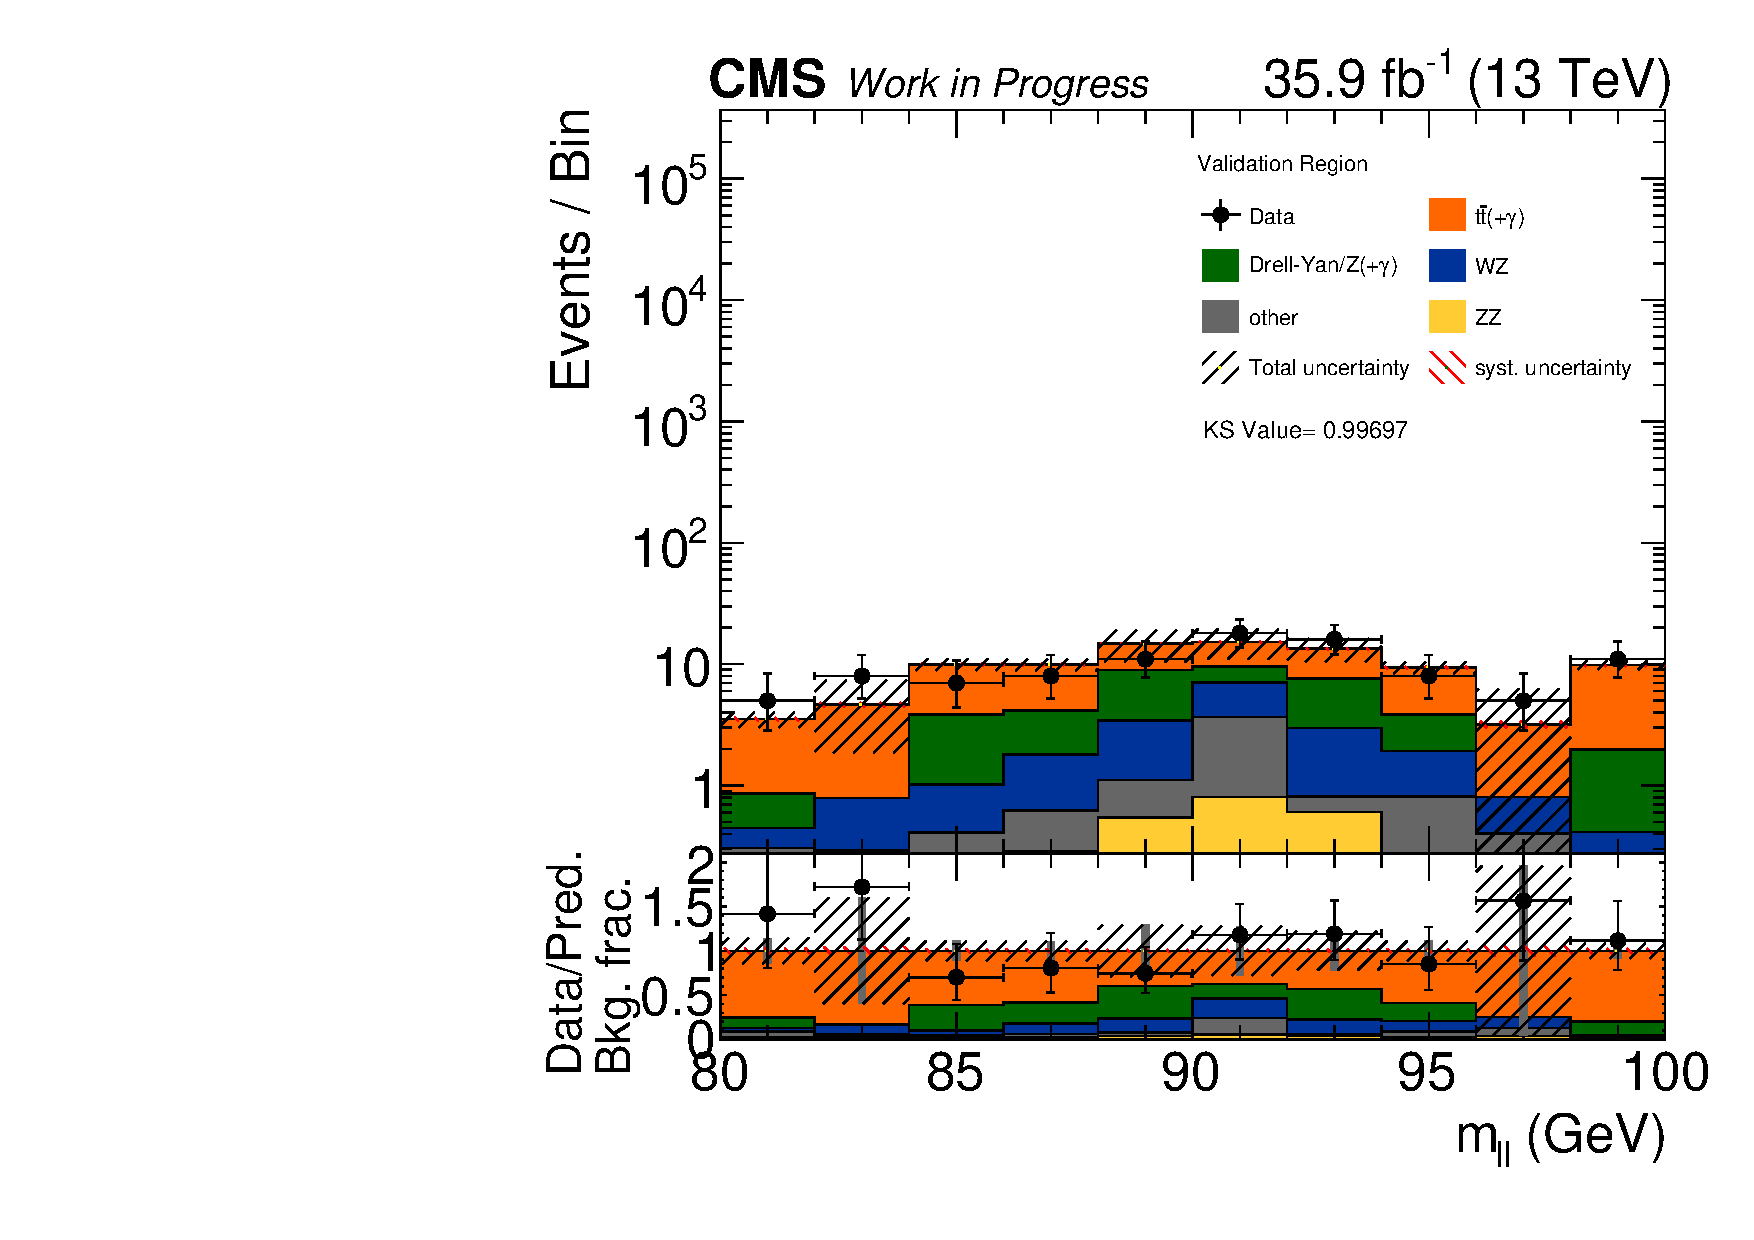
\includegraphics[width=\pairwidth]{figures/plots_VR/VR_LL_m_ll_log}
 \caption{Comparisons between data and rescaled simulation in the VR in the photon $\pt$ and invariant dilepton mass distribution. Below each plot, a ratio between data and prediction is shown. The uncertainty bands correspond to the systematic (red) and total uncertainty (gray). In addition, in the ratio plot the relative compostion of the backgrounds is visualized. KS-values for the performed Kolmogorov-Smirvov test are also quoted.}
 \label{fig:VR2}
\end{figure}


\subsection{Signal contamination}\label{sec:signalCont}
If case of measurable SUSY signals, it would of course not only produce events being observable in the SR, but also some of them may appear in the CRs that are used to determine a proper background prediction. To account for this effect, the so-called signal contamination of the background CRs is not considered in the background estimation itself, but is rather translated into a reduction of the predicted signal yield in the SR. Hence, at first the signal contamination needs to be measured for each signal point of all samples individually in all CRs.\\
Therefore, the fraction of expected signal events relative to the total amount of background events in each CR is measured. Examples for the contamination of the \texttt{TChiZG} SMS in the DY/$\PZ(\PGg)$ CR and the GMSB model in the $\PW\PZ$ CR are shown in \refFig{fig:signalCont}, because they are the largest ones observed. As can be seen, the contributions of signal events are mainly negligible, although the signal contamination reaches $\approx 3\%$ for very low bino and wino masses in the GMSB model.\\
To account for those effects, these relative fractions are used to lower the signal expectation in each SR bin individually. This can be accomplished in a simple way, since the background prediction method is based on simulation which is rescaled with constant SFs. If $\rho$ is the fraction of signal events in the CR, in each SR bin the absolute signal event yield reduced with the following formula
\begin{equation}
 \#signal_{after} = \#signal_{before} - \rho\cdot\#background,
\end{equation}
where $\#signal_{before}$ and $\#signal_{after}$ are the total number of signal events per bin before and after the correction, and $\#background$ is the number of predicted background events in this bin.

\begin{figure}
 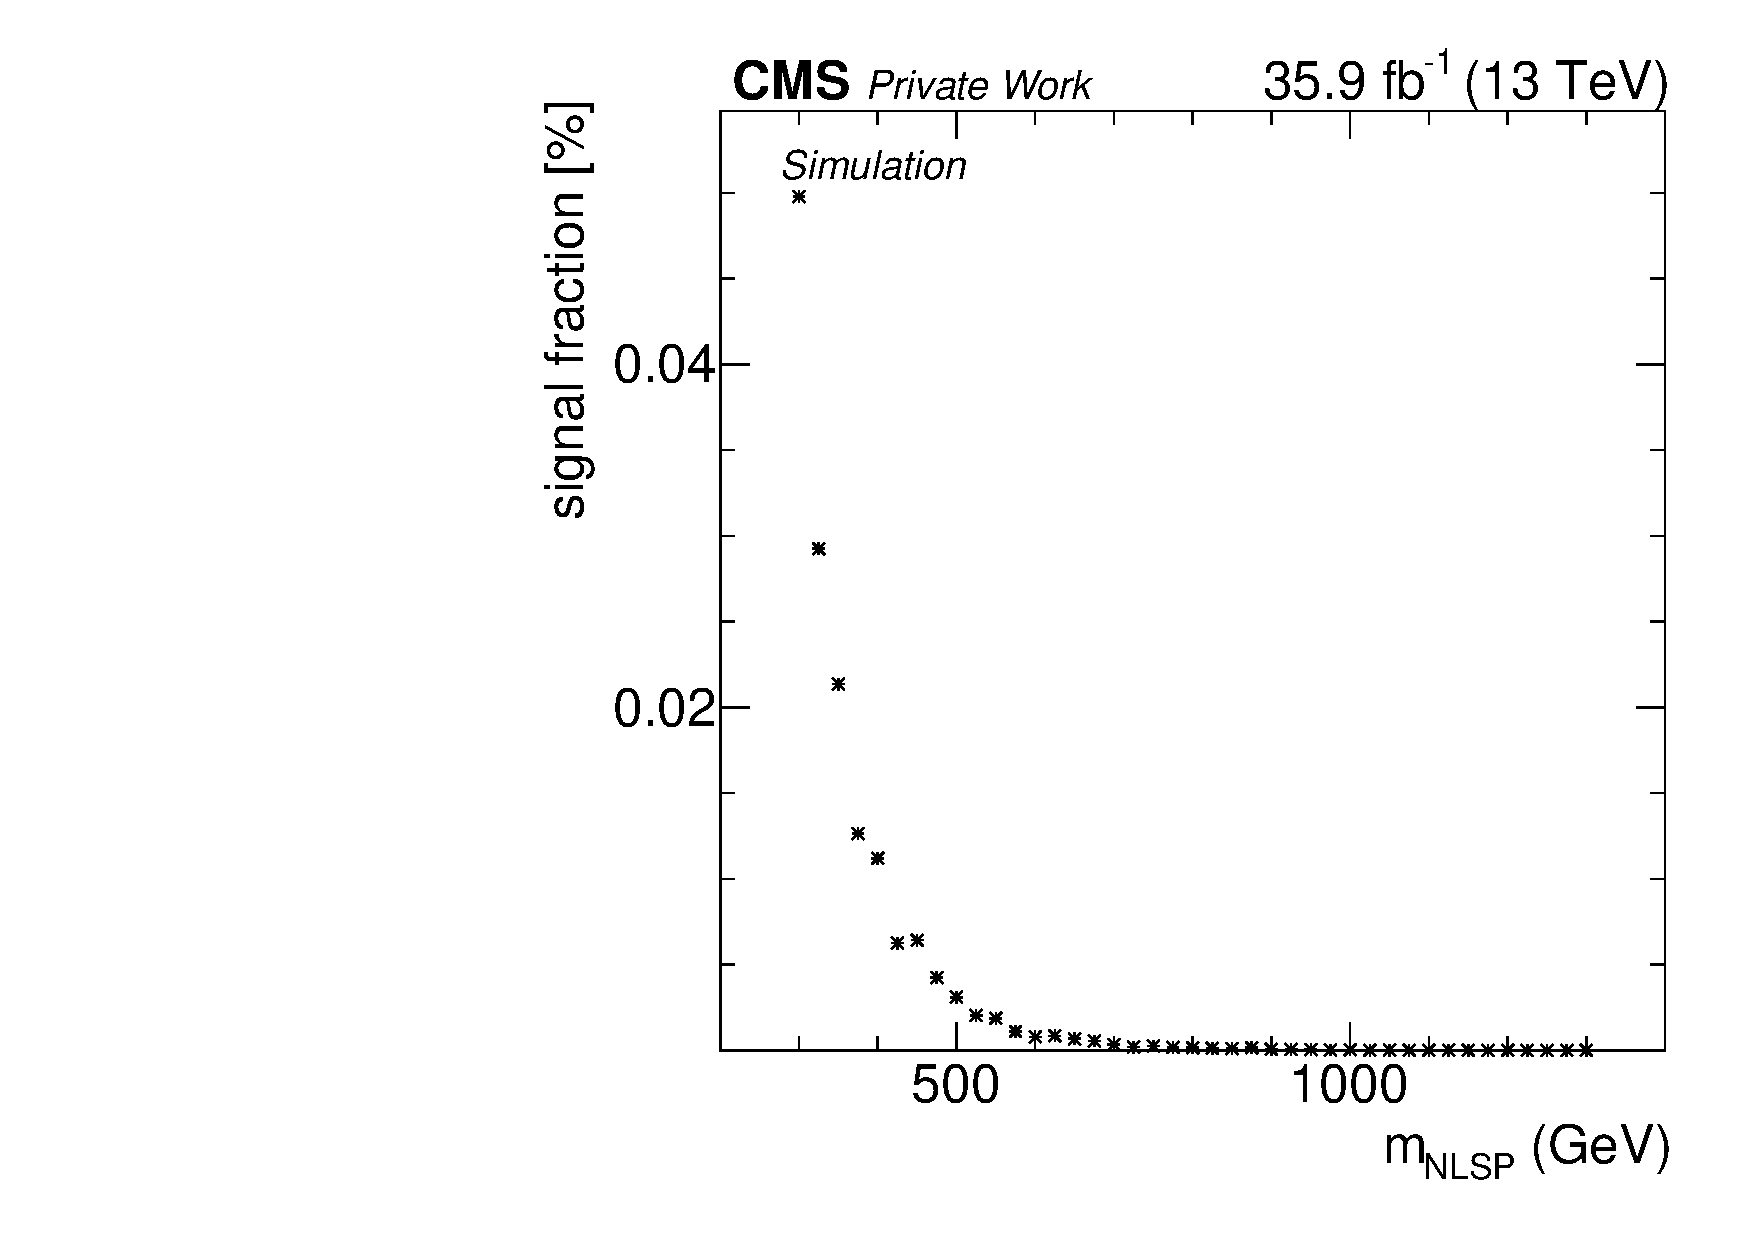
\includegraphics[width=\pairwidth]{figures/contamination/tching_DY}
 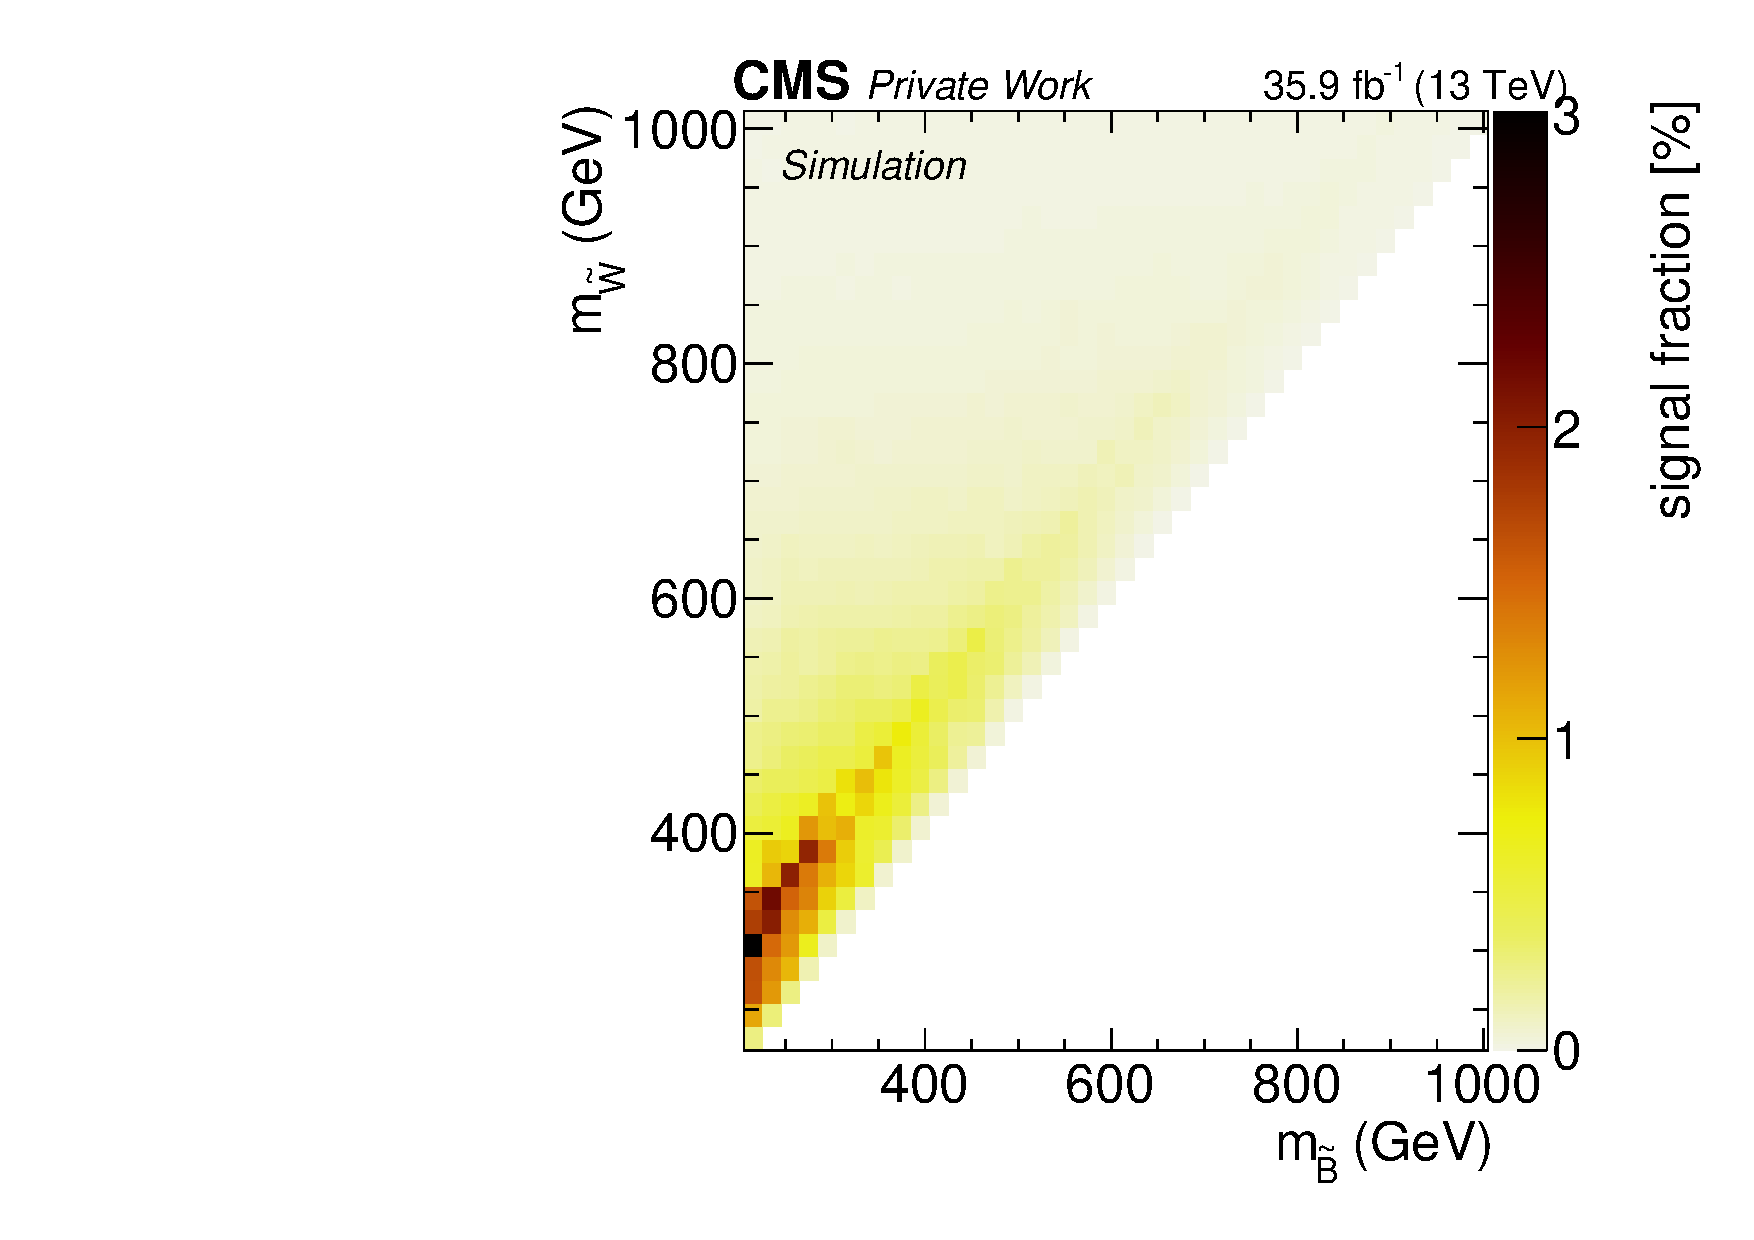
\includegraphics[width=\pairwidth]{figures/contamination/gmsb_WZ}
 \caption{Signal fraction for different signal points of the \texttt{TChiZG} in the DY/$\PZ(\PGg)$ CR (left) and the GMSB model in the $\PW\PZ$ CR (right).}
 \label{fig:signalCont}
\end{figure}
In total, the influence of signal contamination to the final result is rather negligible, because for most of the signal points the contributions to all CRs are very low. In cases where they exceed the level of some percent, their influence will not matter in the final interpretation, since for those low SUSY mass signal points, the expectation for the signal yield in the SR is sufficiently high enough.


\section{Study of systematic uncertainties}\label{sec:Syst}
In addition to the statistical uncertainties coming from the background prediction method itself, various systematic effects and their impact on the final prediction need to be evaluated.

\subsection{Background uncertainties}
Sources of systematic uncertainties arise from the measured pileup distribution,  which is needed to rescale the simulated samples as explained in \refSec{sec:Simulation}, the measurement of the total integrated luminosity, the measurement of the jet energy scale (JES) and the jet energy resolution (JER), that are important for the $\ptmiss$ description, the measured trigger efficiencies as discussed in \refSec{sec:triggEff}, corrections for a different photon and lepton reconstruction in simulation and data, the PDF used in the MC simulation process, and the factorization scale and renormalization scale.\\
These measurements and underlying effects all provide systematic uncertainties on the final background prediction. Cross section, trigger, and luminosity uncertainties cancel for the four main background contributions due to the applied method, but are relevant for the other minor contributions as a relative uncertainty. They are assumed to be $50\%$ to account for the biggest differences between the measurement and theoretical prediction, and consider the circumstance, that only a special phase space is used in the analysis.\\
The uncertainty on the luminosity measurement with $2.5\%$~\cite{LumiUncert} and the uncertainty on the trigger efficiency, that is estimated to be $3\%$ (see \refSec{sec:triggEff}), propagate directly as relative uncertainties to the final prediction.\\
All other uncertainties are uncertainties in the shape, and need to be determined another way. In order to estimate the impact of the JEC and JER, the pileup reweighting, and the lepton and photon identification and reconstruction corrections, the whole background prediction is performed again with the underlying quantities shifted one standard deviation up and down. Hence, two additional predictions for each SR bin are obtained, and half of the difference between those, relative to the nominal prediction, is taken as the systematic uncertainty.\\
To estimate the effect on the choice of the renormalization scale $\mu_R$ and factorization scale $\mu_F$, these two are varied in combinations of the factors $0.5$, $1$, and $2$, and nine new background predictions are obtained. The half of the difference between the two outliers, relative to the nominal prediction, is treated as the systematic uncertainty.\\
To determine the systematic uncertainty arising from the used PDFs, one hundred different PDF variations are studied, and for each the background prediction method is performed again, thus one hundred different predictions for the SR are obtained. From this distribution of predicted yields, the standard deviation and the mean can be calculated. The standard deviation normalized to the mean is considered as the systematic uncertainty.\\
The uncertainty arising from the choice of order regarding the four SFs determined in the CRs, is estimated by testing all $4!=24$ possibilities, and calculating the largest deviation from the nominal SFs. This envelope is considered as a systematic uncertainty on the SFs on top of the statisical uncertainty. Both uncertainties are added quadratically, such that one final uncertainty for each SF is obtained.
\refTab{tab:systuncBKG} lists ranges for all final systematic uncertainties for all backgrounds individually.
\begin{table}[tbp]
 \centering
 \caption{Systematic uncertainty ranges for all background predictions in the signal region.}
 \small
 \label{tab:systuncBKG}
 \begin{tabular}[width=\textwidth]{llllll}
                               & $tt(\PGg)$  & DY/Z$(\PGg)$  & $\PW\PZ$    & $\PZ\PZ$    & Other       \\\hline
  PDF                          & $0.8-1.5\%$ & $2.6-3.3\%$   & $0.5-0.7\%$ & $2.2-2.4\%$ & $1.1-1.2\%$ \\
  Renorm. and fact. scale      & $3.3-7.1\%$ & $18.2-22.5\%$ & $4-6\%$     & $3.7-4.1\%$ & $2.1-9.3\%$ \\
  JES                          & $4.6-6.5\%$ & $4.4-5\%$     & $2.8-4.8\%$ & $1-1.9\%$   & $0-50.7\%$  \\
  JER                          & $1.6-3.1\%$ & $0.7-16.1\%$  & $1-1.8\%$   & $0.2-1.4\%$ & $0-50.7\%$  \\
  Lepton ID and reconstruction & $2.8-2.9\%$ & $2.2-3.4\%$   & $3.3\%$     & $1.8\%$     & $4.2\%$     \\
  Photon ID and reconstruction & $0.7-0.8\%$ & $1.4-1.5\%$   & $1-1.1\%$   & $0.9\%$     & $0.7-1.9\%$ \\
  Luminosity                   & -           & -             & -           & -           & $2.5\%$     \\
  Pileup                       & $1.2-2\%$   & $1-5\%$       & $0.2-2.5\%$ & $1.5-1.7\%$ & $0.1-10\%$  \\
  Trigger efficiency           & -           & -             & -           & -           & $3\%$       \\
  Scale factor $\alpha_{i}$    & $4.1\%$     & $0.9\%$       & $3.9\%$     & $5.7\%$     & -           \\
  Cross section                & -           & -             & -           & -           & $50\%$      \\
  \hline
 \end{tabular}
\end{table}
Besides uncertainties for some backgrounds, such as DY/$\PZ(\PGg)$ and the other composed backgrounds, exceed the level of $10\%$, where statistical fluctuations based on changes of different quantities play an important role, all other systematic uncertainties are of the order of some percent. This reflects the stability and robustness, that was observed in the scale factor determination itself.


\subsection{Signal uncertainties}
Whereas all derivations of systematic uncertainties on the final event yields are covered, further signal uncertainties need to be studied in order to interpret the results statistically in each SUSY model.
Most of the signal uncertainty determination methods behave the same as explained above for the backgrounds, but some additional effects need to be considered, and some calculations change, since the detector response in the signal MC simulation was performed using \FASTSIM.\\
For the determination of the pileup uncertainty, a different method was applied. The pileup distribution is split into a low PU ($<20$) and a high PU ($>20$) region, and the difference in the total signal acceptance was determined. Half of this difference is treated as the systematic uncertainty.\\
Because the modeling of the $\ptmiss$ distribution is very complicated, and in the \FASTSIM package only a simplified detector response is parameterized, the difference between generated $\ptmiss$ and reconstructed $\ptmiss$ is investigated. Thus, the whole analysis is reperformed for the signal, where the reconstructed $\ptmiss$ is replaced with the generated one for each event, and the difference in the acceptance is examined. Half of the deviation is taken as the systematic uncertainty.\\
For the signal simulation no PDF uncertainties are available. In addition, the initial state radiation dependent reweightings mentioned in \refSec{sec:Simulation} introduce systematic effects on the signal yield expectation. Therefore the same method as mentioned above for the identification and reconstruction uncertainties on the background prediction is performed.\\
Ranges for all signal uncertainties including the statistical one are given in \refTab{tab:systuncSignal} altogether for all signal models considered in the analysis.
\begin{table}[tbp]
 \centering
 \caption{Ranges for all the systematic uncertainties for all signal models.}
 \normalsize
 \label{tab:systuncSignal}
 \begin{tabular}[width=\textwidth]{ll}
  Uncertainty         & Range $[\%]$ \\\hline
  Statistical         & $3.2-85$     \\
  Luminosity          & $2.6$        \\
  PileUp              & $<0.1-143$   \\
  JES                 & $<0.1-62$    \\
  JER                 & $<0.1-63$    \\
  Trigger Efficiency  & $3$          \\
  Lepton Scale Factor & $<0.1-5.6$   \\
  Photon Scale Factor & $1.4-1.5$    \\
  MET/GEN MET         & $<0.1-293$   \\
  ISR Reweighting     & $<0.1-10.5$  \\
  Scale               & $0.1-10.9$   \\
  \hline
 \end{tabular}
\end{table}
Large ranges are observable due to the limited statistics that is available for each signal point. Mainly all other systematic effects are correlated with the statistical uncertainty. This is due to time and resource saving reasons, since a huge amount of different signal points is being generated. In addition, the already low amount of generated signal events becomes much lower, as only leptonic decay branches of the Z boson are considered and this branching fraction is very low. Nevertheless, in most of the relevant signal points the uncertainties do not exceed the level of a few percent.
